%------------------------------------------------------------------------
%- Reference for the EALib                                              -
%------------------------------------------------------------------------
%- History of modification                                              -
%-                                                                      -
%-  ver.1.01 : 2000/05/29 Ruediger Alberts (Institut fuer               -
%-                        Neuroinformatik, Bochum)                      -
%-               original                                               -
%-  ver.1.02 : 2001/01/04 Tatsuya Okabe (HONDA R&D EUROPE DEUTSCHLAND)  -
%-               separate files , add index                             -
%-  ver.1.03 : 2001/01/30 Tatsuya Okabe (HONDA R&D EUROPE DEUTSCHLAND)  -
%-               include some classes about random generator            -
%-  ver.1.04 : 2001/02/05 Tatsuya Okabe (HONDA R&D EUROPE DEUTSCHLAND)  -
%-               include some important classes                         -
%-  ver.1.10 : 2001/02/14 Tatsuya Okabe (HONDA R&D EUROPE DEUTSCHLAND)  -
%-               release version                                        -
%-  ver.1.11 : 2001/06/08 Tatsuya Okabe (HONDA R&D EUROPE DEUTSCHLAND)  -
%-               correct some mistakes                                  -
%-  ver.1.12 : 2002/05/22 Ruediger Alberts (ZN AG, Bochum)              -
%-               splitted parts for EALib, Array and Rng                -
%-                                                                      -
%-  ver.1.13 :                                                          -
%-                                                                      -
%-  ver.1.14 :                                                          -
%-                                                                      -
%-  ver.1.15 :                                                          -
%-                                                                      -
%------------------------------------------------------------------------

\documentclass{report}
\usepackage{a4}
\usepackage{graphicx}
\usepackage{makeidx}
\makeindex
% =======================================================================
% Dateiname:        Vorlage.tex
% Autor:            Ruediger Alberts
% EMail:            Ruediger.Alberts@neuroinformatik.ruhr-uni-bochum.de
% Erstellt am:      1999-09-07
% Letzte Aenderung: 1999-09-09
%
% Datei wird mit Befehl ``\input{Vorlage}'' in LaTex-Dokumente 
% (Latex2Epsilon) eingebunden und stellt Befehle zur einfachen Doku- 
% mentation von C-Funktionen/C++-Methoden bereit.
% =======================================================================

\usepackage{ifthen}

    % Definition von Konstanten:
    \newcommand{\ParamDelim}            % Trennungstext zwischen
        { \ - }                         % Parametername und -beschreibung.
    \newcommand{\NormMethodEnd}         % Endtext von Methode bei 
        {\ \ );}                        % veraenderbarer Aufrufinstanz.
    \newcommand{\ConstMethodEnd}        % Endtext von Methode bei
        {\ \ ) const;}                  % nicht veraenderbarer Aufrufinstanz.
    \newcommand{\MaxLabelTxt}           % Komponentenbeschreibungstext
        {{\bf Return Value: }}          % mit maximaler Breite.
    \newcommand{\MethodBegin}           % Beginntext einer Methode.
        {(\ }
    \newcommand{\InBetween}             % Text zwischen Rueckgabewert und
        {\ \ }                          % Methodenname.

    % Definition eigener Variablen:


    \newboolean{ConstInstance}          % Gibt an, ob die Instanz, die
                                        % die Methode aufruft veraendert
                                        % werden darf oder nicht. Im
                                        % 2. Fall endet die Methode mit
                                        % ``) const;'', im 1. Fall 
                                        % mit ``);''.
    \newcounter{SavedParams}            % Anzahl der gespeicherten
                                        % Parameter.
    \setcounter{SavedParams}{0}
    \newcommand{\ParamOne}{}            % Definition der 10 
    \newcommand{\ParamTypeOne}{}        % abspeicherbaren Parameter,
    \newcommand{\ParamDescrOne}{}       % ihrer Typen und Beschreibungen.
    \newcommand{\ParamTwo}{}            
    \newcommand{\ParamTypeTwo}{}
    \newcommand{\ParamDescrTwo}{}
    \newcommand{\ParamThree}{}
    \newcommand{\ParamTypeThree}{}
    \newcommand{\ParamDescrThree}{}
    \newcommand{\ParamFour}{}
    \newcommand{\ParamTypeFour}{}
    \newcommand{\ParamDescrFour}{}
    \newcommand{\ParamFive}{}
    \newcommand{\ParamTypeFive}{}
    \newcommand{\ParamDescrFive}{}
    \newcommand{\ParamSix}{}
    \newcommand{\ParamTypeSix}{}
    \newcommand{\ParamDescrSix}{}
    \newcommand{\ParamSeven}{}
    \newcommand{\ParamTypeSeven}{}
    \newcommand{\ParamDescrSeven}{}
    \newcommand{\ParamEight}{}
    \newcommand{\ParamTypeEight}{}
    \newcommand{\ParamDescrEight}{}
    \newcommand{\ParamNine}{}
    \newcommand{\ParamTypeNine}{}
    \newcommand{\ParamDescrNine}{}
    \newcommand{\ParamTen}{}
    \newcommand{\ParamTypeTen}{}
    \newcommand{\ParamDescrTen}{}
    \newlength{\MaxParamWidth}          % Breite des breitesten 
                                        % Methodenparameters.
    \newlength{\SpecialWidth}           % Breite des Textes 
    \settowidth{\SpecialWidth}          % {\bf Besonderheiten}.
        {\MaxLabelTxt}
    \newlength{\ParamDelimWidth}        % Breite des Textes `` \ - ``.
    \settowidth{\ParamDelimWidth}
        {\ParamDelim}
    \newlength{\ParamDescrWidth}        % Max. Breite des Parametertextes.
    \newlength{\SpecialRetTxtWidth}     % Max. Breite der Texte fuer
                                        % Besonderheiten und Rueckgabewert.
    \newlength{\MethodBeginWidth}       % Breite des Methodenanfangs, d.h.
                                        % ``Rueckgabewert Methodenname ( ``.
    \newlength{\BetweenParsWidth}       % Max. zur Verfuegung stehende
                                        % Breite zwischen den beiden Klammern
                                        % der Methode.
    
    \newlength{\MethodEndWidth}         % Breite des Textes ``  );'' bzw.
    \settowidth{\MethodEndWidth}        % `` ) const;''
        {\NormMethodEnd}
    \newlength{\ParamMaxTypeWidth}      % Breite des breitesten
                                        % Parameterwert-Typs. 
    \newlength{\NoneWidthOne}           % Breite des Textes ``Keine.''.
    \settowidth{\NoneWidthOne}{None.}
    \newlength{\NoneWidthTwo}           % Breite des Textes ``Keiner.''.
    \settowidth{\NoneWidthTwo}{None.}
    \newlength{\Temp}                   % Temporaere Hilfsvariable. 
    \newlength{\VertSpace}              % Vertikaler Abstand zwischen 
                                        % zwei Parboxen.
   
    % Trotz der automatischen Berechnung der Textbreiten treten
    % kleine Unstimmigkeiten von wenigen Punkten bei den Texten
    % zur Beschreibung der Parameter, des Rueckgabewertes und
    % der Besonderheiten auf, die mit den folgenden Variablen
    % behoben werden koennen:

    \newlength{\CorrectWidthOne}        % Korrekturbreite fuer die
                                        % Parameterbeschreibung.
    \newlength{\CorrectWidthTwo}        % Korrekturbreite fuer die
                                        % Beschreibungen von Rueckgabewert
                                        % und Besonderheiten.
    \newlength{\CorrectWidthThree}      % Korrekturbreite, da erster
                                        % Parameter einer Methode weiter
                                        % vorrueckt als die anderen.
    

% Uebersicht ueber die Parameter und ihre Bedeutung.


%
% <-- \MethodBeginWidth    -->
%------------------------------------------------------------------------
% Rueckgabewert Methodenname(   Typ_Parameter_1 Parameter_1,
%                            <->Typ_Parameter_2 Parameter_2,
%              \CorrectWideThree...
%                               Typ_Parameter_n Parameter_n   );
%                             <-------------> <--------->
%                          \ParamMaxTypeWidth \MaxParamWidth
%                             <-------------------------->
%                             \BetweenParsWidth
%                                                         <-->
%                                                         \MethodEndWidth
%------------------------------------------------------------------------
% Beschreibung der Methode...
%                             \ParamDelimWidth
%                             <->                        \CorrectWidthOne
% \VertSpace
% Parameter:       Parameter_1  - Beschreibung von Parameter 1.   <----->
%                  Parameter_2  - Beschreibung von Parameter 2.
%                  ...
%                  Parameter_n  - Beschreibung von Parameter n.
% \VertSpace                      \ParamDescrWidth
%                                 <------------------------------>
% Rueckgabewert:   Beschreibung des Rueckgabewertes bzw. der Text <-----> 
%                  Keiner.                   
%                  <----->
%                  \NoneWidthTwo               \SpecialRetTxtWidth
% \VertSpace       <--------------------------------------------->
% Besonderheiten:  Beschreibung von Besonderheiten bzw. der Text  <----->
%                  Keine.     
% <--------------> <---->
%  \SpecialWidth   \NoneWidthOne                         \CorrectWidthTwo


    % Definition eigener Befehle:


    %-----------------------------------------------------------------------
    % Gibt den Begriff ``C++'' in ansprechender Form aus.
    % Makro wurde freundlicherweise zur Verfuegung gestellt von
    % Axel W. Dietrich.
    %
    \newcommand{\cpp}{
        \mbox{\emph{\textrm{C\hspace{-1.5pt}\raisebox{1.75pt}{\scriptsize +}
        \hspace{-6pt}\raisebox{.75pt}{\scriptsize +}}}}%
    }


    %-----------------------------------------------------------------------
    % Gibt die Werte aller Parameter auf dem Bildschirm aus.
    %
    \newcommand{\showAllParams}{
        \noindent
        {\em Werte aller Parameter:}
        \begin{tabbing}
            ParamMaxTypeWidth:\ \ \=\kill
            MaxParamWidth:       \>\the\MaxParamWidth\\
            SpecialWidth:        \>\the\SpecialWidth\\
            ParamDelimWidth:     \>\the\ParamDelimWidth\\
            ParamDescrWidth:     \>\the\ParamDescrWidth\\
            SpecialRetTxtWidth:  \>\the\SpecialRetTxtWidth\\
            MethodBeginWidth:    \>\the\MethodBeginWidth\\
            BetweenParsWidth:    \>\the\BetweenParsWidth\\
            MethodEndWidth:      \>\the\MethodEndWidth\\
            ParamMaxTypeWidth:   \>\the\ParamMaxTypeWidth\\
            NoneWidthOne:        \>\the\NoneWidthOne\\
            NoneWidthTwo:        \>\the\NoneWidthTwo\\
            VertSpace:           \>\the\VertSpace\\
            CorrectWidthOne:     \>\the\CorrectWidthOne\\
            CorrectWidthTwo:     \>\the\CorrectWidthTwo\\
            CorrectWidthThree:   \>\the\CorrectWidthThree\\
            ConstInstance:       
            \ifthenelse{\boolean{ConstInstance}}
                {\>ja\\}
                {\>nein\\}
        \end{tabbing}
    }

    %-----------------------------------------------------------------------
    % Setzt einen Schalter, der angibt, dass die Instanz, die die kommende
    % Methode aufrufen kann, nicht veraendert werden darf. Dies hat fuer
    % die Dokumentation zur Folge, dass die Methode mit ``) const;'' endet.
    %
    \newcommand{\setConstInstance}{    
        \setboolean{ConstInstance}{true}
    }

    %-----------------------------------------------------------------------
    % Setzt einen Schalter, der angibt, dass die Instanz, die die kommende
    % Methode aufrufen kann, veraendert werden darf. Die Methode endet also
    % in der Dokumentation normal mit ``);''.
    %
    \newcommand{\setNormalInstance}{    
        \setboolean{ConstInstance}{false}
    }

    %-----------------------------------------------------------------------
    % Initialisiert die Breite des breitesten Methodenparametertyptextes
    % mit Null.
    %
    \newcommand{\initParamMaxTypeWidth}{
        \setlength{\ParamMaxTypeWidth}{0pt}
    }

    %-----------------------------------------------------------------------
    % Initialisiert die Breite des breitesten Parameternamens mit Null.
    %
    \newcommand{\initMaxParamWidth}{
        \setlength{\MaxParamWidth}{0pt}
    }

    %-----------------------------------------------------------------------
    % Ueberprueft, ob die Breite des uebergebenen Textes des Parametertyps
    % groesser ist als die des bisher als breitester Typtext festgelegten
    % Textes und passt den Wert evtl. an.
    % Parameter #1:  Neuer Typtext, dessen Breite zum Vergleich dient.
    %   
    \newcommand{\setNewParamMaxTypeWidth}[1]{
        \settowidth{\Temp}{#1}
        \ifthenelse{\lengthtest{\ParamMaxTypeWidth < \Temp}}
            {\setlength{\ParamMaxTypeWidth}{\Temp}}{}   
    }

    %-----------------------------------------------------------------------
    % Ueberprueft, ob die Breite des uebergebenen Parameternamens groesser
    % ist als die des bisher als am breitesten geltenden Parameternames
    % und passt den Wert evtl. an. Der Parametername steht dabei in
    % Emphasized.
    % Parameter #1:  Neuer Parametername, dessen Breite zum Vergleich dient.
    %
    \newcommand{\setNewMaxParamWidth}[1]{
        \settowidth{\Temp}{{\em #1}}
        \ifthenelse{\lengthtest{\MaxParamWidth < \Temp}}
            {\setlength{\MaxParamWidth}{\Temp}}{}
    }

    %-----------------------------------------------------------------------
    % Setzt die Breite der Beschreibungstexte fuer Rueckgabewert
    % und Besonderheiten.
    %
    \newcommand{\setSpecialRetTxtWidth}{
        \setlength{\SpecialRetTxtWidth}{\textwidth}
        \addtolength{\SpecialRetTxtWidth}{-1\SpecialWidth} 
    }

    %-----------------------------------------------------------------------
    % Setzt die Breite fuer den Beginn einer Methode, d.h. den Text
    % ``Rueckgabewert Methodenname( ``. Rueckgabewert steht dabei
    % in Emphasized, Methodenname in Bold Font.
    % Parameter #1:  Rueckgabewert der Methode.
    % Parameter #2:  Name der Methode.
    %
    \newcommand{\setMethodBeginWidth}[2]{
        \settowidth{\MethodBeginWidth}
            {{\em #1}\InBetween{\bf #2}\MethodBegin}
    }

    %-----------------------------------------------------------------------
    % Setzt die maximale Breite die an Platz zwischen der oeffnenden
    % und der schliessenden Klammer der Methode zur Verfuegung steht.
    %
    \newcommand{\setBetweenParsWidth}{
        \setlength{\BetweenParsWidth}{\textwidth}
        \addtolength{\BetweenParsWidth}{-1\MethodBeginWidth}
        \addtolength{\BetweenParsWidth}{-1\MethodEndWidth}
    }

    %-----------------------------------------------------------------------
    % Setzt die Breite fuer die Beschreibungstexte
    % der Methodenparameter.
    %
    \newcommand{\setParamDescrWidth}{
        \setlength{\ParamDescrWidth}{\textwidth}
        \addtolength{\ParamDescrWidth}{-1\SpecialWidth} 
        \addtolength{\ParamDescrWidth}{-1\MaxParamWidth}
        \addtolength{\ParamDescrWidth}{-1\ParamDelimWidth}
    }    

    %-----------------------------------------------------------------------
    % Setzt die Korrekturbreite fuer den Beschreibungstext von
    % Methodenparametern auf den uebergebenen Wert.
    % Parameter #1:  Neuer Wert fuer die Korrekturbreite.
    %
    \newcommand{\setCorrectWidthOne}[1]{
        \setlength{\CorrectWidthOne}{#1}
    }    

    %-----------------------------------------------------------------------
    % Setzt die Korrekturbreite fuer den Beschreibungstext von
    % Rueckgabewert und Besonderheiten auf den uebergebenen Wert.
    % Parameter #1:  Neuer Wert fuer die Korrekturbreite.
    %
    \newcommand{\setCorrectWidthTwo}[1]{
        \setlength{\CorrectWidthTwo}{#1}
    }    

    %-----------------------------------------------------------------------
    % Setzt die Korrekturbreite fuer den Abstand des zweiten bis n-ten
    % Parameters vom Anfang auf den uebergebenen Wert.
    % Parameter #1:  Neuer Wert fuer die Korrekturbreite.
    %
    \newcommand{\setCorrectWidthThree}[1]{
        \setlength{\CorrectWidthThree}{#1}
    }    

    %-----------------------------------------------------------------------
    % Setzt den vertikalen Abstand zwischen zwei Parboxen auf den ueber-
    % gebenen Wert.
    % Parameter #1:  Neuer Wert fuer den vertikalen Abstand.
    %
    \newcommand{\setVertSpace}[1]{
        \setlength{\VertSpace}{#1}
    }    

    %-----------------------------------------------------------------------
    % Speichert die uebergebenen Informationen ueber Methodenparameter 1
    % in internen Variablen. Achtung: Die Parameter muessen in der richtigen
    % Reihenfolge gesetzt werden!
    % Parameter #1: Der Typ des Parameters.  
    % Parameter #2: Der Name des Parameters. 
    % Parameter #3: Die Beschreibung des Parameters. 
    % 
    \newcommand{\setParamOne}[3]{
        \renewcommand{\ParamOne}{#1}
        \renewcommand{\ParamTypeOne}{#2}
        \renewcommand{\ParamDescrOne}{#3} 
        \setcounter{SavedParams}{0}
        \stepcounter{SavedParams}
    }

    %-----------------------------------------------------------------------
    % Speichert die uebergebenen Informationen ueber Methodenparameter 2
    % in internen Variablen. Achtung: Die Parameter muessen in der richtigen
    % Reihenfolge gesetzt werden!
    % Parameter #1: Der Typ des Parameters.  
    % Parameter #2: Der Name des Parameters. 
    % Parameter #3: Die Beschreibung des Parameters. 
    % 
    \newcommand{\setParamTwo}[3]{
        \renewcommand{\ParamTwo}{#1}
        \renewcommand{\ParamTypeTwo}{#2}
        \renewcommand{\ParamDescrTwo}{#3} 
        \stepcounter{SavedParams}
    }

    %-----------------------------------------------------------------------
    % Speichert die uebergebenen Informationen ueber Methodenparameter 3
    % in internen Variablen. Achtung: Die Parameter muessen in der richtigen
    % Reihenfolge gesetzt werden!
    % Parameter #1: Der Typ des Parameters.  
    % Parameter #2: Der Name des Parameters. 
    % Parameter #3: Die Beschreibung des Parameters. 
    % 
    \newcommand{\setParamThree}[3]{
        \renewcommand{\ParamThree}{#1}
        \renewcommand{\ParamTypeThree}{#2}
        \renewcommand{\ParamDescrThree}{#3} 
        \stepcounter{SavedParams}
    }

    %-----------------------------------------------------------------------
    % Speichert die uebergebenen Informationen ueber Methodenparameter 4
    % in internen Variablen. Achtung: Die Parameter muessen in der richtigen
    % Reihenfolge gesetzt werden!
    % Parameter #1: Der Typ des Parameters.  
    % Parameter #2: Der Name des Parameters. 
    % Parameter #3: Die Beschreibung des Parameters. 
    % 
    \newcommand{\setParamFour}[3]{
        \renewcommand{\ParamFour}{#1}
        \renewcommand{\ParamTypeFour}{#2}
        \renewcommand{\ParamDescrFour}{#3} 
        \stepcounter{SavedParams}
    }

    %-----------------------------------------------------------------------
    % Speichert die uebergebenen Informationen ueber Methodenparameter 5
    % in internen Variablen. Achtung: Die Parameter muessen in der richtigen
    % Reihenfolge gesetzt werden!
    % Parameter #1: Der Typ des Parameters.  
    % Parameter #2: Der Name des Parameters. 
    % Parameter #3: Die Beschreibung des Parameters. 
    % 
    \newcommand{\setParamFive}[3]{
        \renewcommand{\ParamFive}{#1}
        \renewcommand{\ParamTypeFive}{#2}
        \renewcommand{\ParamDescrFive}{#3} 
        \stepcounter{SavedParams}
    }

    %-----------------------------------------------------------------------
    % Speichert die uebergebenen Informationen ueber Methodenparameter 6
    % in internen Variablen. Achtung: Die Parameter muessen in der richtigen
    % Reihenfolge gesetzt werden!
    % Parameter #1: Der Typ des Parameters.  
    % Parameter #2: Der Name des Parameters. 
    % Parameter #3: Die Beschreibung des Parameters. 
    %     
    \newcommand{\setParamSix}[3]{
        \renewcommand{\ParamSix}{#1}
        \renewcommand{\ParamTypeSix}{#2}
        \renewcommand{\ParamDescrSix}{#3} 
        \stepcounter{SavedParams} 
    }

    %-----------------------------------------------------------------------
    % Speichert die uebergebenen Informationen ueber Methodenparameter 7
    % in internen Variablen. Achtung: Die Parameter muessen in der richtigen
    % Reihenfolge gesetzt werden!
    % Parameter #1: Der Typ des Parameters.  
    % Parameter #2: Der Name des Parameters. 
    % Parameter #3: Die Beschreibung des Parameters. 
    %    
    \newcommand{\setParamSeven}[3]{
        \renewcommand{\ParamSeven}{#1}
        \renewcommand{\ParamTypeSeven}{#2}
        \renewcommand{\ParamDescrSeven}{#3} 
        \stepcounter{SavedParams} 
    }

    %-----------------------------------------------------------------------
    % Speichert die uebergebenen Informationen ueber Methodenparameter 8
    % in internen Variablen. Achtung: Die Parameter muessen in der richtigen
    % Reihenfolge gesetzt werden!
    % Parameter #1: Der Typ des Parameters.  
    % Parameter #2: Der Name des Parameters. 
    % Parameter #3: Die Beschreibung des Parameters. 
    % 
    \newcommand{\setParamEight}[3]{
        \renewcommand{\ParamEight}{#1}
        \renewcommand{\ParamTypeEight}{#2}
        \renewcommand{\ParamDescrEight}{#3} 
        \stepcounter{SavedParams}
    }

    %-----------------------------------------------------------------------
    % Speichert die uebergebenen Informationen ueber Methodenparameter 9
    % in internen Variablen. Achtung: Die Parameter muessen in der richtigen
    % Reihenfolge gesetzt werden!
    % Parameter #1: Der Typ des Parameters.  
    % Parameter #2: Der Name des Parameters. 
    % Parameter #3: Die Beschreibung des Parameters. 
    % 
    \newcommand{\setParamNine}[3]{
        \renewcommand{\ParamNine}{#1}
        \renewcommand{\ParamTypeNine}{#2}
        \renewcommand{\ParamDescrNine}{#3}  
        \stepcounter{SavedParams}
    }

    %-----------------------------------------------------------------------
    % Speichert die uebergebenen Informationen ueber Methodenparameter 10
    % in internen Variablen. Achtung: Die Parameter muessen in der richtigen
    % Reihenfolge gesetzt werden!
    % Parameter #1: Der Typ des Parameters.  
    % Parameter #2: Der Name des Parameters. 
    % Parameter #3: Die Beschreibung des Parameters. 
    % 
    \newcommand{\setParamTen}[3]{
        \renewcommand{\ParamTen}{#1}
        \renewcommand{\ParamTypeTen}{#2}
        \renewcommand{\ParamDescrTen}{#3} 
        \stepcounter{SavedParams}
    }

    %-----------------------------------------------------------------------
    % Gibt den Text ``Rueckgabewert Methodenname(`` aus.
    % Parameter #1:  Rueckgabewert der Methode.
    % Parameter #2:  Name der Methode.
    %
    \newcommand{\printMethodBegin}[2]{
         \ifthenelse{\boolean{ConstInstance}}
             {\settowidth{\MethodEndWidth}{\ConstMethodEnd}}
             {\settowidth{\MethodEndWidth}{\NormMethodEnd}}
         \setMethodBeginWidth{#1}{#2}
         \setBetweenParsWidth
         \noindent
         \hrulefill\\
         \noindent
         \parbox[t]{\MethodBeginWidth}
             {#1\InBetween{\bf #2}\MethodBegin}
     }

    %-----------------------------------------------------------------------
    % Gibt das Ende einer Methode aus, d.h. ``\ );'' oder ``\ ) const;''.
    %
    \newcommand{\printMethodEnd}{
        \ifthenelse{\boolean{ConstInstance}}
            {\ConstMethodEnd\\}
            {\NormMethodEnd\\}
            \mbox{}\hrulefill\\
    }

    %-----------------------------------------------------------------------
    % Gibt den Typen und Namen des einzigen Parameters einer Methode
    % gefolgt von dem Text ``  );'' bzw. `` ) const;'' aus.
    % Parameter #1:  Typ des Parameters.
    % Parameter #2:  Name des Parameters.
    % 
    \newcommand{\printMethodOneParam}[2]{
        \parbox[t]{\ParamMaxTypeWidth}{#1}
        \parbox[t]{\MaxParamWidth}{{\em #2}}
        \printMethodEnd
    }

    %-----------------------------------------------------------------------
    % Gibt den Typen und den Namen des ersten Methodenparameters aus.
    % Parameter #1:  Typ des Parameters.
    % Parameter #2:  Name des Parameters.
    %
    \newcommand{\printMethodFirstParam}[2]{
        \noindent
        \parbox[t]{\ParamMaxTypeWidth}{#1}
        \parbox[t]{\MaxParamWidth}{{\em #2},}\\[\VertSpace]
    }

    %-----------------------------------------------------------------------
    % Gibt den Typen und Namen des letzten Parameters einer Methode aus.
    % Parameter #1: Typ des Parameters.
    % Parameter #2: Name des Parameters.
    %
    \newcommand{\printMethodLastParam}[2]{
        \parbox[t]{\MethodBeginWidth}{\hfill}
        \hspace{\CorrectWidthThree}
        \parbox[t]{\ParamMaxTypeWidth}{#1}
        \parbox[t]{\MaxParamWidth}{{\em #2}}
        \printMethodEnd
    }

    %-----------------------------------------------------------------------
    % Gibt den Typen und Namen eines Methodenparameters aus.
    % Parameter #1:  Typ des Parameters.
    % Parameter #2: Name des Parameters.
    % Achtung: Nicht fuer den ersten oder letzten Parameter der Methode
    % geeignet!
    %
    \newcommand{\printMethodParam}[2]{
        \parbox[t]{\MethodBeginWidth}{\hfill}
        \hspace{\CorrectWidthThree}
        \parbox[t]{\ParamMaxTypeWidth}{#1}
        \parbox[t]{\MaxParamWidth}{{\em #2},}\\[\VertSpace]
    }

    %-----------------------------------------------------------------------
    % Gibt die Beschreibung einer Methode aus.
    % Parameter #1: Beschreibung der Methode.
    %
    \newcommand{\printMethodDescr}[1]{
        \newline
        \noindent
        #1\\[\VertSpace]
    }

    %-----------------------------------------------------------------------
    % Gibt den Text ``Parameter:    `` und danach den Namen des
    % ersten Parameters der Methode, gefolgt von seiner Beschreibung
    % aus.
    % Parameter #1:  Name des Parameters. 
    % Parameter #2:  Beschreibung des Parameters.
    %
    \newcommand{\printFirstParam}[2]{
        \setlength{\Temp}{\ParamDescrWidth}
        \addtolength{\Temp}{1\CorrectWidthOne}
        \parbox[t]{\SpecialWidth}{{\bf Parameters:}}
        \parbox[t]{\MaxParamWidth}{\em #1}
        \parbox[t]{\ParamDelimWidth}{\ParamDelim}
        \parbox[t]{\Temp}{#2}\\[\VertSpace]
    }

    %-----------------------------------------------------------------------
    % Gibt einen Parameter der Methode und die dazugehoerige Beschreibung
    % aus.
    % Parameter #1:  Name des Parameters.
    % Parameter #2:  Beschreibung des Parameters.
    %
    \newcommand{\printParam}[2]{
        \setlength{\Temp}{\ParamDescrWidth}
        \addtolength{\Temp}{1\CorrectWidthOne}
        \parbox[t]{\SpecialWidth}{\hfill}
        \parbox[t]{\MaxParamWidth}{\em #1}
        \parbox[t]{\ParamDelimWidth}{\ParamDelim}
        \parbox[t]{\Temp}{#2}\\[\VertSpace]
    }

    %-----------------------------------------------------------------------
    %
    % Gibt den Text ``Rueckgabewert:  `` gefolgt von einer Beschreibung
    % des Rueckgabewertes aus.
    % Parameter #1:  Beschreibung des Rueckgabewertes.
    %
    \newcommand{\printReturn}[1]{
        \setlength{\Temp}{\SpecialRetTxtWidth}
        \addtolength{\Temp}{1\CorrectWidthTwo}
        \parbox[t]{\SpecialWidth}{{\bf Return Value:}}
        \parbox[t]{\Temp}{#1}\\[\VertSpace]
    }

    %-----------------------------------------------------------------------
    % Gibt den Text ``Besonderheiten:  `` gefolgt von einer Beschreibung
    % der Besonderheiten aus.
    % Parameter #1:  Beschreibung der Besonderheiten.
    %
    \newcommand{\printSpecial}[1]{
        \setlength{\Temp}{\SpecialRetTxtWidth}
        \addtolength{\Temp}{1\CorrectWidthTwo}
        \parbox[t]{\SpecialWidth}{\bf Caveats:}
        \parbox[t]{\Temp}{#1}\\[\VertSpace]
    }

    %-----------------------------------------------------------------------
    % Gibt den Text ``Parameter:        Keine.'' aus.
    %
    \newcommand{\printNoParams}{
        \parbox[t]{\SpecialWidth}{{\bf Parameters:}}
        \parbox[t]{\NoneWidthOne}{None.}\\[\VertSpace]
    }

    %-----------------------------------------------------------------------
    % Gibt den Text ``Rueckgabewert:  Keiner.'' aus.
    %
    \newcommand{\printNoReturn}{
        \parbox[t]{\SpecialWidth}{{\bf Return Value:}}
        \parbox[t]{\NoneWidthTwo}{None.}\\[\VertSpace]
    }

    %-----------------------------------------------------------------------
    % Gibt den Text ``Besonderheiten:  Keine.'' aus.
    %
    \newcommand{\printNoSpecial}{
        \parbox[t]{\SpecialWidth}{\bf Caveats:}
        \parbox[t]{\NoneWidthOne}{None.}\\[\VertSpace]
    }

    %-----------------------------------------------------------------------
    % Gibt den Text:
    % ``Parameter:       Keine.
    %   Rueckgabewert:   Keiner.
    %   Besonderheiten:  Keine.''
    % aus.
    %
    \newcommand{\printNoAll}{
        \printNoParams
        \printNoReturn
        \printNoSpecial
    }

    %-----------------------------------------------------------------------
    % Gibt eine Methode ohne Parameter, Rueckgabewert und Besonderheiten
    % aus.
    % Parameter #1:  Name der Methode.
    % Parameter #2:  Beschreibung der Methode.
    %
    \newcommand{\printEmptyMethod}[2]{
        \setSpecialRetTxtWidth
        \printMethodBegin{void}{#1}
        \printMethodEnd
        \printMethodDescr{#2}
        \printNoAll
    }

    %-----------------------------------------------------------------------
    % Gibt eine Methode ohne Parameter und Besonderheiten, aber mit
    % Rueckgabewert aus.
    % Parameter #1:  Rueckgabewert der Methode.
    % Parameter #2:  Name der Methode.
    % Parameter #3:  Beschreibung der Methode.
    % Parameter #4:  Beschreibung des Rueckgabewertes der Methode.
    %
    \newcommand{\printEmptyMethodReturn}[4]{
        \setSpecialRetTxtWidth
        \printMethodBegin{#1}{#2}
        \printMethodEnd
        \printMethodDescr{#3}
        \printNoParams
        \printReturn{#4}
        \printNoSpecial
    }

    %-----------------------------------------------------------------------
    % Gibt eine Methode ohne Parameter und Rueckgabewert, aber mit
    % Besonderheiten aus.
    % Parameter #1:  Name der Methode.
    % Parameter #2:  Beschreibung der Methode.
    % Parameter #3:  Beschreibung der Besonderheiten der Methode.
    %
    \newcommand{\printEmptyMethodSpecial}[3]{
        \setSpecialRetTxtWidth
        \printMethodBegin{void}{#1}
        \printMethodEnd
        \printMethodDescr{#2}
        \printNoParams
        \printNoReturn
        \printSpecial{#3}
    }

    %-----------------------------------------------------------------------
    % Gibt eine Methode ohne Parameter, aber mit Rueckgabewert
    % und Besonderheiten aus.
    % Parameter #1:  Rueckgabewert der Methode.
    % Parameter #2:  Name der Methode.
    % Parameter #3:  Beschreibung der Methode.
    % Parameter #4:  Beschreibung des Rueckgabewertes der Methode.
    % Parameter #5:  Beschreibung der Besonderheiten der Methode.
    %
    \newcommand{\printEmptyMethodReturnSpecial}[5]{
        \setSpecialRetTxtWidth
        \printMethodBegin{#1}{#2}
        \printMethodEnd
        \printMethodDescr{#3}
        \printNoParams
        \printReturn{#4}
        \printSpecial{#5}
    }

    %-----------------------------------------------------------------------
    % Gibt eine Methode mit einem Parameter komplett mit allen
    % Beschreibungen aus.
    % Parameter #1:  Rueckgabewert der Methode.
    % Parameter #2:  Name der Methode.
    % Parameter #3:  Typ des einzigen Parameters der Methode.
    % Parameter #4:  Name des einzigen Parameters der Methode.
    % Parameter #5:  Beschreibung des einzigen Parameters der Methode.
    % Parameter #6:  Beschreibung der Methode.
    % Parameter #7:  Beschreibung des Rueckgabewertes der Methode.
    % Parameter #8:  Beschreibung der Besonderheiten der Methode.
    %
    \newcommand{\printMethodWithOneParam}[8]{
        \initParamMaxTypeWidth
        \initMaxParamWidth
        \setNewParamMaxTypeWidth{#3}
        \setNewMaxParamWidth{#4}
        \setSpecialRetTxtWidth
        \setParamDescrWidth
        \printMethodBegin{#1}{#2}
        \printMethodOneParam{#3}{#4}
        \printMethodDescr{#6}
        \printFirstParam{#4}{#5}
        \ifthenelse{\equal{#7}{Keiner.}}
            {\printNoReturn}
            {\printReturn{#7}}
        \ifthenelse{\equal{#8}{Keine.}}
            {\printNoSpecial}
            {\printSpecial{#8}}
    }

    %-----------------------------------------------------------------------
    % Gibt eine Methode mit einem Parameter komplett mit allen
    % Beschreibungen aus.
    % Parameter #1:  Rueckgabewert der Methode.
    % Parameter #2:  Beschreibung des Rueckgabewertes der Methode oder 
    %                Aufruf mit leerer Klammer. 
    % Parameter #3:  Name der Methode.
    % Parameter #4:  Beschreibung der Methode.
    % Parameter #5:  Beschreibung der Besonderheiten der Methode oder 
    %                Aufruf mit leerer Klammer.
    %
    \newcommand{\printMethodWithParamsSaved}[5]{
        \ifthenelse{\value{SavedParams} > 0}
            {\initParamMaxTypeWidth
             \initMaxParamWidth
             \setNewParamMaxTypeWidth{\ParamTypeOne}
             \setNewMaxParamWidth{\ParamOne}
             \ifthenelse{\value{SavedParams} = 2 \or \value{SavedParams} > 2}
                 {\setNewParamMaxTypeWidth{\ParamTypeTwo}
                  \setNewMaxParamWidth{\ParamTwo}}{}   
             \ifthenelse{\value{SavedParams} = 3 \or \value{SavedParams} > 3}
                 {\setNewParamMaxTypeWidth{\ParamTypeThree}
                  \setNewMaxParamWidth{\ParamThree}}{}    
             \ifthenelse{\value{SavedParams} = 4 \or \value{SavedParams} > 4}
                 {\setNewParamMaxTypeWidth{\ParamTypeFour}
                  \setNewMaxParamWidth{\ParamFour}}{}
             \ifthenelse{\value{SavedParams} = 5 \or \value{SavedParams} > 5}
                 {\setNewParamMaxTypeWidth{\ParamTypeFive}
                  \setNewMaxParamWidth{\ParamFive}}{}      
             \ifthenelse{\value{SavedParams} = 6 \or \value{SavedParams} > 6}
                 {\setNewParamMaxTypeWidth{\ParamTypeSix}
                  \setNewMaxParamWidth{\ParamSix}}{}
             \ifthenelse{\value{SavedParams} = 7 \or \value{SavedParams} > 7}
                 {\setNewParamMaxTypeWidth{\ParamTypeSeven}
                  \setNewMaxParamWidth{\ParamSeven}}{}       
             \ifthenelse{\value{SavedParams} = 8 \or \value{SavedParams} > 8}
                 {\setNewParamMaxTypeWidth{\ParamTypeEight}
                  \setNewMaxParamWidth{\ParamEight}}{}
             \ifthenelse{\value{SavedParams} = 9 \or \value{SavedParams} > 9}
                 {\setNewParamMaxTypeWidth{\ParamTypeNine}
                  \setNewMaxParamWidth{\ParamNine}}{}
             \ifthenelse{\value{SavedParams} = 10 \or 
                         \value{SavedParams} > 10}
                 {\setNewParamMaxTypeWidth{\ParamTypeTen}
                  \setNewMaxParamWidth{\ParamTen}}{}         
             \setSpecialRetTxtWidth
             \setParamDescrWidth
             \printMethodBegin{#1}{#3}
             \ifthenelse{\value{SavedParams} = 1} 
                 {\printMethodOneParam{\ParamTypeOne}{\ParamOne}}{}
                 {\printMethodFirstParam{\ParamTypeOne}{\ParamOne}}{}
             \ifthenelse{\value{SavedParams} = 2} 
                 {\printMethodLastParam{\ParamTypeTwo}{\ParamTwo}}{}
             \ifthenelse{\value{SavedParams} > 2}  
                 {\printMethodParam{\ParamTypeTwo}{\ParamTwo}}{} 
             \ifthenelse{\value{SavedParams} = 3} 
                 {\printMethodLastParam{\ParamTypeThree}{\ParamThree}}{}
             \ifthenelse{\value{SavedParams} > 3}  
                 {\printMethodParam{\ParamTypeThree}{\ParamThree}}{} 
             \ifthenelse{\value{SavedParams} = 4} 
                 {\printMethodLastParam{\ParamTypeFour}{\ParamFour}}{}
             \ifthenelse{\value{SavedParams} > 4}  
                 {\printMethodParam{\ParamTypeFour}{\ParamFour}}{} 
             \ifthenelse{\value{SavedParams} = 5} 
                 {\printMethodLastParam{\ParamTypeFive}{\ParamFive}}{}
             \ifthenelse{\value{SavedParams} > 5}  
                 {\printMethodParam{\ParamTypeFive}{\ParamFive}}{} 
             \ifthenelse{\value{SavedParams} = 6} 
                 {\printMethodLastParam{\ParamTypeSix}{\ParamSix}}{}
             \ifthenelse{\value{SavedParams} > 6}  
                 {\printMethodParam{\ParamTypeSix}{\ParamSix}}{} 
             \ifthenelse{\value{SavedParams} = 7} 
                 {\printMethodLastParam{\ParamTypeSeven}{\ParamSeven}}{}
             \ifthenelse{\value{SavedParams} > 7}  
                 {\printMethodParam{\ParamTypeSeven}{\ParamSeven}}{} 
             \ifthenelse{\value{SavedParams} = 8} 
                 {\printMethodLastParam{\ParamTypeEight}{\ParamEight}}{}
             \ifthenelse{\value{SavedParams} > 8}  
                 {\printMethodParam{\ParamTypeEight}{\ParamEight}}{}  
             \ifthenelse{\value{SavedParams} = 9} 
                 {\printMethodLastParam{\ParamTypeNine}{\ParamNine}}{}
             \ifthenelse{\value{SavedParams} > 9}  
                 {\printMethodParam{\ParamTypeNine}{\ParamNine}}{} 
             \ifthenelse{\value{SavedParams} = 10} 
                 {\printMethodLastParam{\ParamTypeTen}{\ParamTen}}{}
             \printMethodDescr{#4}
             \printFirstParam{\ParamOne}{\ParamDescrOne}
             \ifthenelse{\value{SavedParams} = 2 \or \value{SavedParams} > 2}
                  {\printParam{\ParamTwo}{\ParamDescrTwo}}{}
             \ifthenelse{\value{SavedParams} = 3 \or \value{SavedParams} > 3}
                  {\printParam{\ParamThree}{\ParamDescrThree}}{}
             \ifthenelse{\value{SavedParams} = 4 \or \value{SavedParams} > 4}
                  {\printParam{\ParamFour}{\ParamDescrFour}}{}
             \ifthenelse{\value{SavedParams} = 5 \or \value{SavedParams} > 5}
                  {\printParam{\ParamFive}{\ParamDescrFive}}{}
             \ifthenelse{\value{SavedParams} = 6 \or \value{SavedParams} > 6}
                  {\printParam{\ParamSix}{\ParamDescrSix}}{}
             \ifthenelse{\value{SavedParams} = 7 \or \value{SavedParams} > 7}
                  {\printParam{\ParamSeven}{\ParamDescrSeven}}{}
             \ifthenelse{\value{SavedParams} = 8 \or \value{SavedParams} > 8}
                  {\printParam{\ParamEight}{\ParamDescrEight}}{} 
             \ifthenelse{\value{SavedParams} = 9 \or \value{SavedParams} > 9}
                  {\printParam{\ParamNine}{\ParamDescrNine}}{}
             \ifthenelse{\value{SavedParams} = 10}
                  {\printParam{\ParamTen}{\ParamDescrTen}}{}
             \ifthenelse{\equal{#2}{}}
                 {\printNoReturn}
                 {\printReturn{#2}}
             \ifthenelse{\equal{#5}{}}
                 {\printNoSpecial}
                 {\printSpecial{#5}}}
        {\noindent
         Fehler Methode {\em printMethodWithParamsSaved}: Es sind noch keine 
         Parameter gesetzt worden!}
    }

%-----------------------------------------------------------------------
% Ende der Befehlsdefinitionen.
%-----------------------------------------------------------------------





%%% Local Variables: 
%%% mode: latex
%%% TeX-master: t
%%% End: 

\begin{document}

%************************************************************************
% Set the style
%************************************************************************
\setCorrectWidthOne{-6pt}
\setCorrectWidthTwo{-2pt}
\setCorrectWidthThree{4pt}
\setVertSpace{4pt}
\setNormalInstance





%************************************************************************
% FTR-Title
%************************************************************************
\pagestyle{empty}
\begin{center}
\includegraphics{honda-ftr.eps}

\vspace*{70pt}
{\LARGE
Additions to the EALib user manual, part 3}\\
{\LARGE
Package Rng}\\

\vspace*{10mm}

HRE-G / FTR Report 01 / 05\\

\vspace*{30mm}

June 8, 2001\\

\vspace*{30mm}

Tatsuya Okabe $^1$\\

Honda R\&D Europe (Deutschland) GmbH\\
Future Technology Research\\
Carl-Legien Strasse 30\\
D-63073 Offenbach / Main\\
Germany\\

\vspace*{30mm}

\end{center}

\noindent
Correspondence:

\noindent
tatsuya.okabe@hre-ftr.f.rd.honda.co.jp

\clearpage

\noindent
Report No. TO-2001-01

\noindent
Internal Report No. HRE-G/FTR 01/05


%************************************************************************
% Title
%************************************************************************
\clearpage
\pagestyle{empty}
\setcounter{page}{1}
\begin{LARGE}

{\bf

\begin{center}
Reference for the {\em EA}-Library\\

\vspace*{10mm}    

2001/06/08\\

\vspace*{10mm}
   
Version. 1.12\\

\end{center}

\vspace*{110mm}

\noindent
\begin{center}
{\normalsize Original written by:}\\
R\"udiger Alberts\\
{\normalsize Institut fur Neuroinformatik, Ruhr-Universitat Bochum, Germany}\\
\end{center}
}

\end{LARGE}


%************************************************************************
% Contents
%************************************************************************
\clearpage
\pagestyle{plain}
\pagenumbering{roman}
\setcounter{page}{1}
\tableofcontents


%************************************************************************
% Preface
%************************************************************************
\clearpage
\pagenumbering{arabic}
\setcounter{page}{1}
\chapter{Preface}
This is a reference for all methods and variables
of the {\em EA}-library by Martin Kreutz. This library is
used for the programming of evolutionary algorithms.
More precisely, the data of the classes
{\tt Chromosome}, {\tt ChromosomeT\_num}, {\tt ChromosomeT\_int},
{\tt ChromosomeT\_double}, {\tt ChromosomeT\_char}, 
{\tt Chro\-mo\-someT\_bool}, {\tt Individual} and {\tt Po\-pu\-la\-tion} 
are described.




%************************************************************************
% Class Chromosome
%************************************************************************
\clearpage
\chapter{Class {\tt Chromosome}}
\index{Chromosome}

%------------------------------
% Abstract
%------------------------------
\section{Abstract}

Evolutionary algorithms basically work with {\em chromosomes},
that contain a fixed number of data units of any type, called {\em alleles}.
The \cpp\ program uses vectors of type {\em T} to represent chromosomes. 
When a new chromosome is generated it will be administrated by using 
the \cpp\ construct {\tt map}. This construct will use only pointers
to the vector and registrate the chromosome.
The chromosome itself will be stored only one time and many of the
following operations will work only with the pointers. 
Several classes of administration will be built that correspond to
the different types {\em T} of the registered chromosomes.
The type of a chromosome is also used to address the chromosomes of one
administration class. This administration is, however, not visible for
the user of the {\tt Chromosome} class, he only works with instances of
this class.\\
The class {\tt Chromosome} is the base upon which all other classes
work. It contains general methods that are valid for all chromosomes.
The other {\tt Chromosome} classes will contain methods for more special
kinds of chromosomes.
The user cannot use an instance of the class {\tt Chromosome} directly,
because this class is only of declarative character. When using chromosomes,
the user must always declare chromosomes of a special type,
e.g. ``Chromosome$<$ int $>$ {\tt chrom}''.
In the following description of the class methods the current instance
of class {\tt Chromosome}
will always be denoted as {\em this} (as usual in \cpp).


%------------------------------
% Public Methods
%------------------------------
\clearpage
\section{Public Methods}

These methods can be used by all \cpp\ -programs that have included
the header file {\em ChromosomeT.h} and the library {\em EA}.

%-------------------------------------------------------------------
% Constructors
%-------------------------------------------------------------------
\vspace*{4ex}
\subsection{Constructors}

Constructors are not directly defined in this class, but in the class
{\tt ChromosomeT\_base}, that is built upon the base class.
Class {\tt Chromosome} is only declared for overloading.\\

%---------------------------------------------------------------------------%
\index{ChromosomeT\_base!( )}
\setNormalInstance
\printEmptyMethod
{ChromosomeT\_base}
{Generates a new empty chromosome of any type and registers it.}
%---------------------------------------------------------------------------%

\vspace*{4ex}

%---------------------------------------------------------------------------%
\index{ChromosomeT\_base!( unsigned l )}
\setNormalInstance
\printMethodWithOneParam
{explicit}
{ChromosomeT\_base}
{unsigned}
{l}
{Size of the chromosome.}
{Generates a new empty chromosome of any type and therefore reserves
 memory for {\em l} alleles. The chromosome is registered.}
{None.}
{{\em explicit} = Implicit calls in commands like 
 ``ChromosomeT\_base {\tt chrom} = $<$value$>$'' are not possible.}
%---------------------------------------------------------------------------%

\clearpage

%---------------------------------------------------------------------------%
\index{ChromosomeT\_base!( unsigned l, const T\& v )}
\setNormalInstance
\setCorrectWidthThree{8pt}
\setParamOne{l}{unsigned}{Size of the chromosome.}
\setParamTwo{v}{const {\sl T}\&}{Initial value for the alleles of the 
chromosome.}
\printMethodWithParamsSaved
{}
{}
{ChromosomeT\_base}
{Generates a new empty chromosome of type {\sl T} with {\em l} alleles
 and initializes the alleles with the value {\em v}. 
 The chromosome is registered.}
{}
\setCorrectWidthThree{4pt}
%---------------------------------------------------------------------------%

\vspace*{4ex}

%---------------------------------------------------------------------------%
\index{ChromosomeT\_base!( const vector$<$ T $>$\& v )}
\setNormalInstance
\printMethodWithOneParam
{}
{ChromosomeT\_base}
{const vector$<$ {\sl T} $>$\&}
{v}
{Vector with values for the initialization of the alleles of the chromosome.}
{Generates a new chromosome of type {\sl T} and the values of {\em v}
 are copied to {\em this}. The chromosome is registered.}
{None.}
{None.}
%---------------------------------------------------------------------------%

%-------------------------------------------------------------------
% Destructor
%-------------------------------------------------------------------
\vspace*{4ex}
\subsection{Destructor}

%---------------------------------------------------------------------------%
\index{$\sim$Chromosome!( )}
\printEmptyMethodReturnSpecial
{}
{$\sim$Chromosome}
{Destroys the current chromosome {\em this}.}
{None.}
{The destructor should not be called diretly.}
%---------------------------------------------------------------------------%


%-------------------------------------------------------------------
% Operators
%-------------------------------------------------------------------
\clearpage
\subsection{Operators}

\subsubsection{Assignment Operators}

%---------------------------------------------------------------------------%
\index{operator =!( const Chromosome\& c )}
    \printMethodWithOneParam
        {Chromosome\&}
        {operator = } 
        {const Chromosome\&}
        {c} 
        {Chromosome, from which values will be assigned to {\em this}.}
        {Assigns the values in chromosome {\em c} to {\em this}.}
        {The chromosome {\em this} with the new values.}
        {None.}
%---------------------------------------------------------------------------%

\vspace*{4ex}

%---------------------------------------------------------------------------%
\index{operator =!( const vector$<$ T $>$\& c )}
    \printMethodWithOneParam
        {Chromosome\&}  
        {operator = } 
        {const vector$<$ {\sl T} $>$\&}
        {c} 
        {Vector, from which values will be assigned to {\em this}.}
        {Assigns the values in vector {\em c} to {\em this}.}
        {The chromosome {\em this} with the new values.}
        {None.}
%---------------------------------------------------------------------------%

\vspace*{4ex}

%---------------------------------------------------------------------------%
\index{operator =!( const T\& c )}
    \printMethodWithOneParam
        {Chromosome\&}  
        {operator = } 
        {const {\sl T}\&}
        {c} 
        {Value that will be assigned to all alleles of {\em this}.}
        {Assigns value {\em c} to all alleles of {\em this}.}
        {The chromosome {\em this} with the new values.}
        {None.}
%---------------------------------------------------------------------------%

\clearpage

\subsubsection{Comparison Operators}

%---------------------------------------------------------------------------%
\index{operator $<$!( const Chromosome\& c )}
    \setConstInstance
    \printMethodWithOneParam
        {bool}  
        {operator $<$\ } 
        {const Chromosome\&}
        {c} 
        {Chromosome that will be compared to {\em this}.}
        {Tests whether {\em this} is smaller than chromosome {\em c}.\\
         {\em this} is smaller than {\em c} if {\em this} contains
         less alleles than {\em c} or -- if both chromosomes have the
         same number of alleles -- at least one allele value of {\em this}
         is smaller than the corresponding value of {\em c}.}
        {
         {\em true}\hspace{2pt} - {\em this} is smaller than {\em c},\\
         {\em false} - {\em this} is greater than {\em c} or both
         chromosomes are equal.}
        {None.}
%---------------------------------------------------------------------------%

\vspace*{4ex}

%---------------------------------------------------------------------------%
\index{operator ==!( const Chromosome\& c )}
    \setConstInstance
    \printMethodWithOneParam
        {bool}  
        {operator ==\ } 
        {const Chromosome\&}
        {c} 
        {Chromosome that will be compared to {\em this}.}
        {Tests whether the chromosomes {\em this} and {\em c} are
         equal, i.e. both chromosomes must contain the same
         number of alleles and each allele value of {\em this} must
         be equal to the corresponding allele value of {\em c}.}
        {
         {\em true}\hspace{2pt} - {\em this} and {\em c} are equal,\\
         {\em false} - {\em this} is greater or smaller than {\em c}.}
        {None.}
%---------------------------------------------------------------------------%

\vspace*{4ex}

%---------------------------------------------------------------------------%
\index{operator $>$!( const Chromosome\& c )}
    \setConstInstance
    \printMethodWithOneParam
        {bool}  
        {operator $>$\ } 
        {const Chromosome\&}
        {c} 
        {Chromosome that will be compared to {\em this}.}
        {Tests whether {\em this} is greater than chromosome {\em c}.\\
         {\em this} is greater than {\em c} if {\em this} contains
         more alleles than {\em c} or - if both chromosomes have the
         same number of alleles - at least one allele value of {\em this}
         is greater than the corresponding value of {\em c}.}
        {
         {\em true}\hspace{2pt} - {\em this} is greater than {\em c},\\
         {\em false} - {\em this} is smaller than {\em c} or both chromosomes
         are equal.}
        {None.}
%---------------------------------------------------------------------------%

\clearpage

%---------------------------------------------------------------------------%
\index{operator $<$=!( const Chromosome\& c )}
    \setConstInstance
    \printMethodWithOneParam
        {bool}  
        {operator $<=$\ } 
        {const Chromosome\&}
        {c} 
        {Chromosome that will be compared to {\em this}.}
        {Tests whether {\em this} is smaller than chromosome {\em c}
         or both chromosomes are equal (see above).}
        {
         {\em true}\hspace{2pt} - {\em this} is smaller than {\em c} or both
         chromosomes are equal,\\
         {\em false} - {\em this} is greater than {\em c}.}
        {None.}
%---------------------------------------------------------------------------%

\vspace*{4ex}

%---------------------------------------------------------------------------%
\index{operator $>$=!( const Chromosome\& c )}
    \setConstInstance
    \printMethodWithOneParam
        {bool}  
        {operator $>=$\ } 
        {const Chromosome\&}
        {c}
        {Chromosome that will be compared to {\em this}.}
        {Tests whether {\em this} is greater than chromosome {\em c}
         or both chromosomes are equal (see above).}
        {
         {\em true}\hspace{2pt} - {\em this} is greater than {\em c} or both
         chromosomes are equal,\\ 
         {\em false} - {\em this} is smaller than {\em c}.}
        {None.}
%---------------------------------------------------------------------------%

\vspace*{4ex}

%---------------------------------------------------------------------------%
\index{operator $\mid$=!( const Chromosome\& c )}
    \setConstInstance
    \printMethodWithOneParam
        {bool}  
        {operator !$=$\ } 
        {const Chromosome\&}
        {c} 
        {Chromosome that will be compared to {\em this}.}
        {Tests whether {\em this} and chromosome {\em c} are
         different, i.e. whether {\em this} is greater or
         smaller than {\em c} (see above).}
        {
         {\em true}\hspace{2pt} - {\em this} and {\em c} are different,\\
         {\em false} - {\em this} and {\em c} are equal.}
        {None.}
%---------------------------------------------------------------------------%

\subsubsection{Operator to get Single Allele Values}

%---------------------------------------------------------------------------%
\index{operator [ ]!( unsigned allele )}
    \setNormalInstance
    \printMethodWithOneParam
        {T}  
        {operator [\ ]\ } 
        {unsigned}
        {allele} 
        {Index of the allele to be returned. 
         {\em allele} must $\in [0, |this|-1]$.
         Otherwise
         the method will be aborted with an error message.}
        {Returns the value of the allele with index {\em allele}.}
        {Allele number {\em allele}.}
        {None.}
%---------------------------------------------------------------------------%



























%-------------------------------------------------------------------
% Comparison Methods
%-------------------------------------------------------------------
\vspace*{4ex}
\subsection{Comparison Methods}

%---------------------------------------------------------------------------%
\index{min!( T a, T b )}
\setNormalInstance
\setCorrectWidthThree{8pt}
\setParamOne{a}{T}{First value.}
\setParamTwo{b}{T}{Comparison value.}
\printMethodWithParamsSaved
{T}
{The smaller value.}
{min}
{Returns the smaller value of {\em a} and {\em b}.}
{None.}
\setCorrectWidthThree{4pt}
%---------------------------------------------------------------------------%

\vspace*{4ex}

%---------------------------------------------------------------------------%
\index{max!( T a, T b )}
\setNormalInstance
\setCorrectWidthThree{8pt}
\setParamOne{a}{T}{First value.}
\setParamTwo{b}{T}{Comparison value.}
\printMethodWithParamsSaved
{T}
{The greater value.}
{max}
{Returns the greater value of {\em a} and {\em b}.}
{None.}
\setCorrectWidthThree{4pt}
%---------------------------------------------------------------------------%


%-------------------------------------------------------------------
% Information Retrieval Methods
%-------------------------------------------------------------------
\vspace*{4ex}
\subsection{Information Retrieval Methods}

%---------------------------------------------------------------------------%
\index{sameType!( const Chromosome\& c )}
    \setConstInstance
    \printMethodWithOneParam
        {bool} 
        {sameType} 
        {const Chromosome\&}
        {c} 
        {Chromosome, that shall be compared to {\em this}.} 
        {Tests whether the types of {\em this} and {\em c} are equal.}
        {{\em true} - The chromosomes have the same type,\\
         {\em false} - The chromosomes are of different types.}
        {None.}
%---------------------------------------------------------------------------%

\clearpage

%---------------------------------------------------------------------------%
\index{typeOfAlleles!( )}
    \printEmptyMethodReturn
    {const char$\ast$} 
    {typeOfAlleles}
    {Returns the type of chromosome {\em this}.}
    {Type of {\em this}.}
%---------------------------------------------------------------------------%

\vspace*{4ex}

%---------------------------------------------------------------------------%
\index{sizeOfAlleles!( )}
    \printEmptyMethodReturn
    {unsigned} 
    {sizeOfAlleles}
    {Returns the size of one allele of {\em this} in bytes.}
    {Size of one allele of {\em this}.}
%---------------------------------------------------------------------------%

\vspace*{2ex}

%---------------------------------------------------------------------------%
\index{size!( )}
    \printEmptyMethodReturn
    {unsigned} 
    {size}
    {Returns the number of alleles, that are contained in {\em this}.}
    {Number of alleles in {\em this}.}
%---------------------------------------------------------------------------%

%-------------------------------------------------------------------
% Structure Changing Methods
%-------------------------------------------------------------------
\vspace*{4ex}
\subsection{Structure Changing Methods}

%---------------------------------------------------------------------------%
\index{resize!( unsigned n )}
    \setNormalInstance
    \printMethodWithOneParam
    {void} 
    {resize}
    {unsigned} 
    {n} 
    {New number of alleles of the chromosome.}
    {Changes the size of {\em this} (i.e. the number
     of alleles contained in {\em this}) to the new value {\em n}.
     If $n < |this|$, then $|this| - n$ alleles at the end
     of {\em this} will be deleted. If $n > |this|$, then
     $n - |this|$ new and empty alleles will be appended at the
     end of {\em this}.}
    {None.}
    {None.}
%---------------------------------------------------------------------------%

\clearpage

%---------------------------------------------------------------------------%
\index{duplicate!( unsigned start, unsigned stop, unsigned dest )}
    \setCorrectWidthThree{8pt}
    \setParamOne{start}{unsigned}{Index of the first allele of the 
sequence that shall be copied. {\em start} must be less than 
the number of alleles in {\em this}, otherwise the method will be
aborted with an error message.}
    \setParamTwo{stop}{unsigned}{Index of the last allele of the 
sequence that shall be copied. {\em stop} must be less than 
the number of alleles in {\em this}, otherwise the method will be
aborted with an error message.}
    \setParamThree{dest}{unsigned}{Position to where the sequence of
alleles shall be copied. {\em dest} must be less than 
the number of alleles in {\em this}, otherwise the method will be
aborted with an error message.}
    \printMethodWithParamsSaved
        {void}
        {}
        {duplicate}
        {Copies the sequence of alleles from index {\em start} until index
         {\em stop} to position {\em dest}. Because the chromosome
         is assumed to be cyclic for this operation, {\em start} can be 
         greater than {\em stop}.}
        {}
    \setCorrectWidthThree{4pt}
%---------------------------------------------------------------------------%

\vspace*{4ex}

%---------------------------------------------------------------------------%
\index{invert!( unsigned start, unsigned stop, unsigned granularity )}
    \setCorrectWidthThree{8pt}
    \setParamOne{start}{unsigned}{Index of the first allele of the
sequence that shall be inverted. {\em start} must be less than the
number of alleles in {\em this}, otherwise the method will be aborted
with an error message.}
    \setParamTwo{stop}{unsigned}{Index of the last allele of the
sequence that shall be inverted. {\em stop} must be less than the
number of alleles in {\em this}, otherwise the method will be aborted
with an error message.}
    \setParamThree{granularity}{unsigned}{Size of one allele block inside
the allele sequence, the default value is ``1''.}
    \printMethodWithParamsSaved
        {void}
        {}
        {invert}
        {Inverts the order of allele blocks of size {\em granularity} 
         inside the allele sequence from index {\em start} to index
         {\em stop}. Because the chromosome is assumed to be cyclic
         for this operation,
         {\em start} can be greater than {\em stop}.
         Example: {\em this} $= < 1, 2, 3, 4, 5, 6, 7, 8, 9 >$,
         {\em start} $= 0$, {\em stop} $= 8$, {\em granularity} $= 3$,
         chromosome after calling the method: {\em this}\ 
         $= < 7, 8, 9, 4, 5, 6, 1, 2, 3 >$. {\em granularity} is set to
         ``3'', so the order of the numbers inside blocks of size three
         (``1'' to ``3'', ``4'' to ``6'',
         ``7'' to ``9'') remains unchanged, only the order of the blocks
         themselves will be inverted.}
        {}
    \setCorrectWidthThree{4pt}
%---------------------------------------------------------------------------%

\vspace*{4ex}

%---------------------------------------------------------------------------%
\index{invert!( unsigned granularity )}
    \printMethodWithOneParam
    {void} 
    {invert}
    {unsigned} 
    {granularity}
    {See above.}
    {Same as above, but here the allele sequence corresponds to
     the whole chromosome {\em this}.}
    {None.}
    {None.}
%---------------------------------------------------------------------------%

\vspace*{4ex}

%---------------------------------------------------------------------------%
\index{transcribe!( unsigned start, unsigned stop, const Chromosome\& chrom )}
    \setCorrectWidthThree{8pt}
    \setParamOne{start}{unsigned}{Index of the first allele of the
sequence inside {\em chrom} that shall be transcribed to {\em this}.
{\em start} must be less than the number of alleles in {\em this},
otherwise the method will be aborted with an error message.}
    \setParamTwo{stop}{unsigned}{Index of the last allele of the
sequence inside {\em chrom} that shall be transcribed to {\em this}.
{\em stop} must be less than the number of alleles in {\em this},
otherwise the method will be aborted with an error message.}
    \setParamThree{chrom}{const Chromosome\&}{Chromosome that contains the
allele sequence that shall be transcribed to {\em this}.}
    \printMethodWithParamsSaved
        {void}
        {}
        {transcribe}
        {Transcribes the allele sequence from index {\em start} to index
{\em stop} from chromosome {\em chrom} to chromosome {\em this}. Therefore
the size of {\em this} will be changed to the size of the allele sequence.
Because {\em chrom} is assumed to be cyclic for this operation, 
{\em start} can be greater than {\em stop}.}
        {}
    \setCorrectWidthThree{4pt}
%---------------------------------------------------------------------------%

\clearpage

%---------------------------------------------------------------------------%
\index{swap!( unsigned i, unsigned j )}
    \setCorrectWidthThree{8pt}
    \setParamOne{i}{unsigned}{First allele that shall change its position.
{\em i} must be less than the number of alleles in {\em this}, otherwise
the method will be aborted with an error message.}
    \setParamTwo{j}{unsigned}{Second allele that shall change its position.
{\em j} must be less than the number of alleles in {\em this}, otherwise
the method will be aborted with an error message.}
    \printMethodWithParamsSaved
        {void}
        {}
        {swap}
        {Exchanges allele at index {\em i} with the one at index {\em j}.}
        {}
    \setCorrectWidthThree{4pt}
%---------------------------------------------------------------------------%

\vspace*{4ex}

%---------------------------------------------------------------------------%
\index{shuffle!( )}
    \printEmptyMethod
    {shuffle}
    {Randomly changes the order of the alleles inside {\em this}.}
%---------------------------------------------------------------------------%

\vspace*{4ex}

%---------------------------------------------------------------------------%
\index{replace!( unsigned i, const T\& v )}
    \setCorrectWidthThree{8pt}
    \setParamOne{i}{unsigned}{Index of the allele from which the value shall be
changed. {\em i} must be less than the number of alleles in {\em this},
otherwise the method will be aborted with an error message.}
    \setParamTwo{v}{const {\sl T}\&}{New value for the allele.}
    \printMethodWithParamsSaved
        {void}
        {}
        {replace}
        {Replaces the value of allele number {\em i} with {\em v}.}
        {}
    \setCorrectWidthThree{4pt}
%---------------------------------------------------------------------------%

\clearpage

%---------------------------------------------------------------------------%
\index{replace!( unsigned i, const Chromosome\& chrom )}
    \setCorrectWidthThree{8pt}
    \setParamOne{i}{unsigned}{Index of the first allele of {\em this} that
shall be replaced with the alleles of {\em chrom}. {\em i} must be less than
the number of alleles in {\em this}, otherwise the method will be aborted
with an error message.}
    \setParamTwo{chrom}{const Chromosome\&}{Chromosome that shall 
replace some alleles of {\em this}. The size of {\em chrom} must be less
than the number of alleles in {\em this} minus {\em i}, otherwise the
method will be aborted with an error message.}
    \printMethodWithParamsSaved
        {void}
        {}
        {replace}
        {Replaces all alleles of {\em this}, beginning with allele
         number {\em i}, with the alleles inside the chromosome {\em chrom}.}
        {}
    \setCorrectWidthThree{4pt}
%---------------------------------------------------------------------------%

\vspace*{4ex}

%---------------------------------------------------------------------------%
\index{insert!( unsigned i, const T\& allele )}
    \setCorrectWidthThree{8pt}
    \setParamOne{i}{unsigned}{Position in {\em this}, where the new value
shall be inserted. {\em i} must be less than the number of alleles
in {\em this}, otherwise the method will be aborted with an error message.}
    \setParamTwo{allele}{const {\sl T}\&}{Value that shall be inserted in
chromosome {\em this}.}
    \printMethodWithParamsSaved
        {void}
        {}
        {insert}
        {Inserts the value {\em allele} at index {\em i} in chromosome
         {\em this}.}
        {}
    \setCorrectWidthThree{4pt}
%---------------------------------------------------------------------------%

\vspace*{4ex}    

%---------------------------------------------------------------------------%
\index{insert!( unsigned i, const Chromosome\& chrom )}
    \setCorrectWidthThree{8pt}
    \setParamOne{i}{unsigned}{Position in {\em this}, where the alleles of
{\em chrom} shall be inserted. {\em i} must be less than the number of
alleles in {\em this}, otherwise the method will be aborted with an
error message.}
    \setParamTwo{chrom}{const Chromosome\&}{Chromosome, which alleles shall
be inserted in chromosome {\em this}.}

    \printMethodWithParamsSaved
        {void}
        {}
        {insert}
        {Inserts all alleles of chromosome {\em chrom} at position {\em i}
         in chromosome {\em this}.}
        {This method does not work on systems using a gcc-compiler 
         in version less than 2.91.x.}
    \setCorrectWidthThree{4pt}
%---------------------------------------------------------------------------%

\clearpage

%---------------------------------------------------------------------------%
\index{append!( const T\& allele )}
    \printMethodWithOneParam
    {void} 
    {append}
    {const {\sl T}\&} 
    {allele} 
    {Value to be appended at the end of {\em this}.}
    {Appends the value {\em allele} at the end of chromosome {\em this}.}
    {None.}
    {None.}
%---------------------------------------------------------------------------%

\vspace*{4ex}

%---------------------------------------------------------------------------%
\index{append!( const Chromosome\& chrom )}
    \printMethodWithOneParam
    {void} 
    {append}
    {const Chromosome\&}
    {chrom} 
    {Chromosome to be appended at the end of {\em this}.}
    {Appends all alleles of chromosome {\em chrom} at the end of {\em this}.}
    {None.}
    {This method does not work on systems using a gcc-compiler 
         in version less than 2.91.x.}
%---------------------------------------------------------------------------%

\vspace*{4ex}

%---------------------------------------------------------------------------%
\index{remove!( unsigned i )}
    \printMethodWithOneParam
    {void} 
    {remove}
    {unsigned}
    {i} 
    {Index of the allele that is removed from {\em this}. {\em i}
     must be less than the number of alleles in {\em this}, otherwise
     the method will be aborted with an error message.}
    {Removes the allele with index {\em i} from chromosome {\em this}.}
    {None.}
    {None.}
%---------------------------------------------------------------------------%

\vspace*{4ex}

%---------------------------------------------------------------------------%
\index{remove!( unsigned i, unsigned k )}
    \setCorrectWidthThree{8pt}
    \setParamOne{i}{unsigned}{Index of the first allele that is
removed from {\em this}. {\em i} must be less than or equal to {\em k},
otherwise no allele will be removed.}
    \setParamTwo{k}{unsigned}{Index of the last allele that is removed
from {\em this}. {\em k} must be less than the number of alleles in {\em this},
otherwise the method will be aborted with an error message.}
    \printMethodWithParamsSaved
        {void}
        {}
        {remove}
        {Removes all alleles in {\em this} from index {\em i} to index {\em k}
         from chromosome {\em this}.}
        {}
    \setCorrectWidthThree{4pt}
%---------------------------------------------------------------------------%

\clearpage

%---------------------------------------------------------------------------%
\index{rotateRight!( unsigned n )}
    \printMethodWithOneParam
    {void} 
    {rotateRight}
    {unsigned} 
    {n} 
    {Number of positions that the alleles of {\em this} shall be rotated.
     If no value is given for {\em n}, then all alleles are rotated 
     one position.}
    {Rotates all alleles inside {\em this} {\em n} positions to the right.
     This a cyclic shift, i.e. an allele at the end of the chromosome
     is not lost during the shift-operation, but is placed at the
     of the chromosome.}
    {None.}
    {This method is not defined for systems that represent a vector of
     type {\tt bool} as a packed bitstring.}
%---------------------------------------------------------------------------%

\vspace*{4ex}

%---------------------------------------------------------------------------%
\index{rotateLeft!( unsigned n )}
    \printMethodWithOneParam
    {void} 
    {rotateLeft}
    {unsigned} 
    {n} 
    {See above.}
    {The same as above, but here all alleles are rotated to the left.}
    {None.}
    {This method is not defined for systems that represent a vector of
     type {\tt bool} as a packed bitstring.}
%---------------------------------------------------------------------------%





%-------------------------------------------------------------------
% Crossover Methods
%-------------------------------------------------------------------
\clearpage
\subsection{Crossover Methods}

%---------------------------------------------------------------------------%
\index{crossover!( const Chromosome\& dadChrom, const Chromosome\& momChrom, const vector$<$ unsigned $>$\& points )}
    \setCorrectWidthThree{8pt}
    \setParamOne{dadChrom}{const Chromosome\&}{Father chromosome from which the first
allele will be assigned to {\em this}. {\em dadChrom} must contain at least
one allele, otherwise no crossover will take place.}
    \setParamTwo{momChrom}{const Chromosome\&}{Mother chromosome that must
contain the same number of alleles as {\em dadChrom}, otherwise the
method will be aborted with an error message. Additionally, {\em momChrom}
must contain at least one allele or no crossover will take place.}
    \setParamThree{points}{const vector$<$ unsigned $>$\&}{Vector that
specifies the positions in {\em this}, where a change of the current
parent chromosome will take place. The number of values in {\em points}
must be at most equal to the number of alleles of one parent
chromosome, otherwise the method will be aborted with an error message.}
    \printMethodWithParamsSaved
        {void}
        {}
        {crossover}
        {Alternately assigns the allele values of the parent chromosomes
{\em dadChrom} and {\em momChrom} to {\em this}. The values inside
{\em points} specify the indices, where a change of the parent chromosome
takes place. The size of {\em this} will be adapted to the size
of the parent chromosomes. During the crossover the first new allele for 
{\em this} is taken from {\em dadChrom}.}
{}
\setCorrectWidthThree{4pt}
%---------------------------------------------------------------------------%

\vspace*{4ex}

%---------------------------------------------------------------------------%
\index{crossover!( Chromosome\& mate, const vector$<$ unsigned $>$\& points )}
    \setCorrectWidthThree{8pt}
    \setParamOne{mate}{Chromosome\&}{Chromosome that is used for
crossover with {\em this}. The number of alleles in
{\em mate} must be equal to the number of alleles in {\em this}, otherwise
the method will be aborted with an error message. Additionally, {\em mate}
must contain at least one allele or no crossover will take place.}
    \setParamTwo{points}{const vector$<$ unsigned $>$\&}{See above.}
    \printMethodWithParamsSaved
        {void}
        {}
        {crossover}
        {Same as above, but here the ``parent'' chromosomes are
         chromosome {\em mate} and the chromosome {\em this} itself.
         If the number of values in {\em points} is odd, than {\em this}
will receive its first allele value from {\em mate}, otherwise the first
allele will be taken from {\em this}.}
{}
    \setCorrectWidthThree{4pt}
%---------------------------------------------------------------------------%

\clearpage

%---------------------------------------------------------------------------%
\index{crossover!( const Chromosome\& dadChrom, const Chromosome\& momChrom, const vector$<$ bool $>$\& pos )}
    \setCorrectWidthThree{8pt}
    \setParamOne{dadChrom}{const Chromosome\&}{Father chromosome that
must contain at least one allele, otherwise no crossover will take place.}
    \setParamTwo{momChrom}{const Chromosome\&}{Mother chromosome that must
contain the same number of alleles than {\em dadChrom}, otherwise the
method will be aborted with an error message. Additionally, {\em momChrom}
must have at least one allele or no crossover will take place.}
    \setParamThree{pos}{const vector$<$ bool $>$\&}{Vector that contains
a {\tt bool} value for each allele of {\em this}. Each value will
specify, whether a change of the parent chromosome will take place at
the current allele (``true'') or not (``false'').}
    \printMethodWithParamsSaved
        {void}
        {}
        {crossover}
        {Alternately assigns the allele values of the parent chromosomes
{\em dadChrom} and {\em momChrom} to {\em this}. {\em pos} contains
{\tt bool} values, that will be used to specify for each corresponding 
allele of
{\em this}, whether a change of the current parent chromosome
will take place or not. The size of {\em this} will be adapted to
the size of one parent chromosome. {\em this} will receive its first allele
value from {\em dadChrom}, when the first value in {\em pos} is
``false'', otherwise the first allele value is taken from {\em momChrom}.}
        {}
    \setCorrectWidthThree{4pt}
%---------------------------------------------------------------------------%

\vspace*{4ex}

%---------------------------------------------------------------------------%
\index{crossover!( Chromosome\& mate, const vector$<$ bool $>$\& pos )}
    \setCorrectWidthThree{8pt}
    \setParamOne{mate}{Chromosome\&}{Chromosome that is used for crossover 
with {\em this}. The number of alleles in {\em mate} must be
the same as in {\em this}, otherwise the method will be aborted with
an error message. Additionally, {\em mate} must contain at least one allele or
no crossover will take place.}
    \setParamTwo{pos}{const vector$<$ bool $>$\&}{See above.}
    \printMethodWithParamsSaved
        {void}
        {}
        {crossover}
        {The same as above, but here the chromosome {\em mate} and the
chromosome {\em this} itself are taken as ``parent'' chromosomes.
If the first value in {\em pos} is ``false'', then the first allele
value of {\em this} will be taken from {\em this} itself, otherwise
the first allele will be taken from {\em mate}.}
        {}
    \setCorrectWidthThree{4pt}
%---------------------------------------------------------------------------%

\clearpage

%---------------------------------------------------------------------------%
\index{crossover!( const Chromosome\& dadChrom, const Chromosome\& momChrom, unsigned npoints, unsigned align )}
    \setCorrectWidthThree{8pt}
    \setParamOne{dadChrom}{const Chromosome\&}{Father chromosome that
must contain at least one allele, otherwise no crossover will take place.}
    \setParamTwo{momChrom}{const Chromosome\&}{Mother chromosome that must
contain as many alleles as {\em dadChrom}, otherwise the method will be
aborted with an error message. Additionally, {\em momChrom} must have at least
one allele or no crossover will take place.}
    \setParamThree{npoints}{unsigned}{Maximum number of possible changes
of the parent chromosome. It is determined randomly, whether a change 
really takes place or not.}
    \setParamFour{align}{unsigned}{Minimum size of allele intervals, after
which a change can take place. If {\em align} has no value, it will be
set to the default value ``1'', i.e. a change of the current
parent chromosome can take place at every position.}
    \printMethodWithParamsSaved
        {void}
        {}
        {crossover}
        {Alternately assigns the allele values from the parent chromosomes
{\em dadChrom} and {\em momChrom} to {\em this}. {\em npoints} is
the maximum number of possible changes of the current parent chromosome,
{\em align} indicates the minimum allele intervals where a change
can take place. The size of {\em this} will be adapted to the
size of a parent chromosome.\\
For example: {\em this} = $< 0, 0, 0, 0, 0, 0, 0, 0, 0, 0 >$,\\
{\em dadChrom} = $< 1, 1, 1, 1, 1, 1, 1, 1, 1, 1 >$, {\em momChrom} 
= $< 2, 2, 2, 2, 2, 2, 2, 2, 2, 2 >$, {\em npoints} $= 3$, {\em align}
$= 2$. The current chromosome after a call to the method within
the given parameters: 
{\em this} = $< 1, 1, 2, 2, 2, 2, 1, 1, 2, 2 >$. Here, a change of the
parent chromosome randomly took place at positions 2, 6 and 8.
Because {\em align} was set to ``2'', a change could only took place
at positions that are a multiple of ``2''.}
        {}
    \setCorrectWidthThree{4pt}
%---------------------------------------------------------------------------%

\clearpage

%---------------------------------------------------------------------------%
\index{crossover!( Chromosome\& mate, unsigned npoints, unsigned align )}
    \setCorrectWidthThree{8pt}
    \setParamOne{mate}{Chromosome\&}{Chromosome that is used for crossover
with {\em this}. {\em mate} must contain the same
number of alleles than {\em this}, otherwise the method will be aborted
with an error message. Additionally, {\em mate} must contain at least
one allele or no crossover will take place.}
    \setParamTwo{npoints}{unsigned}{See above.}
    \setParamThree{align}{unsigned}{See above.}
    \printMethodWithParamsSaved
        {void}
        {}
        {crossover}
        {Same as above, but here the chromosomes {\em mate} and
{\em this} itself are taken as ``parent'' chromosomes.}
        {}
    \setCorrectWidthThree{4pt}
%---------------------------------------------------------------------------%

\vspace*{4ex}

%---------------------------------------------------------------------------%
\index{crossover!( const Chromosome\& dadChrom, const Chromosome\& momChrom, const Chromosome\& posChrom )}
    \setCorrectWidthThree{8pt}
    \setParamOne{dadChrom}{const Chromosome\&}{Father chromosome that
must contain at least one allele, otherwise no crossover will take place.}
    \setParamTwo{momChrom}{const Chromosome\&}{Mother chromosome that must
contain the same number of alleles than {\em dadChrom}, otherwise the
method will be aborted with an error message. Additionally, {\em momChrom}
must have at least one allele or no crossover will take place.}
    \setParamThree{posChrom}{const Chromosome\&}{Chromosome, that will
indicate for each allele of {\em this} whether a change of the current
parent chromosome will take place (``0'') or not (a value unequal ``0'').}
    \printMethodWithParamsSaved
        {void}
        {}
        {crossover}
        {Alternately assigns allele values from the parent chromosomes
{\em dadChrom} and {\em momChrom} to {\em this}. {\em posChrom} specifies
for each allele of {\em this}, whether a change of the current parent
chromosome will take place or not. The size of {\em this} will
be adapted to the size of a parent chromosome. If the first value
in {\em posChrom} is ``0'', then the first alleles of {\em this} will 
be taken from {\em dadChrom}.}
        {}
    \setCorrectWidthThree{4pt}
%---------------------------------------------------------------------------%

\clearpage

%---------------------------------------------------------------------------%
\index{crossover!( Chromosome\& mate, const Chromosome\& posChrom )} 
    \setCorrectWidthThree{8pt}
    \setParamOne{mate}{Chromosome\&}{Chromosome that will be used for
crossover with {\em this}. The number of alleles contained
in {\em mate} must be the same as the number of alleles in {\em this}, 
otherwise the method will be aborted with an error message. Additionally,
{\em mate} must have at least one allele or no crossover will take place.}
    \setParamTwo{posChrom}{const Chromosome\&}{See above.}
    \printMethodWithParamsSaved
        {void}
        {}
        {crossover}
        {Same as above, but here the chromosome {\em mate} and
{\em this} itself are taken as ``parent'' chromosomes. If the first value
of {\em posChrom} is ``0'', then the first alleles of {\em this} will
be the old alleles of {\em this} itself.}
        {}
    \setCorrectWidthThree{4pt}
%---------------------------------------------------------------------------%

\vspace*{4ex}

%---------------------------------------------------------------------------%
\index{crossoverUniform!( const Chromosome\& dadChrom, const Chromosome\& momChrom, const vector$<$ bool $>$\& pos )}
    \setCorrectWidthThree{8pt}
    \setParamOne{dadChrom}{const Chromosome\&}{Father chromosome that must
contain at least one allele, otherwise no crossover will take place.}
    \setParamTwo{momChrom}{const Chromosome\&}{Mother chromosome that
must contain the same number of alleles than {\em this}, otherwise the
method will be aborted with an error message. Additionally, {\em momChrom}
must have at least one allele or no crossover will take place.}
    \setParamThree{pos}{const vector$<$ bool $>$\&}{Vector that indicates
for each allele of {\em this}, whether the current value will be taken
from {\em dadChrom} (``false'') or from {\em momChrom} (``true'').}
    \printMethodWithParamsSaved
        {void}
        {}
        {crossoverUniform}
        {Alternately assigns the allele values of the parent chromosomes
{\em dadChrom} and {\em momChrom} to {\em this}. {\em pos} indicates
for each allele of {\em this}, whether the current allele value is taken
from {\em dadChrom} or {\em momChrom}. The size of {\em this} will
be adapted to the size of a parent chromosome.}
        {}
    \setCorrectWidthThree{4pt}
%---------------------------------------------------------------------------%

\clearpage

%---------------------------------------------------------------------------%
\index{crossoverUniform!( Chromosome\& mateChrom, const vector$<$ bool $>$\& pos )}
    \setCorrectWidthThree{8pt}
    \setParamOne{mateChrom}{Chromosome\&}{Chromosome that is used for
crossover with {\em this}. The number of alleles contained
in {\em mateChrom} must be the same as in {\em this}, otherwise the
method will be aborted with an error message. Additionally, {\em mateChrom}
must have at least one allele or no crossover will take place.}
    \setParamTwo{pos}{const vector$<$ bool $>$\&}{Vector, that indicates
for each allele of {\em this}, whether the old allele value will be taken
over (``false'') or transcribed from {\em mateChrom} (``true'').}
    \printMethodWithParamsSaved
        {void}
        {}
        {crossoverUniform}
        {Same as above, but here the chromosomes {\em mateChrom} and
{\em this} itself are taken as ``parent'' chromosomes.}
        {}
    \setCorrectWidthThree{4pt}
%---------------------------------------------------------------------------%

\vspace*{4ex}

%---------------------------------------------------------------------------%
\index{crossoverUniform!( const Chromosome\& dadChrom, const Chromosome\& momChrom )}
    \setCorrectWidthThree{8pt}
    \setParamOne{dadChrom}{const Chromosome\&}{Father chromsome that must
contain at least one allele, otherwise no crossover will take place.}
    \setParamTwo{momChrom}{const Chromosome\&}{Mother chromosome that
must contain as many alleles as {\em dadChrom}, otherwise the method
will be aborted with an error message. Additionally, {\em momChrom}
must have at least one allele or no crossover will take place.}
    \printMethodWithParamsSaved
        {void}
        {}
        {crossoverUniform}
        {Alternately assigns the allele values of the parent chromosomes
{\em dadChrom} and {\em momChrom} to {\em this}. For each allele of {\em this}
it will be randomly determined, whether {\em this} will receive the
current allele value from {\em dadChrom} (probability = $0.5$) or 
{\em momChrom} (probability = $0.5$). The size of {\em this} will
be adapted to the size of a parent chromosome.}
        {}
    \setCorrectWidthThree{4pt}
%---------------------------------------------------------------------------%

\clearpage

%---------------------------------------------------------------------------%
\index{crossoverUniform!( Chromosome\& mateChrom )}
    \printMethodWithOneParam
    {void} 
    {crossoverUniform}
    {Chromosome\&} 
    {mateChrom} 
    {Chromosome that is used for crossover with {\em this}.
The size of {\em mateChrom} must be equal to the size of {\em this},
otherwise the method will be aborted with an error message. Additionally,
{\em mateChrom} must contain at least one allele or no crossover will take
place.}
    {Same as above, but here the chromosomes {\em mateChrom} and {\em this}
itself are taken as ``parent'' chromosomes.}
    {None.}
    {None.}
%---------------------------------------------------------------------------%

\vspace*{4ex}

%---------------------------------------------------------------------------%
\index{crossoverUniform!( const Chromosome\& dadChrom, const Chromosome\& momChrom, const Chromosome\& posChrom )}
    \setCorrectWidthThree{8pt}
    \setParamOne{dadChrom}{const Chromosome\&}{Father chromosome that must
contain at least one allele, otherwise no crossover will take place.}
    \setParamTwo{momChrom}{const Chromosome\&}{Mother chromosome that must
contain as many alleles as {\em dadChrom}, otherwise the method will be
aborted with an error message. Additionally, {\em momChrom} must have
at least one allele or no crossover will take place.}
    \setParamThree{posChrom}{const Chromosome\&}{Chromosome which 
indicates, whether the current allele value will be
taken from {\em dadChrom} (``0'') or {\em momChrom} (a value unequal ``0'').}
    \printMethodWithParamsSaved
        {void}
        {}
        {crossoverUniform}
        {Alternately assigns the allele values of the parent chromosomes
{\em dadChrom} and {\em momChrom} to {\em this}. {\em posChrom} indicates
for each allele of {\em this}, whether {\em this} will receive its
current allele value from {\em dadChrom} or {\em momChrom}. The size of {\em this} will be adapted to the size of a parent chromosome.}
        {}
    \setCorrectWidthThree{4pt}
%---------------------------------------------------------------------------%

\clearpage

%---------------------------------------------------------------------------%
\index{crossoverUniform!( Chromosome\& mateChrom, const Chromosome\& posChrom )}
    \setCorrectWidthThree{8pt}
    \setParamOne{mateChrom}{Chromosome\&}{Chromosome that is used for
crossover with {\em this}. {\em mateChrom} must contain
the same number of alleles as {\em this}, otherwise the method will be
aborted with an error message. Additionally, {\em mateChrom} must
have at least one allele or no crossover will take place.}
    \setParamTwo{posChrom}{const Chromosome\&}{Chromosome which 
indicates, whether the current allele value of {\em this} will be taken
from \\{\em mateChrom} (a value unequal ``0'') or the old value of {\em this}
will be taken over (``0'').}
    \printMethodWithParamsSaved
        {void}
        {}
        {crossoverUniform}
        {Same as above, but here the chromosomes {\em mateChrom} and
{\em this} itself will be taken as ``parent'' chromosomes.}
        {}
    \setCorrectWidthThree{4pt}
%---------------------------------------------------------------------------%


%-------------------------------------------------------------------
% Recombination Methods
%-------------------------------------------------------------------
\vspace*{4ex}
\subsection{Recombination Methods}

%---------------------------------------------------------------------------%
\index{recombineDiscrete!( const Chromosome\& dadChrom, const Chromosome\& momChrom )}
    \setCorrectWidthThree{8pt}
    \setParamOne{dadChrom}{const Chromosome\&}{Father chromosome that must
contain at least one allel, otherwise no recombination will take place.}
    \setParamTwo{momChrom}{const Chromosome\&}{Mother chromosome that
must contain as many alleles as {\em dadChrom}, otherwise the method will
be aborted with an error message. Additionally, {\em momChrom} must
have at least one allele or no recombination will take place.}
    \printMethodWithParamsSaved
        {void}
        {}
        {recombineDiscrete}
        {Randomly recombines the chromosomes {\em dadChrom} and 
{\em momChrom} and stores the result in {\em this}. The probability for
each allele of {\em this} to be either from {\em dadChrom} or
{\em momChrom} is $0.5$. The size of {\em this} will be
adapted to the size of a parent chromosome.}
        {}
    \setCorrectWidthThree{4pt}
%---------------------------------------------------------------------------%

\clearpage

%---------------------------------------------------------------------------%
\index{recombineDiscrete!( Chromosome\& mate )}
    \printMethodWithOneParam
    {void} 
    {recombineDiscrete}
    {Chromosome\&} 
    {mate}
    {Chromosome that will be recombined with {\em this}. {\em mate} must
contain as many alleles as {\em this}, otherwise the method will be
aborted with an error message and {\em mate} must have at least
one allele or no recombination will take place.} 
    {Same as above, but here the chromosomes {\em mate} and {\em this}
itself will be taken as ``parent'' chromosomes. Again the result is stored
in {\em this}. An allele $this_i$ (with $i\ =\ 0..n-1$, $n\ =\ $ 
number of alleles in {\em this}) will contain the value $mate_i$
with probability $0.5$.}
    {None.}
    {None.}
%---------------------------------------------------------------------------%


%-------------------------------------------------------------------
% Input and Output Methods
%-------------------------------------------------------------------
\vspace*{4ex}
\subsection{Input- and Output Methods}

%---------------------------------------------------------------------------%
\index{readNewFrom!( istream\& is )}
    \setNormalInstance
    \printMethodWithOneParam
    {static Chromosome$\ast$} 
    {readNewFrom}
    {istream\&} 
    {is}
    {Input stream from which the data for {\em this} are read.}
    {Reads chromosome data from {\em is} and stores the data in
     {\em this}. The new chromosome is registered. The
     data to be read from {\em is} must have the following
     format:\\
     ``{\tt ChromosomeT$<$}'',\\ 
     {\tt Type of the chromosome},\\ 
     ``{\tt $>$(}'',\\ 
     {\tt Number of alleles},\\
     ``{\tt )}'',\\ 
     {\tt Newline},\\
     {\tt Values for the single alleles, separated by a space or tab
     character}.\\
     For example the data ``{\tt ChromosomeT< int >(5)\\n 1 2 3 4 5}''  
     is written into a file to create a chromosome of type {\tt int}
     with the five alleles 1, 2, 3, 4 and 5.}    
    {Pointer to the new chromosome.}
    {This function is not included in this version.}
%---------------------------------------------------------------------------%












%------------------------------
% Private Methods
%------------------------------
\clearpage
\section{Private Methods}

These methods can only be used by the classes {\tt ChromosomeT\_num}, 
{\tt ChromosomeT}$<$Type$>$, {\tt Individual} and {\tt Population}.

\subsection{Generating Methods}

%---------------------------------------------------------------------------%
\index{clone!( )}
    \setConstInstance   
    \printEmptyMethodReturn
    {Chromosome$\ast$} 
    {clone}
    {Returns a copy of the current chromosome {\em this}.}
    {Pointer to copy of {\em this}.}
%---------------------------------------------------------------------------%

\vspace*{4ex}

%---------------------------------------------------------------------------%
\index{empty!( )}
    \printEmptyMethodReturn
    {Chromosome$\ast$} 
    {empty}
    {Returns a new empty chromosome.}
    {Pointer to the new chromosome.}
%---------------------------------------------------------------------------%

\clearpage

\subsection{Input- and Output Methods}

%---------------------------------------------------------------------------%
\index{writeDataTo!( ostream\& os )}
    \printMethodWithOneParam
    {void} 
    {writeDataTo}
    {ostream\&} 
    {os} 
    {Output stream.}
    {Writes the content of {\em this} to the output stream {\em os}.
The single alleles of the chromosome will be separated by a tab character.}
    {None.}
    {This function is not included in this version.}
    \setNormalInstance
%---------------------------------------------------------------------------%

\vspace*{4ex}

%---------------------------------------------------------------------------%
\index{writeTo!( ostream\& os )}
    \setConstInstance
    \printMethodWithOneParam
    {void}
    {writeTo}
    {ostream\&} 
    {os} 
    {Output stream.}
    {Writes the content of {\em this} to the output stream {\em os},
that means the type, size and the allele values will be send to 
{\em os}. The single alleles will be separated by a tab
character.}
    {None.}
    {None.}
%---------------------------------------------------------------------------%

\vspace*{4ex}

%---------------------------------------------------------------------------%
\index{readDataFrom!( istream\& is )}
    \setNormalInstance
    \printMethodWithOneParam
    {void} 
    {readDataFrom}
    {istream\&} 
    {is} 
    {Input stream.}
    {The values of the single alleles of {\em this} will be replaced
by new values, read from the input stream {\em is}.}
    {None.}
    {This function is not included in this version.}
%---------------------------------------------------------------------------%

\clearpage

%---------------------------------------------------------------------------%
\index{readFrom!( istream\& is )}
    \setNormalInstance
    \printMethodWithOneParam
    {void}
    {readFrom}
    {istream\&} 
    {is}
    {Input stream.}
    {Replaces the chromosome {\em this} with the values, that will be
read from the input stream {\em is}. The data must have the 
following format:\\
     ``{\tt ChromosomeT$<$}'',\\
     {\tt Type of the chromosome},\\ 
     ``{\tt $>$(}'',\\
     {\tt Number of chromosome alleles},\\ 
     ``{\tt )}'',\\ 
     {\tt Newline},\\
     {\tt Values of the single alleles, 
      separated by a space or tab character}.\\
     For example the data ``{\tt ChromosomeT< int >(5)\\n 1 2 3 4 5}''  
     is written into a file to create a chromosome of type {\tt int}
     with the five alleles 1, 2, 3, 4 and 5.}
    {None.}
    {None.}
%---------------------------------------------------------------------------%












%************************************************************************
% Class ChromosomeT_num
%************************************************************************
\clearpage
\chapter{Class {\tt ChromosomeT\_num}}
\index{ChromosomeT\_num}

%------------------------------
% Abstract
%------------------------------
\section{Abstract}

This class contains methods and data structures for the work
with chromosomes of a numeric type {\sl T} and
is based upon the base class {\tt Chromosome}.
This also means, that all methods in this base class, which are
described in the corresponding reference, can be used by
chromosomes of numeric type {\sl T}, too.
The class {\tt ChromosomeT\_num} represents an intermediate
level between the base class for chromosomes of any type and
the classes for special numeric types like {\tt integer}, {\tt char}, 
{\tt boolean} and {\tt double}.\\
In the descriptions of the single methods the current instance
of class\\ {\tt ChromosomeT\_num}
will always be denoted as {\em this} (as it is usual in \cpp).


%------------------------------
% Public Methods
%------------------------------
\clearpage
\section{Public Methods}

These methods can be used by all \cpp\ -programs that have included
the header file {\em ChromosomeT.h} and the library {\em EA}.

\subsection{Initializing Methods}

%---------------------------------------------------------------------------%
\index{initialize!( T min, T max )}
\setNormalInstance
\setCorrectWidthThree{8pt}
\setParamOne{min}{T}{Minimum random value.}
\setParamTwo{max}{T}{Maximum random value.}
\printMethodWithParamsSaved
{void}
{}
{initialize}
{Initializes all alleles of {\em this} with random values, ranging from
 {\em min} to {\em max} (including {\em mix} and {\em max}).}
{}
\setCorrectWidthThree{4pt}
%---------------------------------------------------------------------------%

\clearpage

%---------------------------------------------------------------------------%
\index{initialize!( const Chromosome\& minChrom, const Chromosome\& maxChrom )}
\setNormalInstance
\setCorrectWidthThree{8pt}
\setParamOne{minChrom}{const Chromosome\&}{Chromosome, that contains
the minimum possible random number values for the alleles of {\em this}.
{\em minChrom} must include at least one allele, otherwise no initialization
will take place.}
\setParamTwo{maxChrom}{const Chromosome\&}{Chromosome, that contains
the maximum possible random number values for the alleles of {\em this}.
{\em maxChrom} must have as many alleles as {\em minChrom}, otherwise
the method will be aborted with an error. Additionally {\em maxChrom}
must contain at least one allele or no initialization will take place.}
\printMethodWithParamsSaved
{void}
{}
{initialize}
{Same as above, but here the minimum and maximum possible random
 numbers are given for each allele of {\em this} separately, using the
 chromosomes {\em minChrom} and {\em maxChrom}. The size of
{\em this} will be adapted to the size of one of the range values
chromosomes.}
{}
\setCorrectWidthThree{4pt}
%---------------------------------------------------------------------------%

\subsection{Adapting Methods}

%---------------------------------------------------------------------------%
\index{cutOff!( T min, T max )}
\setNormalInstance
\setCorrectWidthThree{8pt}
\setParamOne{min}{T}{Minimum possible value for an allele.}
\setParamTwo{max}{T}{Maximum possible value for an allele.}
\printMethodWithParamsSaved
{void}
{}
{cutOff}
{Checks for each allele of {\em this}, whether its value is between
 {\em min} and {\em max}. If an allele is out of range, it will
 be set to the value of the nearest boundary.}
{}
\setCorrectWidthThree{4pt}
%---------------------------------------------------------------------------%

\clearpage

%---------------------------------------------------------------------------%
\index{cutOff!( const Chromosome\& minChrom, const Chromosome\& maxChrom )}
\setNormalInstance
\setCorrectWidthThree{8pt}
\setParamOne{minChrom}{const Chromosome\&}{Chromosome, which contains
the minimum possible values for each single allele of {\em this}.
{\em minChrom} must contain at least one chromosome, otherwise
no adaptation will take place.}
\setParamTwo{maxChrom}{const Chromosome\&}{Chromosome, which contains
the maximum possible values for each single allele of {\em this}.
{\em maxChrom} must have as many alleles as {\em minChrom},
otherwise the method will be aborted with an error. Additionally
{\em maxChrom} must include at least one allele or no adaptation
will take place.}
\printMethodWithParamsSaved
{void}
{}
{cutOff}
{Same as above, but here range values are given by the chromosomes
 {\em minChrom} and {\em maxChrom} for each single
 allele of {\em this}. Besides the size of {\em this} will be
 adapted to the size of one of the range values chromosomes.}
{}
\setCorrectWidthThree{4pt}
%---------------------------------------------------------------------------%

\subsection{Mutation Methods}

%---------------------------------------------------------------------------%
\index{mutateUniform!( T min, T max, double p )}
\setNormalInstance
\setCorrectWidthThree{8pt}
\setParamOne{min}{T}{Minimum possible random value.}
\setParamTwo{max}{T}{Maximum possible random value.}
\setParamThree{p}{double}{Probability to replace an allele value.}
\printMethodWithParamsSaved
{void}
{}
{mutateUniform}
{Replaces each allele value of {\em this} with probability {\em p} 
 with a random number ranging from {\em min} to {\em max}.}
{}
\setCorrectWidthThree{4pt}
%---------------------------------------------------------------------------%

\clearpage

%---------------------------------------------------------------------------%
\index{mutateUniform!( T min, T max, const vector$<$ double $>$\& p, bool cycle = false )}
\setNormalInstance
\setCorrectWidthThree{8pt}
\setParamOne{min}{T}{Minimum possible random value.}
\setParamTwo{max}{T}{Maximum possible random value.}
\setParamThree{p}{const vector$<$ double $>$\&}{Vector, that contains
probability values for each allele of {\em this} to be replaced.
{\em p} shall contain at most as many values as {\em this} has
alleles. Otherwise the method will be aborted with an error message.}
\setParamFour{cycle}{bool}{Specifies, whether {\em p} can be
used circular (``true'') or not (``false'', this is also the
default).}
\printMethodWithParamsSaved
{void}
{}
{mutateUniform}
{Same as above, but here a probability value is given for each
 single allele of {\em this} separately by using the vector {\em p}.
 Because {\em p} can contain less values than {\em this} has alleles
 the flag {\em cycle} specifies whether {\em p} can be used
 circular.}
{}
\setCorrectWidthThree{4pt}
%---------------------------------------------------------------------------%

\vspace*{4ex}

%---------------------------------------------------------------------------%
\index{mutateUniform!( T min, T max, const Chromosome\& p, bool cycle = false )}
\setNormalInstance
\setCorrectWidthThree{8pt}
\setParamOne{min}{T}{See above.}
\setParamTwo{max}{T}{See above.}
\setParamThree{p}{const Chromosome\&}{Chromosome that contains the
probability values for each allele of {\em this}. {\em p} must include
at most as many alleles as {\em this}, otherwise the method will
be aborted with an error message.}
\setParamFour{cycle}{bool}{See above.}
\printMethodWithParamsSaved
{void}
{}
{mutateUniform}
{Same as above, but here a chromosome is used 
 to store the probability values.}
{}
\setCorrectWidthThree{4pt}
%---------------------------------------------------------------------------%

\clearpage

%---------------------------------------------------------------------------%
\index{mutateUniform!( const Chromosome\& minChrom, const Chromosome\& maxChrom, double p )}
\setNormalInstance
\setCorrectWidthThree{8pt}
\setParamOne{minChrom}{const  Chromosome\&}{Chromosome, which contains
the minimum possible random numbers for each allele of {\em this}.
{\em minChrom} must include as many alleles as {\em this}, otherwise
the method will be aborted with an error message. Additionally,
{\em minChrom} must have at least one allele or no mutation will
take place.}
\setParamTwo{maxChrom}{const  Chromosome\&}{Chromosome, which contains
the maximum possible random numbers for each allele of {\em this}.
{\em maxChrom} must include as many alleles as {\em this} and
{\em minChrom}, otherwise the method will be aborted with an error
message. Additionally {\em maxChrom} must have at least one allele
or no mutation will take place.}
\setParamThree{p}{double}{Probability to replace one allele of {\em this}.}
\printMethodWithParamsSaved
{void}
{}
{mutateUniform}
{Replaces each allele of {\em this} with probability {\em p} with a random
 value. The range for the random number is given by {\em minChrom} and
{\em maxChrom} for each allele of {\em this} separately. {\em this} must
contain at least one allele or no mutation will take place.}
{}
\setCorrectWidthThree{4pt}
%---------------------------------------------------------------------------%

\vspace*{4ex}

%---------------------------------------------------------------------------%
\index{mutateUniform!( const Chromosome\& minChrom, const Chromosome\& maxChrom, const vector$<$ double $>$\& p, bool cycle = false )}
\setNormalInstance
\setCorrectWidthThree{8pt}
\setParamOne{minChrom}{const Chromosome\&}{See above.}
\setParamTwo{maxChrom}{const Chromosome\&}{See above.}
\setParamThree{p}{const vector$<$ double $>$\&}{Vector, that gives
probabilities for each single allele of {\em this}. {\em p} shall
contain at most as many values as there are alleles in {\em this}. 
Otherwise
the method will be aborted with an error message.}
\setParamFour{cycle}{bool}{Specifies whether {\em p} can be used
circular (``true'') or not (``false'', this is also the default).}
\printMethodWithParamsSaved
{void}
{}
{mutateUniform}
{Same as above, but here a vector {\em p} is used to specify probability
 values for each single allele of {\em this} separately. Because
 {\em p} can contain less values than {\em this} has alleles the flag
{\em cycle} specifies whether {\em p} can be used circular
or not. {\em this} must include at least one allele or no mutation will
take place.} 
{}
\setCorrectWidthThree{4pt}
%---------------------------------------------------------------------------%

\vspace*{4ex}

%---------------------------------------------------------------------------%
\index{mutateUniform!( const Chromosome\& min, const Chromosome\& max, const Chromosome\& p, bool cycle = false )}
\setNormalInstance
\setCorrectWidthThree{8pt}
\setParamOne{min}{const Chromosome\&}{See above.}
\setParamTwo{max}{const Chromosome\&}{See above.}
\setParamThree{p}{const Chromosome\&}{Chromosome that contains the
probability values for each allele of {\em this}. {\em p} shall include
at most as many alleles as {\em this}, otherwise the method will
be aborted with an error message.}
\setParamFour{cycle}{bool}{See above.}
\printMethodWithParamsSaved
{void}
{}
{mutateUniform}
{Same as above, but here a chromosome is used 
to store the probability values.}
{}
\setCorrectWidthThree{4pt}
%---------------------------------------------------------------------------%













%************************************************************************
% Class ChromosomeT< bool >
%************************************************************************
\clearpage
\chapter{Class {\tt ChromosomeT$<$ bool $>$}}
\index{ChromosomeT$<$ bool $>$}

%------------------------------
% Abstract
%------------------------------
\section{Abstract}

This class contains methods and data structures for the work
with chromosomes of the numeric binary {\tt boolean} type with
the two possible values {\tt true} (equivalent to ``1'') and
{\tt false} (equivalent to ``0'').
The {\tt ChromosomeT$<$ bool $>$} class is based upon the more 
general {\tt Chromosome} and {\tt ChromosomeT\_num} classes.
This also means, that all methods in these classes, which are
described in the corresponding references, can be used by
chromosomes of type {\tt boolean}, too.
This reference will describe all aditional methods, that
are available only for {\tt boolean} chromosomes.
In the description of the methods the current instance
of class {\tt ChromosomeT$<$\nolinebreak\ boolean $>$}
will always be denoted as {\em this} (as usual in \cpp).


%------------------------------
% Public Methods
%------------------------------
\clearpage
\section{Public Methods}

These methods can be used by all \cpp\ -programs that have included
the header file {\em ChromosomeT.h} and the library {\em EA}.

\subsection{Initializing Method}

%---------------------------------------------------------------------------%
\index{initialize!( )}
\setNormalInstance
\printEmptyMethod
{initialize}
{Randomly initializes the alleles of {\em this} with the
 value ``true'' or ``false''. Each value has the same chance
 to be chosen.}
%---------------------------------------------------------------------------%

\clearpage

\subsection{Encoding Methods}

%---------------------------------------------------------------------------%
\index{encode!( double val, const Interval\& range, unsigned nbits, bool useGray = false )}
\setNormalInstance
\setCorrectWidthThree{8pt}
\setParamOne{val}{double}{Value to be encoded.}
\setParamTwo{range}{const Interval\&}{{\em val} $\in [${\em range}$]$}
\setParamThree{nbits}{unsigned}{Number of bits that shall be used for encoding.}
\setParamFour{useGray}{bool}{Specifies the encoding method:\\
 {\em true}\hspace{2pt} - The Gray encoding method is used,\\
 {\em false} - The standard encoding method is used, this is also the default.}
\printMethodWithParamsSaved
{void}
{}
{encode}
{Encodes the double value {\em val} out of the interval {\em range} into
 a bitstring of length {\em nbits} and stores it in {\em this}.
 The flag {\em useGray} specifies, whether the Gray method is used
 for encoding or not.}
{}
\setCorrectWidthThree{4pt}
%---------------------------------------------------------------------------%

\vspace*{4ex}

%---------------------------------------------------------------------------%
\index{encodeBinary!( onst vector$<$ double $>$\& chrom, const Interval\& range, unsigned nbits, bool useGray = false )} 
\setNormalInstance
\setCorrectWidthThree{8pt}
\setParamOne{chrom}{const vector$<$ double $>$\&}{Vector that contains the
values, to be encoded.}
\setParamTwo{range}{const Interval\&}{See above.}
\setParamThree{nbits}{unsigned}{Number of bits, that are used for
each value to encode it.}
\setParamFour{useGray}{bool}{See above.}
\printMethodWithParamsSaved
{void}
{}
{encodeBinary}
{Same as above, but here not only one, but several double values,
 contained in the vector {\em chrom}, are encoded.}
{}
\setCorrectWidthThree{4pt}
%---------------------------------------------------------------------------%

\clearpage

%---------------------------------------------------------------------------%
\index{encodeBinary!( const Chromosome\& chrom, const Interval\& range, unsigned nbits, bool useGray = false )}
\setNormalInstance
\setCorrectWidthThree{8pt}
\setParamOne{chrom}{const Chromosome\&}{Chromosome that contains
the values, to be encoded.}
\setParamTwo{range}{const Interval\&}{See above.}
\setParamThree{nbits}{unsigned}{See above.}
\setParamFour{useGray}{bool}{See above.}
\printMethodWithParamsSaved
{void}
{}
{encodeBinary}
{Same as above, but here the values to be encoded are stored
 in a chromosome.}
{}
\setCorrectWidthThree{4pt}
%---------------------------------------------------------------------------%

\subsection{Decoding Method}

%---------------------------------------------------------------------------%
\index{decode!( const Interval\& range, bool useGray = false )}
\setConstInstance
\setCorrectWidthThree{8pt}
\setParamOne{range}{const Interval\&}{{\em val} $\in [${\em range}$]$}
\setParamTwo{useGray}{bool}{Specifies the encoding method:\\
 {\em true}\hspace{2pt} - the Gray encoding method was used,\\
 {\em false} - the standard encoding method was used, this is also the default.}
\printMethodWithParamsSaved
{double}
{The decoded value.}
{decode}
{Decodes a value out of the interval {\em range}, that is encoded as
 bitstring and stored in {\em this}. The flag {\em useGray} specifies,
 whether the Gray method was used for the encoding process or not.}
{}
\setCorrectWidthThree{4pt}
%---------------------------------------------------------------------------%

\clearpage
 
\subsection{Mutation methods}

%---------------------------------------------------------------------------%
\index{flip!( double p )}
\setNormalInstance
\printMethodWithOneParam
{void}
{flip}
{double}
{p}
{Probability for flipping an allele value.}
{Each allele of {\em this} is flipped with probability {\em p},
 that means a value of ``true'' is flipped to ``false'' and
 vice versa.}
{None.}
{None.}
%---------------------------------------------------------------------------%

\vspace*{4ex}

%---------------------------------------------------------------------------%
\index{flip!( const vector$<$ double $>$\& p, bool cycle = false )}
\setNormalInstance
\setCorrectWidthThree{8pt}
\setParamOne{p}{const vector$<$ double $>$\&}{Vector with probabilities
for each allele of {\em this} to be flipped. {\em p} should contain
at most as many values as there are alleles in {\em this}. Otherwise the
method will be aborted with an error message.}
\setParamTwo{cycle}{bool}{Specifies, whether {\em p} is used
circular ({\em cycle} = ``true'') or not ({\em cycle} = ``false'', this
is also the default).}

\printMethodWithParamsSaved
{void}
{}
{flip}
{Same as above but {\em p} contains separate probabilities for each
 allele of {\em this}. As {\em p} can contain less values than {\em this}
 has alleles, the flag {\em cycle} is used to specify, whether {\em p}
 can is used circular or not.}
{}
\setCorrectWidthThree{4pt}
%---------------------------------------------------------------------------%

\clearpage

%---------------------------------------------------------------------------%
\index{flip!( const Chromosome\& p, bool cycle = false )}
\setNormalInstance
\setCorrectWidthThree{8pt}
\setParamOne{p}{const Chromosome\&}{See above.}
\setParamTwo{cycle}{bool}{See above.}

\printMethodWithParamsSaved
{void}
{}
{flip}
{Same as above, but here a chromosome is used to store the
 probability values.}
{}
\setCorrectWidthThree{4pt}
%---------------------------------------------------------------------------%




%************************************************************************
% Class ChromosomeT< char >
%************************************************************************
\clearpage
\chapter{Class {\tt ChromosomeT$<$ char $>$}}
\index{ChromosomeT$<$ char $>$}

%------------------------------
% Abstract
%------------------------------
\section{Abstract}

This class contains methods and data structures for the work
with chromosomes of the numeric {\tt character} type and
is based upon the more general {\tt Chromosome} and {\tt ChromosomeT\_num}
classes.
This also means, that all methods in these classes, which are
described in the corresponding references, can be used by
chromosomes of type {\tt character}, too.
In this special case these methods are also the only ones, because there
are no special methods for the {\tt ChromosomeT}$<$ {\tt char} $>$ class.



%************************************************************************
% Class ChromosomeT< int >
%************************************************************************
\clearpage
\chapter{Class {\tt ChromosomeT$<$ int $>$}}
\index{ChromosomeT$<$ int $>$}

%------------------------------
% Abstract
%------------------------------
\section{Abstract}

This class contains methods and data structures for the work
with chromosomes of the numeric {\tt integer} type and
is based upon the more general {\tt Chromosome} and {\tt ChromosomeT\_num}
classes.
This also means, that all methods in these classes, which are
described in the corresponding references, can be used by
chromosomes of type {\tt character}, too.
This reference will describe all aditional methods that
are available only for {\tt integer} chromosomes.
In the descriptions of the single methods the current instance
of class {\tt ChromosomeT$<$ int $>$} will always be denoted
as {\em this} (as it is usual in \cpp).


%------------------------------
% Public Methods
%------------------------------
\clearpage
\section{Public Methods}

These methods can be used by all \cpp\ -programs that have included
the header file {\em ChromosomeT.h} and the library {\em EA}.

\subsection{Mutation Methods}

\subsection{Random Number Distribution for Mutation Methods}

The following mutation methods will use a special kind of
distribution function for the random numbers, that was
developed especially for integer numbers.
The normal Gaussian distribution for continuous random numbers
produces no satisfactory output for integer values, because
the necessary rounding distorts the results. 
For this reason the methods in the {\tt integer} class
use a distribution as depicted in figure \ref{verteilung}.
By using a step size {\em s} the distribution of the
random numbers can be influenced. The greater {\em s} is,
the ``wider'' will be the distribution of the random numbers.

\begin{figure}[ht]
    \vspace*{-30ex}
    \centerline{
        \hfill
        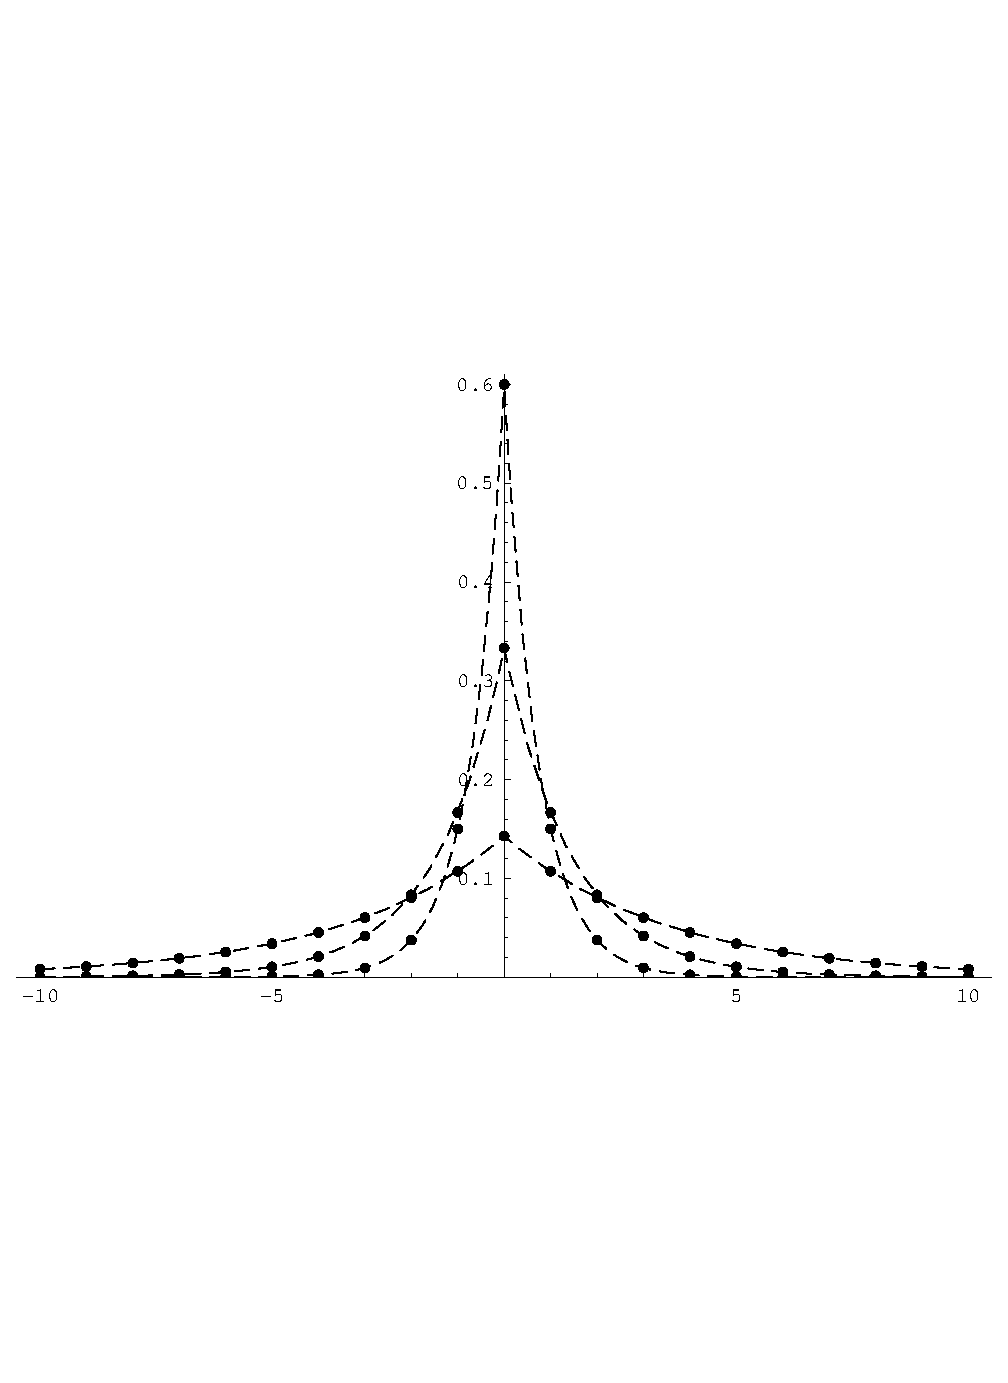
\includegraphics[width=\textwidth]{diffGeom.eps}
        \hfill
    }
    \vspace*{-30ex}
    \caption[Distribution of Discrete Random Numbers]{
        \label{verteilung}
        Distribution of Discrete Random Numbers
    }
\end{figure}

\subsection{Mutation Methods}

%---------------------------------------------------------------------------%
\index{mutateDiffGeom!( double s )}
\setNormalInstance
\printMethodWithOneParam
{void}
{mutateDiffGeom}
{double}
{s}
{Stepsize for the random number distribution.}
{A random number will be assigned to each allele of the chromosome 
 {\em this}. The method will use a special distribution with
 stepsize {\em s} for the random numbers.}
{None.}
{None.}
%---------------------------------------------------------------------------%

\clearpage

%---------------------------------------------------------------------------%
\index{mutateDiffGeom!( const vector$<$ double $>$\& s, bool cycle = false )}
\setNormalInstance
\setCorrectWidthThree{8pt}
\setParamOne{s}{const vector$<$ double $>$\&}{Vector that contains
stepsize values for each allele of {\em this}.
{\em s} should contain at most as many values as there are
alleles in {\em this}.
Otherwise the method will be aborted with an error
message.} 
\setParamTwo{cycle}{bool}{Specifies whether {\em s} can be used
circular ({\em cycle} = ``true'') or not ({\em cycle} = ``false'',
 this is the default).}
\printMethodWithParamsSaved
{void}
{}
{mutateDiffGeom}
{A random number will be assigned to each allele of the chromosome 
 {\em this}. The method will use a special distribution with
 a stepsize value for the random numbers. The vector {\em s}
 contains separate stepsize-values for each allele of {\em this}.
 As {\em s} can contain less values than {\em this} has alleles,
 the flag {\em cycle} can be used to specify whether {\em s}
 can be used circular or not.}
{}
\setCorrectWidthThree{4pt}
%---------------------------------------------------------------------------%

\vspace*{4ex}

%---------------------------------------------------------------------------%
\index{mutateDiffGeom!( const ChromosomeT$<$ double $>$\& s, bool cycle = false )}
\setNormalInstance
\setCorrectWidthThree{8pt}
\setParamOne{s}{const ChromosomeT$<$ double $>$\&}{See above.}
\setParamTwo{cycle}{bool}{See above.}
\printMethodWithParamsSaved
{void}
{}
{mutateDiffGeom}
{Same as above, but the stepsize values are saved in a {\tt double}
 chromosome.}
{}
\setCorrectWidthThree{4pt}
%---------------------------------------------------------------------------%

\clearpage

%---------------------------------------------------------------------------%
\index{mutateDiffGeom!( const Chromosome\& s, bool cycle = false )}
\setNormalInstance
\setCorrectWidthThree{8pt}
\setParamOne{s}{const Chromosome\&}{See above.}
\setParamTwo{cycle}{bool}{See above.}
\printMethodWithParamsSaved
{void}
{}
{mutateDiffGeom}
{Same as above, but the stepsize values are saved in a chromosome.}
{}
\setCorrectWidthThree{4pt}
%---------------------------------------------------------------------------%












%************************************************************************
% Class ChromosomeT< double >
%************************************************************************
\clearpage
\chapter{Class {\tt ChromosomeT$<$ double $>$}}
\index{ChromosomeT$<$ double $>$}

%------------------------------
% Abstract
%------------------------------
\section{Abstract}

This class contains methods and data structures for the work
with chromosomes of the numeric {\tt double} type and
is based upon the more general {\tt Chromosome} and 
{\tt ChromosomeT\_num} classes.
This also means, that all methods in these classes, which are
described in the corresponding references, can be used by
chromosomes of type {\tt double}, too.
This reference will describe all aditional methods, that
are available only for {\tt double} chromosomes, especially
methods that are used for structure optimization.
In the descriptions of the single methods the current instance
of class {\tt ChromosomeT$<$\nolinebreak\ double $>$}
will always be denoted as {\em this} (as it is usual in \cpp).


%------------------------------
% Internal Class DerandomConst
%------------------------------
\section{Internal Class {\em DerandomConst}}

The class {\tt ChromosomeT$<$ double $>$} contains an internal
subclass, that is used for the execution of the self-adaptative
method {\em Derandom}. The variables and methods that are
part of the subclass can not be called and modified directly, but
the {\tt ChromosomeT$<$ double $>$} class owns some methods for this
purpose. 

\subsection{Internal Variables of {\em DerandomConst}}

\begin{itemize}
\item {\em dim} - 
 Dimension of the chromosome. Not initialized. 
\index{dim (Variable)}

\item {\em C} -
 Period of cumulation, initialized with $\frac{1.0}{\sqrt{n}}$.
\index{C (Variable)}

\item {\em Cu} -
 Normalizing factor for the sum vector {\em s}, initialized with 
 $\sqrt{\frac{2.0 - C}{C}}$.
\index{Cu (Variable)}

\item {\em Crr} -
 Period of cumulation for the preference direction, initialized with 
 $\frac{3.0}{n}$. 
\index{Crr (Variable)}

\item {\em Beta} -
 Damping of the global stepsize adaptation, initialized 
 with $\frac{1.0}{\sqrt{n}}$.
\index{Beta (Variable)}

\item {\em BetaI} -
 Damping of the individual stepsize adaptation, initialized with
 $\frac{1}{n}$.
\index{BetaI (Variable)}

\item {\em BetaR} -
 Damping of the direction, initialized with $\frac{1.0}{\sqrt{4n}}$. 
\index{BetaR (Variable)}

\item {\em ChiN} -
 Expectation value for the $\chi_n$-distribution,\\ initialized with
 $\sqrt{n}(1 - \frac{1}{4n} + \frac{1}{21n^2})$.
\index{ChiN (Variable)}

\item {\em Chi1} -
 Expectation value for the $\chi_1$-distribution, initialized with
 $\sqrt{\frac{2}{\pi}}$.
\index{Chi1 (Variable)}

\end{itemize}

\clearpage

\subsection{Internal Methods of {\em DerandomConst}}

%---------------------------------------------------------------------------%
\index{DerandomConst!( unsigned n )}
\setNormalInstance
\printMethodWithOneParam
{}
{DerandomConst}
{unsigned}
{n}
{Initializing value for the dimension.}
{Initializes the internal variables of class {\em DerandomConst}.}
{None.}
{None.}
%---------------------------------------------------------------------------%

\vspace*{4ex}

%---------------------------------------------------------------------------%
\index{nobj!( )}
\setNormalInstance
\printEmptyMethodReturn
{unsigned}
{nobj}
{Returns the dimension value.}
{The dimension value.}
%---------------------------------------------------------------------------%

\vspace*{4ex}

%---------------------------------------------------------------------------%
\index{npar!( )}
\setNormalInstance
\printEmptyMethodReturn
{unsigned}
{npar}
{Returns the number of necessary parameters for the {\em Derandom} method.}
{Number of necessary parameters.}
%---------------------------------------------------------------------------%







%------------------------------
% Public Methods
%------------------------------
\clearpage
\section{Public Methods}

This methods can be used by all \cpp\ -programs, that have included
the header file {\em ChromosomeT.h} and the library {\em EA}.

%--------------------------------------------------------------------
% Initializing Methods
%--------------------------------------------------------------------
\vspace*{4ex}
\subsection{Initializing Methods}

These methods correspond to the methods described in the
section ``Self Adaptative Methods''.

\vspace*{2ex}

%---------------------------------------------------------------------------%
\index{initializeRotate!( double SigmaMin, double SigmaMax )}
\setNormalInstance
\setCorrectWidthThree{8pt}
\setParamOne{SigmaMin}{double}{Minimum possible random value.} 
\setParamTwo{SigmaMax}{double}{Maximum possible random value.}
\printMethodWithParamsSaved
{void}
{}
{initializeRotate}
{Initializes the strategy parameters (that means the alleles of
 {\em this}) for the method {\em mutateRotate} (see below) with
 normally distributed random values.}
{}
\setCorrectWidthThree{4pt}
%---------------------------------------------------------------------------%

\vspace*{4ex}

%---------------------------------------------------------------------------%
\index{initializeRotate!( const vector$<$ double $>$\& sigma )}
\setNormalInstance
\printMethodWithOneParam
{void}
{initializeRotate}
{const vector$<$ double $>$ \&}
{sigma}
{Vector containing initializing values for {\em this}.}
{Initializes the strategy parameters (that means the alleles of
 {\em this}) for the method {\em mutateRotate} (see below) with
 values contained in vector {\em sigma}.}
{None.}
{None.}
%---------------------------------------------------------------------------%

\clearpage

%---------------------------------------------------------------------------%
\index{initializeRotate!( const ChromosomeT$<$ double $>$\& sigma )}
\setNormalInstance
\printMethodWithOneParam
{void}
{initializeRotate}
{const ChromosomeT$<$ double $>$ \&}
{sigma}
{Chromosome containing initializing values for {\em this}.}
{Same as above, but here a chromosome is used to store the
 initializing values.}
{Keiner.}
{Keine.}
%---------------------------------------------------------------------------%

\vspace*{4ex}

%---------------------------------------------------------------------------%
\index{initializeDerandom!( double minVal, double maxVal )}
\setNormalInstance
\setCorrectWidthThree{8pt}
\setParamOne{minVal}{double}{Lower boundary of the random values interval.}
\setParamTwo{maxVal}{double}{Upper boundary of the random values interval.}
\printMethodWithParamsSaved
{void}
{}
{initializeDerandom}
{Initializes the strategy parameters (i.e. the alleles of
 {\em this}) for the method {\em mutateDerandom} (see below) with
 equally distributed random values.}
{Chromosome {\em this} must contain at least 5 alleles, otherwise
 the method will be aborted with an error message.}
\setCorrectWidthThree{4pt}
%---------------------------------------------------------------------------%

\vspace*{4ex}

%---------------------------------------------------------------------------%
\index{initializeCMA!( double SigmaMin, double SigmaMax )}
\setNormalInstance
\setCorrectWidthThree{8pt}
\setParamOne{SigmaMin}{double}{Minimum possible random value for the first
allele of {\em this}.}
\setParamTwo{SigmaMax}{double}{Maximum possible random value for the first
allele of {\em this}.}
\printMethodWithParamsSaved
{void}
{}
{initializeCMA}
{Initializes the strategy parameters (i.e. the alleles of
 {\em this}) for the method {\em mutateCMA} (see below).}
{}
\setCorrectWidthThree{4pt}
%---------------------------------------------------------------------------%

\clearpage

%---------------------------------------------------------------------------%
\index{initializeCMA!( const vector$<$ double $>$\& sigma )}
\setNormalInstance
\printMethodWithOneParam
{void}
{initializeCMA}
{const vector$<$ double $>$ \&}
{sigma}
{Vector containing initializing values for {\em this}.}
{Initializes the strategy parameters (i.e. the alleles of
 {\em this}) for the method {\em mutateCMA} (see below) with 
 values contained in vector {\em sigma}.}
{None.}
{None.}
%---------------------------------------------------------------------------%

\vspace*{4ex}

%---------------------------------------------------------------------------%
\index{initializeCMA!( const ChromosomeT$<$ double $>$\& sigma )}
\setNormalInstance
\printMethodWithOneParam
{void}
{initializeCMA}
{const ChromosomeT$<$ double $>$ \&}
{sigma}
{Chromosome containing the initializing values for {\em this}.}
{Same as above, but here a chromosome is used to store
 the initializing values.}
{Keiner.}
{Keine.}
%---------------------------------------------------------------------------%

\vspace*{4ex}

%---------------------------------------------------------------------------%
\index{initializeGSA!( double SigmaMin, double SigmaMax )}
\setNormalInstance
\setCorrectWidthThree{8pt}
\setParamOne{SigmaMin}{double}{Minimum possible random value for the first
allele of {\em this}.}
\setParamTwo{SigmaMax}{double}{Maximum possible random value for the first allele of {\em this}.}
\setParamThree{baseSize}{int}{Number of vectors of the
 generating set, ranging from $n^2$ to $2n^2$ ($n\ =\ $ number of
 alleles in {\em this}).}
\printMethodWithParamsSaved
{void}
{}
{initializeGSA}
{Initializes the strategy parameters (i.e. the alleles of
 {\em this}) for the method {\em mutateGSA} (see below).}
{}
\setCorrectWidthThree{4pt}
%---------------------------------------------------------------------------%

\clearpage

%---------------------------------------------------------------------------%
\index{initializeGSA!( const vector$<$ double $>$\& sigma, int baseSize )}
\setNormalInstance
\setCorrectWidthThree{8pt}
\setParamOne{sigma}{const vector$<$ double $>$ \&}{Vector containing
 initializing values for {\em this}.}
\setParamTwo{baseSize}{int}{Number of vectors of the
 generating set, ranging from $n^2$ to $2n^2$ ($n\ =\ $ number of
 alleles in {\em this}).}
\printMethodWithParamsSaved
{void}
{}
{initializeGSA}
{Initializes the strategy parameters (i.e. the alleles of
 {\em this}) for the method {\em mutateGSA} (see below) using
 values contained in vector {\em sigma}.}
{}
\setCorrectWidthThree{4pt}
%---------------------------------------------------------------------------%

\vspace*{4ex}

%---------------------------------------------------------------------------%
\index{initializeGSA!( const ChromosomeT$<$ double $>$\& sigma, int baseSize )}
\setNormalInstance
\setCorrectWidthThree{8pt}
\setParamOne{sigma}{const ChromosomeT$<$ double $>$ \&}{Chromosome containing
 the initializing values for {\em this}.}
\setParamTwo{baseSize}{int}{See above.}
\printMethodWithParamsSaved
{void}
{}
{initializeGSA}
{Same as above, but here a chromosome is used to store the
 initializing values for {\em this}.}
{}
\setCorrectWidthThree{4pt}
%---------------------------------------------------------------------------%

\vspace*{4ex}

%---------------------------------------------------------------------------%
\index{initializeIDA!( double SigmaMin, double SigmaMax )}
\setNormalInstance
\setCorrectWidthThree{8pt}
\setParamOne{SigmaMin}{double}{Minimum possible random value for several
  alleles of {\em this}.}
\setParamTwo{SigmaMax}{double}{Maximum possible random value for several
  alleles of {\em this}.}
\printMethodWithParamsSaved
{void}
{}
{initializeIDA}
{Initializes the strategy parameters (i.e. the alleles of
 {\em this}) for the method {\em mutateIDA} (see below).}
{}
\setCorrectWidthThree{4pt}
%---------------------------------------------------------------------------%

\clearpage

%---------------------------------------------------------------------------%
\index{initializeIDA!( const vector$<$ double $>$\& sigma )}
\setNormalInstance
\printMethodWithOneParam
{void}
{initializeIDA}
{const vector$<$ double $>$ \&}
{sigma}
{Vector containing initializing values for {\em this}.}
{Initializes the strategy parameters (i.e. the alleles of
 {\em this}) for the method {\em mutateIDA} (see below) using
 values contained in vector {\em sigma}.}
{None.}
{None.}
%---------------------------------------------------------------------------%

\vspace*{4ex}

%---------------------------------------------------------------------------%
\index{initializeIDA!( const ChromosomeT$<$ double $>$\& sigma )}
\setNormalInstance
\printMethodWithOneParam
{void}
{initializeIDA}
{const ChromosomeT$<$ double $>$ \&}
{sigma}
{Chromosome containing the initializing values for {\em this}.}
{Same as above, but here a chromosome is used to store the
 initializing values for {\em this}.}
{None.}
{None.}
%---------------------------------------------------------------------------%

\vspace*{4ex}

%---------------------------------------------------------------------------%
\index{initializeIDAiso!( double SigmaMin, double SigmaMax )}
\setNormalInstance
\setCorrectWidthThree{8pt}
\setParamOne{SigmaMin}{double}{Minimum possible random value for several
 alleles of {\em this}.}
\setParamTwo{SigmaMax}{double}{Maximum possible random value for several
 alleles of {\em this}.}
\printMethodWithParamsSaved
{void}
{}
{initializeIDAiso}
{Initializes the strategy parameters (i.e. the alleles of
 {\em this}) for the method {\em mutateIDAiso} (see below).}
{}
\setCorrectWidthThree{4pt}
%---------------------------------------------------------------------------%

\vspace*{4ex}

%---------------------------------------------------------------------------%
\index{initializeIDAiso!( const vector$<$ double $>$\& sigma )}
\setNormalInstance
\printMethodWithOneParam
{void}
{initializeIDAiso}
{const vector$<$ double $>$ \&}
{sigma}
{Vector containing initializing values for {\em this}.}
{Initializes the strategy parameters (i.e. the alleles of
 {\em this}) for the method {\em mutateIDAiso} (see below) using
 values contained in vector {\em sigma}.}
{None.}
{None.}
%---------------------------------------------------------------------------%

\clearpage

%---------------------------------------------------------------------------%
\index{initializeIDAiso!( const ChromosomeT$<$ double $>$\& sigma )}
\setNormalInstance
\printMethodWithOneParam
{void}
{initializeIDAiso}
{const ChromosomeT$<$ double $>$ \&}
{sigma}
{Chromosome with initializing values for {\em this}.}
{Same as above, but here a chromosome is used to store the
 initializing values for {\em this}.}
{Keiner.}
{Keine.}
%---------------------------------------------------------------------------%











%--------------------------------------------------------------------
% Decoding Method
%--------------------------------------------------------------------
\vspace*{4ex}
\subsection{Decoding Method}

%---------------------------------------------------------------------------%
\index{decodeBinary!( const Chromosome\& chrom, const Interval\& range, unsigned nbits, bool useGray = false )}
\setNormalInstance
\setCorrectWidthThree{8pt}
\setParamOne{chrom}{const Chromosome\&}{Chromosome that contains
the bitstring of decoded double values. The number of alleles of
{\em chrom} must be a multiple of {\em nbits}, otherwise
the method will be aborted with an error message.}
\setParamTwo{range}{const Interval\&}{values $\in [${\em range}$]$y}
\setParamThree{nbits}{unsigned}{Number of bits that were used for the decoding
of a single double value.}
\setParamFour{useGray}{bool}{Specifies, whether the double values were
decoded with the Gray method ({\em useGray} = "true") or the standard
method ({\em useGray} = "false", this is also the default).}
\printMethodWithParamsSaved
{void}
{}
{decodeBinary}
{Decodes several double values out of the interval {\em range}
 that are decoded as a bitstring and stored in chromosome {\em chrom}
 and stores them in {\em this}. For the decoding of each value 
 {\em nbits} bits were used. {\em useGray} specifies, whether
 the Gray method was used to decode the values or not.}
{}
\setCorrectWidthThree{4pt}
%---------------------------------------------------------------------------%


%--------------------------------------------------------------------
% Cumulation Methods
%--------------------------------------------------------------------
\clearpage
\subsection{Cumulation Methods}

%---------------------------------------------------------------------------%
\index{accumulate!( const vector$<$ double $>$\& acc, double c )}
\setNormalInstance
\setCorrectWidthThree{8pt}
\setParamOne{acc}{const vector$<$ double $>$ \&}{Vector that contains
the values to be added to the alleles of {\em this}.
{\em acc} must contain as many values as there are alleles in {\em this}.
 Otherwise the method will be aborted with an error message.}
\setParamTwo{c}{double}{Weighting factor for the values contained
in {\em acc}.}
\printMethodWithParamsSaved
{void}
{}
{accumulate}
{Adds the values contained in {\em acc} with weight {\em c} to
 the corresponding alleles of {\em this}.}
{}
\setCorrectWidthThree{4pt}
%---------------------------------------------------------------------------%

\vspace*{4ex}

%---------------------------------------------------------------------------%
\index{accumulate!( const Chromosome\& acc, double c )}
\setNormalInstance
\setCorrectWidthThree{8pt}
\setParamOne{acc}{const Chromosome \&}{See above.}
\setParamTwo{c}{double}{See above.}
\printMethodWithParamsSaved
{void}
{}
{accumulate}
{Same as above, but here a chromosome is used to store 
 the values to be added to the alleles of {\em this}.}
{}
\setCorrectWidthThree{4pt}
%---------------------------------------------------------------------------%







%--------------------------------------------------------------------
% Mutation Methods
%--------------------------------------------------------------------
\vspace*{4ex}
\subsection{Mutation Methods}

%---------------------------------------------------------------------------%
\index{mutateNormal!( double stddev )}
\setNormalInstance
\printMethodWithOneParam
{void}
{mutateNormal}
{double}
{stddev}
{Standard deviation for normally distributed random values.}
{Mutates all alleles of {\em this} by adding a normally distributed
 random value between "0" and the standard deviation {\em stddev}
 to the allele value.}
{None.}
{None.}
%---------------------------------------------------------------------------%

\clearpage

%---------------------------------------------------------------------------%
\index{mutateNormal!( const vector$<$ double $>$\& stddev, bool cycle )}
\setNormalInstance
\setCorrectWidthThree{8pt}
\setParamOne{stddev}{const vector$<$ double $>$ \&}{Vector that
contains standard deviation values for the single alleles of {\em this}.
{\em stddev} should contain at most as many values as there are
alleles in {\em this}. Otherwise the method will be aborted with an error
message.}
\setParamTwo{cycle}{bool}{Specifies, whether {\em stddev} can be
used circular ({\em cycle} = "true") or not ({\em cycle} = "false",
this is also the default).}
\printMethodWithParamsSaved
{void}
{}
{mutateNormal}
{Same as above, but here vector {\em stddev} contains a
 standard deviation value for each single allele of {\em this}.
 As {\em stddev} can contain less values than there are alleles in 
 {\em this}, the flag {\em cycle} denotes, whether {\em cycle}
 can be used circular or not.}
{}
\setCorrectWidthThree{4pt}
%---------------------------------------------------------------------------%

\vspace*{4ex}

%---------------------------------------------------------------------------%
\index{mutateNormal!( const Chromosome\& stddev, bool cycle )}
\setNormalInstance
\setCorrectWidthThree{8pt}
\setParamOne{stddev}{const Chromosome \&}{See above.}
\setParamTwo{cycle}{bool}{See above.}
\printMethodWithParamsSaved
{void}
{}
{mutateNormal}
{Same as above, but here a chromosome is used to store the
 standard deviation values.}
{}
\setCorrectWidthThree{4pt}
%---------------------------------------------------------------------------%

\vspace*{4ex}

%---------------------------------------------------------------------------%
\index{mutateNormal!( const ChromosomeT$<$ double $>$\& stddev, bool cycle )}
\setNormalInstance
\setCorrectWidthThree{8pt}
\setParamOne{stddev}{const ChromosomeT$<$ double $>$\&}{See above.}
\setParamTwo{cycle}{bool}{See above.}
\printMethodWithParamsSaved
{void}
{}
{mutateNormal}
{Same as above, but here a {\tt double} chromosome is used to store
 the standard deviation values.}
{}
\setCorrectWidthThree{4pt}
%---------------------------------------------------------------------------%

\clearpage

%---------------------------------------------------------------------------%
\index{mutateCauchy!( double scale )}
\setNormalInstance
\printMethodWithOneParam
{void}
{mutateCauchy}
{double}
{scale}            
{Scaling value for the random numbers.}
{Mutates all alleles of {\em this} by adding random numbers
 produced by the Cauchy method to the allele values. The random
 numbers will be scaled with {\em scale}.}
{None.}
{None.}
%---------------------------------------------------------------------------%

\vspace*{4ex}

%---------------------------------------------------------------------------%
\index{mutateCauchy!( const vector$<$ double $>$\& scale, bool cycle = false )}
\setNormalInstance
\setCorrectWidthThree{8pt}
\setParamOne{scale}{const vector$<$ double $>$\&}{Vector with scaling
values for each allele of {\em this}. {\em scale} must contain at most
as many values as there are alleles in {\em this}. Otherwise the method 
will be
aborted with an error message.}
\setParamTwo{cycle}{bool}{Specifies, whether {\em scale} can be used
circular ({\em cycle} = ``true'') or not ({\em cycle} = ``false'').}
\printMethodWithParamsSaved
{void}
{}
{mutateCauchy}
{Same as above, but here every allele of {\em this} has its own
 corresponding scaling value. These values are stored in vector {\em scale}.
 As {\em scale} can contain less values than there are alleles in {\em this},
 the flag {\em cycle} specifies, whether {\em scale} can be used
 circular or not.} 
{}
\setCorrectWidthThree{4pt}
%---------------------------------------------------------------------------%

\vspace*{4ex}

%---------------------------------------------------------------------------%
\index{mutateCauchy!( const Chromosome\& scale, bool cycle = false )}
\setNormalInstance
\setCorrectWidthThree{8pt}
\setParamOne{scale}{const Chromosome\&}{See above.}
\setParamTwo{cycle}{bool}{See above.}
\printMethodWithParamsSaved
{void}
{}
{mutateCauchy}
{Same as above, but here a chromosome is used to store the scaling
 values for the alleles of {\em this}.}
{}
\setCorrectWidthThree{4pt}
%---------------------------------------------------------------------------%

\clearpage

%---------------------------------------------------------------------------%
\index{mutateCauchy!( const ChromosomeT$<$ double $>$\& scale, bool cycle = false )}
\setNormalInstance
\setCorrectWidthThree{8pt}
\setParamOne{scale}{const ChromosomeT$<$ double $>$\&}{See above.}
\setParamTwo{cycle}{bool}{See above.}
\printMethodWithParamsSaved
{void}
{}
{mutateCauchy}
{Same as above, but here a {\tt double} chromosome is used to
 store the scaling values for the alleles of {\em this}.}
{}
\setCorrectWidthThree{4pt}
%---------------------------------------------------------------------------%











%--------------------------------------------------------------------
% Recombination Methods
%--------------------------------------------------------------------
\vspace*{4ex}
\subsection{Recombination Methods}

%---------------------------------------------------------------------------%
\index{recombineIntermediate!( const Chromosome\& dadChrom, const Chromosome\& momChrom )}
\setNormalInstance
\setCorrectWidthThree{8pt}
\setParamOne{dadChrom}{const Chromosome\&}{Father chromosome 
used for the recombination. Must contain as many alleles as {\em momChrom},
otherwise the method will be aborted with an error message.}
\setParamTwo{momChrom}{const Chromosome\&}{Mother chromosome 
used for the recombination. Must contain as many alleles as {\em dadChrom},
otherwise the method will be aborted with an error message.}
\printMethodWithParamsSaved
{void}
{}
{recombineIntermediate}
{Recombines {\em dadChrom} and {\em momChrom} with the intermediate method, 
 i.e. one allele
 of {\em this} will be assigned the average of the corresponding
 alleles of the parent chromosomes. The size of {\em this} will be
 adapted to the size of the parent chromosomes.}
{}
\setCorrectWidthThree{4pt}
%---------------------------------------------------------------------------%

\clearpage

%---------------------------------------------------------------------------%
\index{recombineGenIntermediate!( const Chromosome\& dadChrom, const Chromosome\& momChrom )}
\setNormalInstance
\setCorrectWidthThree{8pt}
\setParamOne{dadChrom}{const Chromosome\&}{See above.}
\setParamTwo{momChrom}{const Chromosome\&}{See above.}
\printMethodWithParamsSaved
{void}
{}
{recombineGenIntermediate}
{Recombines {\em dadChrom} and
 {\em momChrom} with the generalized intermediate method, i.e.
 one allele of {\em this} will be assigned an equally distributed
 random number, which value is between the value of the corresponding
 alleles of the parent chromosomes. The size of {\em this} will be
 adapted to the size of the parent chromosomes.}
{}
\setCorrectWidthThree{4pt}
%---------------------------------------------------------------------------%

\vspace*{4ex}

%---------------------------------------------------------------------------%
\index{recombineGeomIntermediate!( const Chromosome\& dadChrom, const Chromosome\& momChrom )}
\setNormalInstance
\setCorrectWidthThree{8pt}
\setParamOne{dadChrom}{const Chromosome\&}{See above.}
\setParamTwo{momChrom}{const Chromosome\&}{See above.}
\printMethodWithParamsSaved
{void}
{}
{recombineGeomIntermediate}
{Recombines {\em dadChrom} and
 {\em momChrom} with the geometric intermediate method, i.e.
 one allele of {\em this} will be assigned the square root of the
 product of the corresponding alleles of the parent chromosomes i.e.
 $this_i = \sqrt{dadChrom_i \cdot momChrom_i}$ for an allele with index
 {\em i}. The size of {\em this} will be adapted to the size of 
 the parent chromosomes.}
{}
\setCorrectWidthThree{4pt}
%---------------------------------------------------------------------------%

\vspace*{4ex}

%---------------------------------------------------------------------------%
\index{recombineIntermediate!( Chromosome\& mate )}
\setNormalInstance
\printMethodWithOneParam
{void}
{recombineIntermediate}
{Chromosome\&}
{mate}
{Chromosome that will be recombined with {\em this}. {\em mate} must contain
 as many alleles as {\em this}, otherwise the method will be aborted with
 an error message.}
{Recombines the chromosomes {\em this} and {\em mate} by using the
 intermediate method, i.e. the old allele values of {\em this}
 will be replaced by the average of the corresponding alleles of {\em mate}
 and the old allele values of {\em this}.}
{None.}
{None.}
%---------------------------------------------------------------------------%

\clearpage

%---------------------------------------------------------------------------%
\index{recombineGenIntermediate!( Chromosome\& mate )}
\setNormalInstance
\printMethodWithOneParam
{void}
{recombineGenIntermediate}
{Chromosome\&}
{mate}
{See above.}
{Recombines the chromosomes {\em this} and {\em mate} by using the 
 generalized intermediate method, i.e. the old allele values of 
 {\em this}
 will be replaced by equally distributed random numbers between
 the average of the corresponding alleles of {\em mate}
 and the old allele values of {\em this}.}
{None.}
{None.}
%---------------------------------------------------------------------------%

\vspace*{4ex}

%---------------------------------------------------------------------------%
\index{recombineGeomIntermediate!( Chromosome\& mate )}
\setNormalInstance
\printMethodWithOneParam
{void}
{recombineGeomIntermediate}
{Chromosome\&}
{mate}
{See above.}
{Recombines the chromosomes {\em this} and {\em mate} by using the 
 geometric intermediate method, i.e. the old allele values of 
 {\em this}
 will be replaced by the square root of the product of the corresponding 
alleles of {\em mate}
 and the old allele values of {\em this}, i.e.
 $this_{i_{new}} = mate_{i_{new}} = \sqrt{this_{i_{old}} \cdot 
    mate_{i_{old}}}$ 
    for an allele with index {\em i}.}
{None.}
{None.}
%---------------------------------------------------------------------------%


%--------------------------------------------------------------------
% Self Adaptative Methods
%--------------------------------------------------------------------
\vspace*{4ex}
\subsection{Self Adaptative Methods}

%---------------------------------------------------------------------------%
\index{mutateLogNormal!( double overallStdDev, double indivStdDev )}
\setNormalInstance
\setCorrectWidthThree{8pt}
\setParamOne{overallStdDev}{double}{Standard deviation for the mutation
of the stepsize for all components of {\em this}.}
\setParamTwo{indivStdDev}{double}{Standard deviation for the mutation
of the stepsize for one component of {\em this}.}
\printMethodWithParamsSaved
{void}
{}
{mutateLogNormal}
{Mutates {\em this} by adding a normally distributed random number between
 ``0'' and $\sigma_i^2$ to each allele. The stepsize $\sigma_i$ will also
 be mutated for each component of {\em this} separately (parameter 
 {\em indivStdDev}) and for all components (parameter {\em overallStdDev}).
 For more information cf. \cite{EALibRef}, page 20.}
{}
\setCorrectWidthThree{4pt}
%---------------------------------------------------------------------------%

\clearpage

%---------------------------------------------------------------------------%
\index{mutateRotate!( ChromosomeT$<$ double $>$\& sigma )}
\setNormalInstance
\printMethodWithOneParam
{void}
{mutateRotate}
{ChromosomeT$<$ double $>$ \&}
{sigma}
{Chromosome with standard deviations for the normal distribution.}
{Mutates {\em this} and the strategy variables by using a
 rotation matrix. For more information cf.
 \cite{EALibRef}, p. 20 ff.}
{None.}
{None.}
%---------------------------------------------------------------------------%

\vspace*{4ex}

%---------------------------------------------------------------------------%
\index{mutateRotate!( ChromosomeT$<$ double $>$\& sigma, double tau1, double tau2, double beta, int sigmaCheck, double epsi )}
\setNormalInstance
\setCorrectWidthThree{8pt}
\setParamOne{sigma}{ChromosomeT$<$ double $>$\&}
{Chromosome with standard deviations for the normal distribution.}
\setParamTwo{tau1}{double}{Stepsize adaptation for all individuals.}
\setParamThree{tau2}{double}{Stepsize adaptation for one individual.}
\setParamFour{beta}{double}{Parameter $\beta$ for damping the
stepsize variation between successive generations.}
\setParamFive{sigmaCheck}{int}{If ``true''
check {\em sigma} for too small values.} 
\setParamSix{epsi}{double}{Lower boundary for the {\em sigma} values.}
\printMethodWithParamsSaved 
{void}
{}
{mutateRotate}
{Same as above, but with more parameters.}
{}
\setCorrectWidthThree{4pt}
%---------------------------------------------------------------------------%

\clearpage

%---------------------------------------------------------------------------%
\index{mutateNormalRotAngles!( const Chromosome\& sigma, const Chromosome\& alpha )}
\setNormalInstance
\setCorrectWidthThree{8pt}
\setParamOne{sigma}{const Chromosome\&}
{Chromosome with standard deviations for the normal distribution.}
\setParamTwo{alpha}{const Chromosome\&}
{Chromosome with anchor points for the rotations.}
\printMethodWithParamsSaved
{void}
{}
{mutateNormalRotAngles}
{Mutates {\em this} and the strategy variables by using a
 rotation matrix. For the rotations the rotation-anchor-points in
 {\em alpha} will be used. For more information cf.
 \cite{GSA}.}
{}
\setCorrectWidthThree{4pt}
%---------------------------------------------------------------------------%

\vspace*{4ex}

%---------------------------------------------------------------------------%
\index{mutateDerandom!( vector$<$ double $>$\& v, const DerandomConst\& K )}
\setNormalInstance
\setCorrectWidthThree{8pt}
\setParamOne{v}{vector$<$ double $>$\&}{Vector with parameter values for
the mutation method.}
\setParamTwo{K}{const DerandomConst\&}{Instance of the class 
{\em DerandomConst} with some constants for the mutation method.}
\printMethodWithParamsSaved
{void}
{}
{mutateDerandom}
{Mutates {\em this} by using the {\em Derandom} method. For more
 information cf. \cite{GSA}.}
{}
\setCorrectWidthThree{4pt}
%---------------------------------------------------------------------------%

\vspace*{4ex}

%---------------------------------------------------------------------------%
\index{mutateDerandom!( Chromosome\& chrom, const DerandomConst\& K )}
\setNormalInstance
\setCorrectWidthThree{8pt}
\setParamOne{chrom}{Chromosome\&}{Chromosome with parameter values for
the mutation method.}
\setParamTwo{K}{const DerandomConst\&}{See above.}
\printMethodWithParamsSaved
{void}
{}
{mutateDerandom}
{Same as above, but a chromosome is used to store the parameter
 values.}
{}
\setCorrectWidthThree{4pt}
%---------------------------------------------------------------------------%

\clearpage

%---------------------------------------------------------------------------%
\index{mutateCMA!( ChromosomeT$<$ double $>$\& sigma )}
\setNormalInstance
\printMethodWithOneParam
{void}
{mutateCMA}
{ChromosomeT$<$ double $>$ \&}
{sigma}
{Chromosome with standard deviations for the normal distribution.}
{Mutates {\em this} and the strategy parameters by using the mutation
 method with covariance matrix ({\em Covariance Matrix Adaptation}).
 For more information cf. \cite{CMA}.}
{None.}
{None.}
%---------------------------------------------------------------------------%

\vspace*{4ex}

%---------------------------------------------------------------------------%
\index{mutateCMA!( ChromosomeT$<$ double $>$\& sigma, double c, double cu, double ccov, double beta )}
\setNormalInstance
\setCorrectWidthThree{8pt}
\setParamOne{sigma}{ChromosomeT$<$ double $>$ \&}{Chromosome with standard 
deviations for the normal distribution.}
\setParamTwo{c}{double}{Value for determination of the cumulation
time for the sum vector {\em s}.}
\setParamThree{cu}{double}{Normalizes the variance of the sum vector {\em s}.}
\setParamFour{ccov}{double}{Time for the evaluation of the average
of the distribution $ss^t$ over the generation sequence.}
\setParamFive{beta}{double}{Parameter $\beta$ for damping the stepsize
varation between successive generations.}
\printMethodWithParamsSaved
{void}
{}
{mutateCMA}
{Same as above, but with more parameters.}
{}
\setCorrectWidthThree{4pt}
%---------------------------------------------------------------------------%

\vspace*{4ex}

%---------------------------------------------------------------------------%
\index{mutateMSR!( double xi\_prob )}
\setNormalInstance
\printMethodWithOneParam
{void}
{mutateMSR}
{double}
{xi\_prob}
{Probability to assign the value $\alpha = 1.5$ to the general
 stepsize variation factor $\xi$. The alternative value for
 $\xi$ is $\frac{1}{\alpha}$.}
{Mutates {\em this} and the strategy parameters by using the method
 with {\em mutative stepsize regulation}.
 For more information cf. \cite{MSR}.}
{None.}
{None.}
%---------------------------------------------------------------------------%

\clearpage

%---------------------------------------------------------------------------%
\index{mutateGSA!( ChromosomeT$<$ double $>$\& sigma )}
\setNormalInstance
\printMethodWithOneParam
{void}
{mutateGSA}
{ChromosomeT$<$ double $>$ \&}
{sigma}
{Chromosome with standard deviation for the normal distribution.}
{Mutates {\em this} and the strategy parameters by using the method
 with the {\em Generating Set Adaptation}.
 For more information cf. \cite{GSA}.}
{None.}
{None.}
%---------------------------------------------------------------------------%

\vspace*{4ex}

%---------------------------------------------------------------------------%
\index{mutateGSA!( ChromosomeT$<$ double $>$\& sigma, double beta, double xi\_const, double cu, double cm )}
\setNormalInstance
\setCorrectWidthThree{8pt}
\setParamOne{sigma}{ChromosomeT$<$ double $>$ \&}
{Chromosome with standard deviation for the normal distribution.}
\setParamTwo{beta}{double}{Parameter $\beta$ for damping the stepsize
variation between successive generations.}
\setParamThree{xi\_const}{double}{Factor for the stepsize adaptation.
Normally the values $1.5$ and $\frac{1}{1.5}$ will be assigned to 
{\em xi\_const} with the same probability. Here the factor can be
stated explicitly.}
\setParamFour{cu}{double}{Normalizing factor for the variances.}
\setParamFive{cm}{double}{Length adaptation factor.}
\printMethodWithParamsSaved
{void}
{}
{mutateGSA}
{Same as above, but with more parameters.} 
{}
\setCorrectWidthThree{4pt}
%---------------------------------------------------------------------------%

\vspace*{4ex}

%---------------------------------------------------------------------------%
\index{mutateIDA!( ChromosomeT$<$ double $>$\& sigma )}
\setNormalInstance
\printMethodWithOneParam
{void}
{mutateIDA}
{ChromosomeT$<$ double $>$ \&}
{sigma}
{Chromosome with standard deviations for the normal distribution.}
{Mutates {\em this} and the strategy parameters by using the {\em Individual 
 step sizes and one Direction Adaptation}.\\
 For more informations cf. \cite{EALibRef}, p. 22 ff.}
{None.}
{None.}
%---------------------------------------------------------------------------%

\clearpage

%---------------------------------------------------------------------------%
\index{mutateIDA!( ChromosomeT$<$ double $>$\& sigma, double c, double c\_r, double beta, double beta\_ind, double beta\_r, double cu, double xi )}
\setNormalInstance
\setCorrectWidthThree{8pt}
\setParamOne{sigma}{ChromosomeT$<$ double $>$ \&}
{Chromosome with standard deviations for the normal distribution.}
\setParamTwo{c}{double}{Defines the cumulation time.}
\setParamThree{c\_r}{double}{Also defines the cumulation time.}
\setParamFour{beta}{double}{Parameter $\beta$ for damping the stepsize
variation between successive generations.}
\setParamFive{beta\_ind}{double}{Parameter for damping the stepsize
variation between successive generations for one individual.}
\setParamSix{beta\_r}{double}{Parameter for damping the stepsize
variation between successive generations for the direction.}
\setParamSeven{cu}{double}{Normalizing factor for variances.}
\setParamEight{xi}{double}{Factor for the stepsize adaptation.
Normally the values $1.5$ and $\frac{1}{1.5}$ will be assigned to 
{\em xi} with the same probability. Here the factor can be stated
explicitly.}
\printMethodWithParamsSaved
{void}
{}
{mutateIDA}
{Same as above, but with more parameters.}
{}
\setCorrectWidthThree{4pt}
%---------------------------------------------------------------------------%

\vspace*{4ex}

%---------------------------------------------------------------------------%
\index{mutateIDAiso!( ChromosomeT$<$ double $>$\& sigma )}
\setNormalInstance
\printMethodWithOneParam
{void}
{mutateIDAiso}
{ChromosomeT$<$ double $>$ \&}
{sigma}
{Chromosome with standard deviations for the normal distribution.}
{This method does the same as {\em mutateIDA}, but here 
 no adaptation of the preference direction takes place.}
{Keiner.}
{Keine.}
%---------------------------------------------------------------------------%

\clearpage

%---------------------------------------------------------------------------%
\index{mutateIDAiso!( ChromosomeT$<$ double $>$\& sigma, double c, double beta, double beta\_ind, double cu )}
\setNormalInstance
\setCorrectWidthThree{8pt}
\setParamOne{sigma}{ChromosomeT$<$ double $>$ \&}
{Chromosome with standard deviations for the normal distribution.}
\setParamTwo{c}{double}{Defines the cumulation time.}
\setParamThree{beta}{double}{Parameter $\beta$ for damping the stepsize
variation between successive generations.}
\setParamFour{beta\_ind}{double}{Parameter for damping the stepsize
variation between successive generations for one individual.}
\setParamFive{cu}{double}{Normalizing factor for the variances.}
\printMethodWithParamsSaved
{void}
{}
{mutateIDAiso}
{Same as above, but with more parameters.}
{}
\setCorrectWidthThree{4pt}
%---------------------------------------------------------------------------%





%--------------------------------------------------------------------
% Methods for Displaying Parameters
%--------------------------------------------------------------------
\vspace*{4ex}
\subsection{Methods for Displaying Parameters}

%---------------------------------------------------------------------------%
\index{showRotate!( )}
\setNormalInstance
\printEmptyMethod
{showRotate}
{Displays the parameters {\em sigma} and {\em alpha} of the self adaptation
 method {\em mutateRotate} (see above).}
%---------------------------------------------------------------------------%

\vspace*{4ex}

%---------------------------------------------------------------------------%
\index{showCMA!( )}
\setNormalInstance
\printEmptyMethod
{showCMA}
{Displays the parameters of the self adaptation
 method {\em mutateCMA} (see above).}
%---------------------------------------------------------------------------%

\clearpage

%---------------------------------------------------------------------------%
\index{showIDA!( )}
\setNormalInstance
\printEmptyMethod
{showIDA}
{Displays the parameters of the self adaptation
 method {\em mutateIDA} (see above).}
%---------------------------------------------------------------------------%

\vspace*{4ex}

%---------------------------------------------------------------------------%
\index{showGSA!( int baseSize )}
\setNormalInstance
\printMethodWithOneParam
{void}
{showGSA}
{int}
{baseSize}
{Number of vectors of the generating set, ranging from $n^2$ to 
 $2n^2$ ($n\ =\ $ number of alleles in {\em this}).}
{Displays the parameters of the self adaptation
 method {\em mutateGSA} (see above).}
{None.}
{None.}
%---------------------------------------------------------------------------%

\vspace*{4ex}

%---------------------------------------------------------------------------%
\index{dumpDerandom!( ostream\& os )}
\setConstInstance
\printMethodWithOneParam
{void}
{dumpDerandom}
{ostream\&}
{os}
{Output stream to which the parameter values will be written.}
{Writes the parameter values of the {\em Derandom Self Adaptation} method
 (see above) to the output stream {\em os}.}
{None.}
{The chromosome {\em this} must contain at least 5 alleles, otherwise
 the method will be aborted with an error message.}
%---------------------------------------------------------------------------%











%************************************************************************
% Class Individual
%************************************************************************
\clearpage
\chapter{Class {\tt Individual}}
\index{Individual}

%------------------------------
% Abstract
%------------------------------
\section{Abstract}

This class contains methods and data structures for the work
with individuals of a population.\\
An individual consists of a specific number of chromosomes
of any type, the so called ``genome''. The single chromosomes
of an individual can be of different type.
Internally, an individual is stored as a vector of pointers
to several chromosomes.\\
In the descriptions of the single methods the current instance
of class {\tt Individual}
will always be denoted as {\em this} (as it is usual in \cpp).


%------------------------------
% Internal Variables & Flags
%------------------------------
\section{Internal Variables and Flags}

The class {\tt Individual} includes some internal variables and flags, that
are necessary for several methods.
To manipulate these data the class offers several methods.

\subsection{Internal Variables}

\begin{itemize}
\item {\em fitness} -
Result of the evaluation of an individual, will be initialized with
0.
\index{fitness (Variable)}

\item {\em scaledFitness} -
The value that will be produced by an evaluation function {\em f}
will always be mapped to a positive fitness value using a
scaling function. Additionally, the sum of the mapped fitness values of all
individuals of the parent population must be 1.0.
These normalized values are called scaled fitness values and when an
individual is generated, its corresponding scaled fitness value will be
initialized with 0.
\index{scaledFitness (Variable)}

\item {\em age} -
The age of the individual, will be initialized with 0.
\index{age (Variable)}

\item {\em selProb} - 
The selection probability of the individual. Defaults to zero. 
\index{selProb (Variable)}

\item {\em numCopies} -
Denotes the number of reproductions of the individual
during the last selection. This variable will be initialized
with 0.
\end{itemize}
\index{numCopies (Variable)}

\clearpage

\subsection{Internal Flags}

\begin{itemize}

\item {\em evalFlg} -
Denotes whether the fitness of the individual must be
evaluated (``true'') or not (``false'').
The flag will be initialized with ``false''.
\index{evalFlg (Variable)}

\item {\em feasible} -
Denotes whether the current individual is a possible
solution for the optimization problem (``true'') or
not (``false''). The flag will be initialized with ``false''.
\index{feasible (Variable)}

\item {\em elitist} -
Denotes whether the individual was selected as an elitist
during the last selection (``true'') or not (``false'').
The flag will be initialized with ``false''.
\end{itemize}
\index{elitist (Variable)}


%------------------------------
% Public Methods
%------------------------------
\section{Public Methods}

These methods can be used by all \cpp\ -programs that have included
the header file {\em Individual.h} and the library {\em EA}.

%-------------------------------------------------------------------
% Constructors
%-------------------------------------------------------------------
\vspace*{4ex}
\subsection{Constructors}

%---------------------------------------------------------------------------%
\index{Individual!( )}
\setNormalInstance
\printEmptyMethod
{Individual}
{Generates an empty individual.}
%---------------------------------------------------------------------------%

\vspace*{4ex}

%---------------------------------------------------------------------------%
\index{Individual!( unsigned n )}
\setNormalInstance
\printMethodWithOneParam
{explicit}
{Individual}
{unsigned}
{n}
{Number of chromosomes.}
{Generates a new individual and reserves memory for
 {\em n} chromosomes of type {\tt char}.}
{None.}
{{\em explicit} = Implicit calls of the constructor in assignments of type
 {\tt Individual} {\em ind} = $<$Value$>$ are not possible.}
%---------------------------------------------------------------------------%

\clearpage

%---------------------------------------------------------------------------%
\index{Individual!( unsigned n, const Chromosome\& chrom )}
\setNormalInstance
\setCorrectWidthThree{8pt}
\setParamOne{n}{unsigned}{Number of clones.}
\setParamTwo{chrom}{const Chromosome\&}{Chromosome to be cloned.}
\printMethodWithParamsSaved
{}
{}
{Individual}
{Generates an individual that consists of {\em n} clones of the
 chromosome {\em chrom}.}
{}
\setCorrectWidthThree{4pt}
%---------------------------------------------------------------------------%

\vspace*{4ex}

%---------------------------------------------------------------------------%
\index{Individual!( const Chromosome\& chrom0 )}
\setNormalInstance
\printMethodWithOneParam
{}
{Individual}
{const Chromosome\&}
{chrom0}
{Chromosome, to be cloned.}
{Generates an individual that consists of the chromosome {\em chrom0}.}
{None.}
{None.}
%---------------------------------------------------------------------------%

\vspace*{4ex}

%---------------------------------------------------------------------------%
\index{Individual!( const Chromosome\& chrom0, const Chromosome\& chrom1 )}
\setNormalInstance
\setCorrectWidthThree{8pt}
\setParamOne{chrom0}{const Chromosome\&}{First chromosome, which 
is part of the new individual.}
\setParamTwo{chrom1}{const Chromosome\&}{Second chromosome, which 
is part of the new individual.}
\printMethodWithParamsSaved
{}
{}
{Individual}
{Generates an individual that consists of the chromosomes {\em chrom0} 
 and {\em chrom1}.}
{}
\setCorrectWidthThree{4pt}
%---------------------------------------------------------------------------%

\clearpage

%---------------------------------------------------------------------------%
\index{Individual!( const Chromosome\& chrom0 .. chrom2 )}
\setNormalInstance
\printMethodWithOneParam
{}
{Individual}
{const Chromosome\&}
{chrom0 .. chrom2}
{Chromosomes that make up the new individual.}
{Generates an individual that consists of the chromosomes
 {\em chrom0} to {\em chrom2}.}
{None.}
{None.}
%---------------------------------------------------------------------------%

\vspace*{4ex}

%---------------------------------------------------------------------------%
\index{Individual!( const Chromosome\& chrom0 .. chrom3 )}
\setNormalInstance
\printMethodWithOneParam
{}
{Individual}
{const Chromosome\&}
{chrom0 .. chrom3}
{Chromosomes, that make up the new individual.}
{Generates an individual that consists of the chromosomes {\em chrom0}
 to {\em chrom3}.}
{None.}
{None.}
%---------------------------------------------------------------------------%

\vspace*{4ex}

%---------------------------------------------------------------------------%
\index{Individual!( const Chromosome\& chrom0 .. chrom4 )}
\setNormalInstance
\printMethodWithOneParam
{}
{Individual}
{const Chromosome\&}
{chrom0 .. chrom4}
{Chromosomes, that make up the new individual.}
{Generates an individual that consists of the chromosomes {\em chrom0} to
 {\em chrom4}.}
{None.}
{None.}
%---------------------------------------------------------------------------%

\clearpage

%---------------------------------------------------------------------------%
\index{Individual!( const Chromosome\& chrom0 .. chrom5 )}
\setNormalInstance
\printMethodWithOneParam
{}
{Individual}
{const Chromosome\&}
{chrom0 .. chrom5}
{Chromosomes, that make up the new individual.}
{Generates an individual that consist of the chromosomes {\em chrom0}
 to {\em chrom5}.}
{None.}
{None.}
%---------------------------------------------------------------------------%

\vspace*{4ex}

%---------------------------------------------------------------------------%
\index{Individual!( const Chromosome\& chrom0 .. chrom6 )}
\setNormalInstance
\printMethodWithOneParam
{}
{Individual}
{const Chromosome\&}
{chrom0 .. chrom6}
{Chromosomes, that make up the new individual.}
{Generates an individual that consist of the chromosomes {\em chrom0} to
 {\em chrom6}.}
{None.}
{None.}
%---------------------------------------------------------------------------%

\vspace*{4ex}

%---------------------------------------------------------------------------%
\index{Individual!( const Chromosome\& chrom0 .. chrom7 )}
\setNormalInstance
\printMethodWithOneParam
{}
{Individual}
{const Chromosome\&}
{chrom0 .. chrom7}
{Chromosomes, that make up the new individual.}
{Generates an individual that consist of the chromosomes {\em chrom0}
 to {\em chrom7}.}
{None.}
{None.}
%---------------------------------------------------------------------------%

\clearpage

%---------------------------------------------------------------------------%
\index{Individual!( const vector$<$ Chromosome$\ast$ $>$\& chrom )}
\setNormalInstance
\printMethodWithOneParam
{}
{Individual}
{const vector$<$ Chromosome* $>$\&}
{chrom}
{The vector of chromosomes.}
{Generates an individual that consists of the chromosomes stored in 
 vector {\em chrom}.}
{None.}
{None.}
%---------------------------------------------------------------------------%

\vspace*{4ex}

%---------------------------------------------------------------------------%
\index{Individual!( const Individual\& indiv )}
\setNormalInstance
\printMethodWithOneParam
{}
{Individual}
{const Individual\&}
{indiv}
{Individual.}
{Generates an individual that is a copy of {\em indiv} including
 the internal class variables.}
{None.}
{None.}
%---------------------------------------------------------------------------%


%-------------------------------------------------------------------
% Destructor
%-------------------------------------------------------------------
\vspace*{4ex}
\subsection{Destructor}

%---------------------------------------------------------------------------%
\index{$\sim$Individual!( )}
\printEmptyMethodReturnSpecial
{virtual}
{$\sim$Individual}
{Removes all chromosomes, that are contained in the individual {\em this}
 and then destroys {\em this} itself.}
{None.}
{This destructor is only virtual, its functionality can be inherited
 and expanded by the derived classes. The destructor should not
 be called directly.}
%---------------------------------------------------------------------------%


%-------------------------------------------------------------------
% Operators
%-------------------------------------------------------------------
\clearpage
\subsection{Operators}

\subsubsection{Assignment Operators}

%---------------------------------------------------------------------------%
\index{operator =!( onst Individual\& indiv )}
\setNormalInstance
\printMethodWithOneParam
{Individual\&}
{operator =\ }
{const Individual\&}
{indiv}
{Individual that will be assigned to {\em this}.}
{Assigns the individual {\em indiv} (i.e. the chromosomes that
 are contained in {\em indiv} and the values of the internal
 class variables) to {\em this}.}
{The individual {\em this} with its new values.}
{None.}
%---------------------------------------------------------------------------%

\subsubsection{Comparison Operators}

%---------------------------------------------------------------------------%
\index{operator ==!( const Individual\& ind )}
\setConstInstance
\printMethodWithOneParam
{bool}
{operator ==\ }
{const Individual\&}
{ind}
{Individual that will be compared with {\em this}.}
{Checks whether the current individual {\em this} and the
 individual {\em ind} are equal. The individuals are equal,
 if they contain the same number of chromosomes, if any
 chromosome of {\em this} is equal to its corresponding
 chromosome in {\em ind} and if all values of the internal
 class variables are equal.}
{
 {\em true}  - The individuals are equal,\\
 {\em false} - The individuals are not equal.}
{None.}
%---------------------------------------------------------------------------%

\vspace*{4ex}

%---------------------------------------------------------------------------%
\index{operator $<$!( const Individual\& ind )}
\setConstInstance
\printMethodWithOneParam
{bool}
{operator $<$\ }
{const Individual\&}
{ind}
{Individual that will be compared with {\em this}.}
{Checks whether the current individual {\em this} is less than
 the individual {\em ind}, i.e. whether {\em this}
 contains less chromosomes than {\em ind} or -- if both individuals
 have the same number of chromosomes -- at least one chromosome
 of {\em this} is less than its corresponding chromosome
 in {\em ind}.}
{
 {\em true}  - {\em this} is less than {\em ind},\\
 {\em false} - {\em this} is greater than {\em ind} or both individuals
 are equal.}
{None.}
%---------------------------------------------------------------------------%

\clearpage

%---------------------------------------------------------------------------%
\index{operator $>$!( const Individual\& ind )}
\setConstInstance
\printMethodWithOneParam
{bool}
{operator $>$\ }
{const Individual\&}
{ind}
{Individual that will be compared with {\em this}.}
{Checks whether the current individual {\em this} is greater than
 the individual {\em ind}, i.e. whether {\em this}
 contains more chromosomes than {\em ind} or -- if both individuals
 have the same number of chromosomes -- at least one chromosome
 of {\em this} is greater than its corresponding chromosome
 in {\em ind}.}
{
 {\em true}  - {\em this} is greater than {\em ind},\\
 {\em false} - {\em this} is less than {\em ind}, or both individuals
 are equal.}
{None.}
%---------------------------------------------------------------------------%

\vspace*{4ex}

%---------------------------------------------------------------------------%
\index{operator $<$=!( const Individual\& ind )}
\setConstInstance
\printMethodWithOneParam
{bool}
{operator $<=$\ }
{const Individual\&}
{ind}
{Individual that will be compared with {\em this}.}
{Checks whether the current individual {\em this} is less than
 the individual {\em ind} or whether both individuals are equal (see
 above).}
{
 {\em true}  - {\em this} is less than {\em ind} or both individuals
 are equal,\\
 {\em false} - {\em this} is greater than {\em ind}.}
{None.}
%---------------------------------------------------------------------------%

\vspace*{4ex}

%---------------------------------------------------------------------------%
\index{operator $>$=!( const Individual\& ind )}
\setConstInstance
\printMethodWithOneParam
{bool}
{operator $>=$\ }
{const Individual\&}
{ind}
{Individual that will be compared with {\em this}.} 
{Checks whether the current individual {\em this} is greater than
 the individual {\em ind} or whether both individuals are equal (see
 above).}
{
 {\em true}  - {\em this} greater than {\em ind} or both individuals
 are equal,\\ 
 {\em false} - {\em this} is less than {\em ind}.}
{None.}
%---------------------------------------------------------------------------%

\clearpage

%---------------------------------------------------------------------------%
\index{operator $\mid$=!( const Individual\& ind )}
\setConstInstance
\printMethodWithOneParam
{bool}
{operator $!=$\ }
{const Individual\&}
{ind}
{Individual that will be compared with {\em this}.} 
{Checks whether the current individual {\em this} and the
 individual {\em ind} are different, i.e. whether
 {\em this} is less or greater than {\em ind} (see above).}
{
 {\em true}  - {\em this} and {\em ind} are different,\\
 {\em false} - {\em this} and {\em ind} are equal.}
{None.}
%---------------------------------------------------------------------------%

\subsubsection{Operator for Extracting a Single Chromosome}

%---------------------------------------------------------------------------%
\index{operator [ ]!( unsigned i )}
\setNormalInstance
\printMethodWithOneParam
{Chromosome\&}
{operator [\ ]\ }
{unsigned}
{i}
{Index of the chromosome in {\em this}, to be returned.
 {\em i} must be less than the number of chromosomes in {\em this},
 otherwise the method will be aborted with an error message.}
{Returns the chromosome with index {\em i} in the individual {\em this}.}
{Chromosome with index {\em i}.}
{None.}
%---------------------------------------------------------------------------%






%-------------------------------------------------------------------
% Information Retrieval Methods
%-------------------------------------------------------------------
\clearpage
\subsection{Information Retrieval Methods}

%---------------------------------------------------------------------------%
\index{size!( )}
\setConstInstance
\printEmptyMethodReturn
{unsigned}
{size}
{Returns the number of chromosome in {\em this}.}
{Number of chromosomes in {\em this}.}
%---------------------------------------------------------------------------%

\vspace*{4ex}

%---------------------------------------------------------------------------%
\index{totalSize!( )}
\setConstInstance
\printEmptyMethodReturn
{unsigned}
{totalSize}
{Returns the number of all alleles of the chromosomes in {\em this}.}
{The whole number of alleles in {\em this}.}
%---------------------------------------------------------------------------%

\vspace*{4ex}

%---------------------------------------------------------------------------%
\index{fitnessValue!( )}
\setConstInstance
\printEmptyMethodReturn
{double}
{fitnessValue}
{Returns the fitness value of the current individual {\em this}.}
{Fitness value of {\em this}.}
%---------------------------------------------------------------------------%

\vspace*{4ex}

%---------------------------------------------------------------------------%
\index{getAge!( )}
\setConstInstance
\printEmptyMethodReturn
{unsigned}
{getAge}
{Returns the age of {\em this}, i.e. the generation {\em this} is from.}
{Age of {\em this}.}
%---------------------------------------------------------------------------%

\clearpage

%---------------------------------------------------------------------------%
\index{needEvaluation!( )}
\setConstInstance
\printEmptyMethodReturn
{bool}
{needEvaluation}
{Returns the status of the {\em evalFlg}, i.e. whether the individual must 
 be evaluated.}
{Status of {\em evalFlg}:\\
 {\em true} - An evaluation of {\em this} is necessary,\\
 {\em false} - The individual needs no evaluation.}
%---------------------------------------------------------------------------%

\vspace*{4ex}

%---------------------------------------------------------------------------%
\index{selectionProbability!( )}
\setConstInstance
\printEmptyMethodReturn
{double}
{selectionProbability}
{Returns the selection probability for {\em this}.}
{The selection probability of {\em this}.}
%---------------------------------------------------------------------------%

\vspace*{4ex}

%---------------------------------------------------------------------------%
\index{isFeasible!( )}
\setConstInstance
\printEmptyMethodReturn
{bool}
{isFeasible}
{Returns whether {\em this} is a possible solution for the
 current optimization problem.}
{Status of the {\em feasible}-flag:\\
 {\em true} - The individual is a possible solution,\\
 {\em false} - The individual cannot used as solution.}
%---------------------------------------------------------------------------%

\vspace*{4ex}

%---------------------------------------------------------------------------%
\index{numberOfCopies!( )}
\setConstInstance
\printEmptyMethodReturn
{unsigned}
{numberOfCopies}
{Returns the number of reproductions of {\em this} that occured
 during the last selection.}
{Number of reproductions of {\em this}.}
%---------------------------------------------------------------------------%

\clearpage

%---------------------------------------------------------------------------%
\index{isElitist!( )}
\setConstInstance
\printEmptyMethodReturn
{bool}
{isElitist}
{Returns the status of the {\em elitist}-flag, i.e. whether {\em this} 
 was chosen as elite individual during the last selection.}
{Status of the {\em elitist}-flag:\\
 {\em true} - The individual was chosen as elitist,\\
 {\em false} - The individual was not chosen.}
%---------------------------------------------------------------------------%



%-------------------------------------------------------------------
% Methods for Manipulating Internal Variables and Flags
%-------------------------------------------------------------------
\vspace*{4ex}
\subsection{Methods for Manipulating Internal Variables and Flags}

%---------------------------------------------------------------------------%
\index{setFitness!( double fit )}
\setNormalInstance
\printMethodWithOneParam
{void}
{setFitness}
{double}
{fit}
{New value for the normal and scaled fitness.}
{Sets the fitness and scaled fitness of {\em this} to the new
 value {\em fit}.}
{None.}
{None.}
%---------------------------------------------------------------------------%

\vspace*{4ex}

%---------------------------------------------------------------------------%
\index{setAge!( unsigned a )}
\setNormalInstance
\printMethodWithOneParam
{void}
{setAge}
{unsigned}
{a}
{New age of {\em this}. The default is 0.}
{Sets the age of {\em this} to the new value {\em a}.}
{None.}
{None.}
%---------------------------------------------------------------------------%

\vspace*{4ex}

%---------------------------------------------------------------------------%
\index{incAge!( )}
\setNormalInstance
\printEmptyMethod
{incAge}
{Increments the age of {\em this} by 1.}
%---------------------------------------------------------------------------%

\clearpage

%---------------------------------------------------------------------------%
\index{setEvaluationFlag!( )}
\setNormalInstance
\printEmptyMethod
{setEvaluationFlag}
{Sets {\em evalFlg} to ``true''.}
%---------------------------------------------------------------------------%

\vspace*{4ex}

%---------------------------------------------------------------------------%
\index{clearEvaluationFlag!( )}
\setNormalInstance
\printEmptyMethod
{clearEvaluationFlag}
{Sets {\em evalFlg} to ``false''.}
%---------------------------------------------------------------------------%

\vspace*{4ex}

%---------------------------------------------------------------------------%
\index{setFeasible!( bool f )}
\setNormalInstance
\printMethodWithOneParam
{void}
{setFeasible}
{bool}
{f}
{New value for the {\em feasible} flag:\\
{\em true} - The individual is a possible solution for the current
 optimization problem,\\
{\em false} - The individual does not represent a feasible solution.}
{Sets the {\em feasible} flag to the new value {\em f}.}
{None.}
{None.}
%---------------------------------------------------------------------------%

\vspace*{4ex}

%---------------------------------------------------------------------------%
\index{setSelectionProbability!( double ps )}
\setNormalInstance
\printMethodWithOneParam
{void}
{setSelectionProbability}
{double}
{ps}
{New selection probability for {\em this}.}
{Sets the selection probability of {\em this} to the new value {\em ps}.}
{None.}
{None.}
%---------------------------------------------------------------------------%






%-------------------------------------------------------------------
% Structure Changing Methods
%-------------------------------------------------------------------
\clearpage
\subsection{Structure Changing Methods}

%---------------------------------------------------------------------------%
\index{replace!( unsigned i, const Chromosome\& chrom )}
\setNormalInstance
\setCorrectWidthThree{8pt}
\setParamOne{i}{unsigned}{Index of the chromosome of {\em this}, to
be replaced. {\em i} must be less than the number of chromosomes
in {\em this}, otherwise the method will be aborted with an error message.}
\setParamTwo{chrom}{const Chromosome\&}{Chromosome that
replaces the old chromosome in {\em this}.}
\printMethodWithParamsSaved
{void}
{}
{replace}
{Replaces chromosome number {\em i} with the content of chromosome 
 {\em chrom}.}
{}
\setCorrectWidthThree{4pt}
%---------------------------------------------------------------------------%

\vspace*{4ex}

%---------------------------------------------------------------------------%
\index{insert!( unsigned i, const Chromosome\& chrom )}
\setNormalInstance
\setCorrectWidthThree{8pt}
\setParamOne{i}{unsigned}{Insertion-position in {\em this}.
The maximum value for {\em i} shall be equal to the
number of chromosomes in {\em this}, otherwise the method will be
aborted with an error message.}
\setParamTwo{chrom}{const Chromosome\&}{Chromosome to be inserted
into {\em this}.}
\printMethodWithParamsSaved
{void}
{}
{insert}
{Inserts chromosome {\em chrom} at position {\em i} into {\em this}.}
{}
\setCorrectWidthThree{4pt}
%---------------------------------------------------------------------------%

\vspace*{4ex}

%---------------------------------------------------------------------------%
\index{append!( const Chromosome\& chrom )}
\setNormalInstance
\printMethodWithOneParam
{void}
{append}
{const Chromosome\&}
{chrom}
{Chromosome to be appended at the end of {\em this}.}
{Appends the chromosome {\em chrom} at the end of {\em this}.}
{None.}
{None.}
%---------------------------------------------------------------------------%

\clearpage

%---------------------------------------------------------------------------%
\index{remove!( unsigned i )}
\setNormalInstance
\printMethodWithOneParam
{void}
{remove}
{unsigned}
{i}
{Index of the chromosome to be removed from {\em this}.
{\em i} must be less than the number of chromosomes in {\em this},
otherwise the method will be aborted with an error message.}
{Removes the chromosome with index {\em i} from {\em this}.}
{None.}
{None.}
%---------------------------------------------------------------------------%

\vspace*{4ex}

%---------------------------------------------------------------------------%
\index{remove!( unsigned from, unsigned to )}
\setNormalInstance
\setCorrectWidthThree{8pt}
\setParamOne{from}{unsigned}{Index of the first chromosome to be
removed. {\em from} must be less than the number of chromosomes in {\em this}
and not greater as {\em to} or the method will be aborted with an
error message.}
\setParamTwo{to}{unsigned}{Index of the last chromosome to be
removed. {\em to} must be less than the number of chromosomes in {\em this}
and not smaller as {\em from} or the method will be aborted with an
error message.}
\printMethodWithParamsSaved
{void}
{}
{remove}
{Removes all chromosomes with indices in the range $[from, to]$.}
{}
\setCorrectWidthThree{4pt}
%---------------------------------------------------------------------------%



%-------------------------------------------------------------------
% Input and Output Methods
%-------------------------------------------------------------------
\clearpage
\subsection{Input- and Output Methods}

%---------------------------------------------------------------------------%
\index{readFrom!( istream\& is )}
\setNormalInstance
\printMethodWithOneParam
{void}
{readFrom}
{istream\&}
{is}
{Input stream.}
{Replaces the data of {\em this} with the data read from the
 input stream {\em is}. The data must have the following format:\\
    ``{\tt Individual(}'',\\
    {\tt Size of the individual},\\ 
    ``{\tt )}'', Newline,\\ 
    {\tt Fitness value of the individual}, {\tt Newline},\\
    {\tt Scaled fitness value}, {\tt Newline},\\
    {\tt The value of {\em evalFlg}}, {\tt Newline},\\
    {\tt The value of the {\em feasible}-flag}, {\tt Newline},\\
    {\tt Selection probability of the individual}, {\tt Newline},\\
    {\tt Number of reproductions of the individual}, {\tt Newline},\\
    {\tt The value of the {\em elitist}-flag}, {\tt Newline},\\
    {\tt Age of the individual}, {\tt Newline},\\
    Then for each chromosome in the individual the following data:\\    
    ``{\tt ChromosomeT$<$}'',\\
    {\tt Type of the current chromosome},\\ 
    ``{\tt $>$(}'',\\ 
    {\tt Number of alleles of the current chromosome},\\
    ``{\tt )}'', {\tt Newline},\\
    {\tt The values of the single alleles of the current chromosome, separated by
    a space or a tab character}.}
{None.}
{None.}
%---------------------------------------------------------------------------%

\vspace*{4ex}

%---------------------------------------------------------------------------%
\index{writeTo!( ostream\& os )}
\setConstInstance
\printMethodWithOneParam
{void}
{writeTo}
{ostream\&}
{os}
{Ouput stream.}
{Writes all data of the individual {\em this} to the
 output stream {\em os}.}
{None.}
{None.}
%---------------------------------------------------------------------------%









%************************************************************************
% Class Population
%************************************************************************
\clearpage
\chapter{Class {\tt Population}}
\index{Population}

%------------------------------
% Abstract
%------------------------------
\section{Abstract}

This class contains methods and data structures for the work
with a population that consists of individuals.\\
Internally, a population is stored as a vector of pointers
to several individuals.\\
In the descriptions of the single methods the current instance
of class\\{\tt Population}
will always be denoted as {\em this} (as it is usual in \cpp).


%------------------------------
% Internal Variables & Flags
%------------------------------
\section{Internal Variables and Flags}

\subsection{Internal Variables}

\begin{itemize}

\index{index (Variable)}
\item {\em index} -
The index of the individual with the best fitness value in the
population. {\em index} will not be initialized.

\end{itemize}

\subsection{Internal Flags}

\begin{itemize}

\index{subPop (Variable)}
\item {\em subPop} -
Denotes whether the population is a subpopulation (``true'') or
not (``false''). A subpopulation can be generated when using
extinctive selection, where an individual can receive a
selection probability of zero. {\em subPop} will be initialized
with ``false''.

\index{ascending (Variable)}
\item {\em ascending} -
The individuals in the population are sorted according
to their fitness values. If the {\em ascending} flag is ``true'', the
individuals will be sorted by ascending fitness values, else by 
descending fitness values.
{\em ascending} will be initialized with ``false''.

\index{spinOnce (Variable)}
\item {\em spinOnce} -
In case {\em Roulette-Wheel-Selection} is 
used, the {\em spinOnce}-flag indicates whether the roulette
wheel will spin only one time (``true'') or several times
(``false''). The flag will be initialized with ``true''.
\end{itemize}


%------------------------------
% Public Methods
%------------------------------
\clearpage
\section{Public Methods}

These methods can be used by all \cpp\ -programs that have included
the header file {\em Population.h} and the library {\em EA}.

%--------------------------------------------------------------------
% Constructors
%--------------------------------------------------------------------
\vspace*{4ex}
\subsection{Constructors}

%---------------------------------------------------------------------------%
\index{Population!( )}
\setNormalInstance
\printEmptyMethod
{Population}
{Generates a new population.}
%---------------------------------------------------------------------------%

\vspace*{4ex}

%---------------------------------------------------------------------------%
\index{Population!( unsigned n )}
\setNormalInstance
\printMethodWithOneParam
{explicit}
{Population}
{unsigned}
{n}
{Number of individuals in the new population.}
{Generates a new population and reserves space for {\em n} individuals
 of undefined type.}
{None.}
{{\em explicit} = Implicit calls of the constructor using assignments of type
Population {\em pop} = $<$Value$>$ are not possible. This function is
not included in this version.}
%---------------------------------------------------------------------------%

\clearpage

%---------------------------------------------------------------------------%
\index{Population!( const Individual\& indiv )}
\setNormalInstance
\printMethodWithOneParam
{}
{Population}
{const Individual\&}
{indiv}
{Individual, that makes up the new population.}
{Generates a new population that consists of the individual {\em indiv}.}
{None.}
{None.}
%---------------------------------------------------------------------------%

\vspace*{4ex}

%---------------------------------------------------------------------------%
\index{Population!( unsigned n, const Individual\& indiv )}
\setNormalInstance
\setCorrectWidthThree{8pt}
\setParamOne{n}{unsigned}{Number of copies of {\em indiv}
to form the new population.}
\setParamTwo{indiv}{const Individual\&}{Individual.}
\printMethodWithParamsSaved
{}
{}
{Population}
{Generates a new population consisting of {\em n} copies of the
 individual {\em indiv}.}
{}
\setCorrectWidthThree{4pt}
%---------------------------------------------------------------------------%

\vspace*{4ex}

%---------------------------------------------------------------------------%
\index{Population!( unsigned n, const Chromosome\& chrom0 )}
\setNormalInstance
\setCorrectWidthThree{8pt}
\setParamOne{n}{unsigned}{Number of individuals that make up the new
population.}
\setParamTwo{chrom0}{const Chromosome\&}{Chromosome.}
\printMethodWithParamsSaved
{}
{}
{Population}
{Generates a new population consisting of {\em n} individuals that
 are formed by cloning chromosome {\em chrom0}.}
{}
\setCorrectWidthThree{4pt}
%---------------------------------------------------------------------------%

\clearpage

%---------------------------------------------------------------------------%
\index{Population!( unsigned n, const Chromosome\& chrom0, const Chromosome\& chrom1 )}
\setNormalInstance
\setCorrectWidthThree{8pt}
\setParamOne{n}{unsigned}{Number of individuals that make up the new
population.}
\setParamTwo{chrom0 .. chrom1}{const Chromosome\&}{Chromosomes to be cloned.}
\printMethodWithParamsSaved
{}
{}
{Population}
{Generates a new population that consists of {\em n} individuals
 formed by cloning the chromosomes {\em chrom0} and
 {\em chrom1}.}
{}
\setCorrectWidthThree{4pt}
%---------------------------------------------------------------------------%

\vspace*{4ex}

%---------------------------------------------------------------------------%
\index{Population!( unsigned n, const Chromosome\& chrom0 .. chrom2 )}
\setNormalInstance
\setCorrectWidthThree{8pt}
\setParamOne{n}{unsigned}{Number of individuals that make up the new
population.}
\setParamTwo{chrom0 .. chrom2}{const Chromosome\&}{Chromosomes to be 
cloned.}
\printMethodWithParamsSaved
{}
{}
{Population}
{Generates a new population that consists of {\em n} individuals
 formed by cloning the chromosomes {\em chrom0} to {\em chrom2}.}
{}
\setCorrectWidthThree{4pt}
%---------------------------------------------------------------------------%

\vspace*{4ex}

%---------------------------------------------------------------------------%
\index{Population!( unsigned n, const Chromosome\& chrom0 .. chrom3 )}
\setNormalInstance
\setCorrectWidthThree{8pt}
\setParamOne{n}{unsigned}{Number of individuals that make up the new
population.}
\setParamTwo{chrom0 .. chrom3}{const Chromosome\&}{Chromosomes to be 
cloned.}
\printMethodWithParamsSaved
{}
{}
{Population}
{Generates a new population that consists of {\em n} individuals
 formed by cloning the chromosomes {\em chrom0} to {\em chrom3}.}
{}
\setCorrectWidthThree{4pt}
%---------------------------------------------------------------------------%

\clearpage

%---------------------------------------------------------------------------%
\index{Population!( unsigned n, const Chromosome\& chrom0 .. chrom4 )}
\setNormalInstance
\setCorrectWidthThree{8pt}
\setParamOne{n}{unsigned}{Number of individuals that make up the new
population.}
\setParamTwo{chrom0 .. chrom4}{const Chromosome\&}{Chromosomes to be
cloned.}
\printMethodWithParamsSaved
{}
{}
{Population}
{Generates a new population that consists of {\em n} individuals
 formed by cloning the chromosomes {\em chrom0} to {\em chrom4}.}
{}
\setCorrectWidthThree{4pt}
%---------------------------------------------------------------------------%

\vspace*{4ex}

%---------------------------------------------------------------------------%
\index{Population!( unsigned n, const Chromosome\& chrom0 .. chrom5 )}
\setNormalInstance
\setCorrectWidthThree{8pt}
\setParamOne{n}{unsigned}{Number of individuals that make up the new
population.}
\setParamTwo{chrom0 .. chrom5}{const Chromosome\&}{Chromosomes to be
cloned.}
\printMethodWithParamsSaved
{}
{}
{Population}
{Generates a new population that consists of {\em n} individuals 
 formed by cloning the chromosomes {\em chrom0} to {\em chrom5}.}
{}
\setCorrectWidthThree{4pt}
%---------------------------------------------------------------------------%

\vspace*{4ex}

%---------------------------------------------------------------------------%
\index{Population!( unsigned n, const Chromosome\& chrom0 .. chrom6 )}
\setNormalInstance
\setCorrectWidthThree{8pt}
\setParamOne{n}{unsigned}{Number of individuals that make up the new
population.}
\setParamTwo{chrom0 .. chrom6}{const Chromosome\&}{Chromosomes to be
cloned.}
\printMethodWithParamsSaved
{}
{}
{Population}
{Generates a new population that consists of {\em n} individuals
 formed by cloning the chromosomes {\em chrom0} to {\em chrom6}.}
{}
\setCorrectWidthThree{4pt}
%---------------------------------------------------------------------------%

\clearpage

%---------------------------------------------------------------------------%
\index{Population!( unsigned n, const Chromosome\& chrom0 .. chrom7 )}
\setNormalInstance
\setCorrectWidthThree{8pt}
\setParamOne{n}{unsigned}{Number of individuals that make up the new
population.}
\setParamTwo{chrom0 .. chrom7}{const Chromosome\&}{Chromosomes to be
cloned.}
\printMethodWithParamsSaved
{}
{}
{Population}
{Generates a new population that consists of {\em n} individuals
 formed by cloning the chromosomes {\em chrom0} to {\em chrom7}.}
{}
\setCorrectWidthThree{4pt}
%---------------------------------------------------------------------------%

\vspace*{4ex}

%---------------------------------------------------------------------------%
\index{Population!( unsigned n, const vector$<$ Chromosome $\ast$ $>$\& chrom )}
\setNormalInstance
\setCorrectWidthThree{8pt}
\setParamOne{n}{unsigned}{Number of individuals that make up the new
population.}
\setParamTwo{chrom}{const vector$<$ Chromosome $\ast$ $>$\&}{Vector with
chromosomes to be cloned.}
\printMethodWithParamsSaved
{}
{}
{Population}
{Generates a new population that consists of {\em n} individuals
 formed by cloning the chromosomes that are stored in vector
 {\em chrom}.}
{}
\setCorrectWidthThree{4pt}
%---------------------------------------------------------------------------%

\vspace*{4ex}

%---------------------------------------------------------------------------%
\index{Population!( const Population\& pop )}
\setNormalInstance
\printMethodWithOneParam
{}
{Population}
{const Population\&}
{pop}
{Population, which copy will form the new population.}
{Generates a new population that consists of a copy of the population
 {\em pop} including the values for the flags {\em ascending} and 
 {\em spinOnce}. The other flags and variables will be initialized
 to their default values.}
{None.}
{None.}
%---------------------------------------------------------------------------%










%--------------------------------------------------------------------
% Destructor
%--------------------------------------------------------------------
\clearpage
\subsection{Destructor}

%---------------------------------------------------------------------------%
\index{$\sim$Population!( )}
\setNormalInstance
\printEmptyMethodReturnSpecial
{}
{$\sim$Population}
{If the destructor is called by a subpopulation 
 nothing happens, else all individuals in the population are
 removed and the population itself is destroyed.}
{None.}
{The destructor is virtual. The destructor should not
be called directly.}
%---------------------------------------------------------------------------%


%--------------------------------------------------------------------
% Operators
%--------------------------------------------------------------------
\vspace*{4ex}
\subsection{Operators}

\subsubsection{Assignment Operators}

%---------------------------------------------------------------------------%
\index{operator =!( const Individual\& indiv )}
\setNormalInstance
\printMethodWithOneParam
{Population\&}
{operator =\ }
{const Individual\&}
{ind}
{Individual.}
{The values of individual {\em ind} will be assigned to all individuals 
 of {\em this}.}
{The population with its new individuals.}
{None.}
%---------------------------------------------------------------------------%

\vspace*{4ex}

%---------------------------------------------------------------------------%
\index{operator =!( const Population\& pop )}
\setNormalInstance
\printMethodWithOneParam
{Population\&}
{operator =\ }
{const Population\&}
{pop}
{Population.}
{Assigns all individuals of {\em pop} to {\em this}. This method will
 only work if both populations consist of the same number of individuals
 or if {\em this} is no supopulation, otherwise the method will be
 aborted with an error message.}
{The population with its new individuals.}
{None.}
%---------------------------------------------------------------------------%

\clearpage

\subsubsection{Comparison Operators}

%---------------------------------------------------------------------------%
\index{operator ==!( const Population\& pop )}
\setConstInstance
\printMethodWithOneParam
{bool}
{operator ==\ }
{const Population\&}
{pop}
{Population, that shall be compared with {\em this}.}
{Tests whether the populations {\em this} and {\em pop}
 are equal. {\em this} and {\em pop} are equal, if
 they contain the same number of individuals, all individual
 of {\em this} are equal to the corresponding individuals of
 {\em pop} and the values of all internal variables of {\em this}
 and {\em pop} are the same.}
{{\em true} - {\em this} and {\em pop} are equal,\\
 {\em false} - {\em this} and {\em pop} are different.}
{None.}
%---------------------------------------------------------------------------%

\vspace*{4ex}

%---------------------------------------------------------------------------%
\index{operator $<$!( const Population\& pop )}
\setConstInstance
\printMethodWithOneParam
{bool}
{operator $<$\ }
{const Population\&}
{pop}
{Population to be compared with {\em this}.}
{Tests whether {\em this} is less than {\em pop}, i.e.
 whether {\em this} contains less individuals than {\em pop}
 or -- if both populations have the same number of individuals --
 whether at least one individual of {\em this} is less than
 its corresponding individual in {\em pop}.}
{{\em true} - {\em this} is less than {\em pop},\\
 {\em false} - {\em this} is greater than {\em pop} or both populations
 are equal.}
{None.}
%---------------------------------------------------------------------------%

\vspace*{4ex}

%---------------------------------------------------------------------------%
\index{operator $>$!( const Population\& pop )}
\setConstInstance
\printMethodWithOneParam
{bool}
{operator $>$\ }
{const Population\&}
{pop}
{Population to be compared with {\em this}.}
{Tests whether {\em this} is greater than {\em pop}, i.e.
 whether {\em this} contains more individuals than {\em pop}
 or -- if both populations have the same number of individuals --
 whether at least one individual of {\em this} is greater than
 its corresponding individual in {\em pop}.}
{{\em true} - {\em this} is greater than {\em pop},\\
 {\em false} - {\em this} is less than {\em pop} or both populations
are equal.}
{None.}
%---------------------------------------------------------------------------%

\clearpage

%---------------------------------------------------------------------------%
\index{operator $<$=!( const Population\& pop )}
\setConstInstance
\printMethodWithOneParam
{bool}
{operator $<=$\ }
{const Population\&}
{pop}
{Population to be compared with {\em this}.}
{Tests whether {\em this} is less than {\em pop} or both
 populations are equal (see above).}
{{\em true} - {\em this} is less than {\em pop} or both populations are
 equal,\\
 {\em false} - {\em this} is greater than {\em pop}.}
{None.}
%---------------------------------------------------------------------------%

\vspace*{4ex}

%---------------------------------------------------------------------------%
\index{operator $>$=!( const Population\& pop )}
\setConstInstance
\printMethodWithOneParam
{bool}
{operator $>=$\ }
{const Population\&}
{pop}
{Population to be compared with {\em this}.}
{Tests whether {\em this} is greater than {\em pop} or both
 populations are equal (see above).}
{{\em true} - {\em this} is greater than {\em pop} or both populations
are equal,\\
 {\em false} - {\em this} is less than {\em pop}.}
{None.}
%---------------------------------------------------------------------------%

\vspace*{4ex}

%---------------------------------------------------------------------------%
\index{operator $\mid$=!( const Population\& pop )}
\setConstInstance
\printMethodWithOneParam
{bool}
{operator !=\ }
{const Population\&}
{pop}
{Population to be compared with {\em this}.}
{Tests whether {\em this} and {\em pop} are different, i.e.
 whether {\em this} is less or greater than {\em pop}
 (see above).}
{{\em true} - {\em this} and {\em pop} are different,\\
 {\em false} - {\em this} and {\em pop} are equal.}
{None.}
%---------------------------------------------------------------------------%

\clearpage

\subsubsection{Operators for Extracting Single Individuals}

%---------------------------------------------------------------------------%
\index{operator [ ]!( unsigned i )}
\setNormalInstance
\printMethodWithOneParam
{Individual\&}
{operator [\ ]\ }
{unsigned}
{i}
{Index of the individual to be returned. {\em i} must be less
 than the number of individuals in {\em this}, otherwise the method
 will be aborted with an error message.}
{Returns individual number {\em i} out of {\em this}.}
{The individual number {\em i}.}
{None.}
%---------------------------------------------------------------------------%

\vspace*{4ex}

%---------------------------------------------------------------------------%
\index{operator ( )!( unsigned from, unsigned to )}
\setConstInstance
\setCorrectWidthThree{8pt}
\setParamOne{from}{unsigned}{Index of the first individual of the
subpopulation. {\em from} must be $<=$ {\em to}, otherwise the method 
will be aborted with an error message.}
\setParamTwo{to}{unsigned}{Index of the last individual of the
subpopulation. {\em to} must be less than the number of individuals
in {\em this} and $>$ {\em from}, otherwise the method will be aborted 
with an error message.}
\printMethodWithParamsSaved
{Population}
{Subpopulation of {\em this}.}
{operator (\ )\ }
{Returns a subpopulation of {\em this} consisting of the individuals
 from index {\em from} to index {\em to}.}
{}
\setCorrectWidthThree{4pt}
\setNormalInstance
%---------------------------------------------------------------------------%





%--------------------------------------------------------------------
% Information Retrieval Methods
%--------------------------------------------------------------------
\vspace*{4ex}
\subsection{Information Retrieval Methods}

%---------------------------------------------------------------------------%
\index{size!( )}
\setConstInstance
\printEmptyMethodReturn
{unsigned}
{size}
{Returns the number of individuals in {\em this}.}
{Number of individuals in {\em this}.}
%---------------------------------------------------------------------------%

\clearpage

%---------------------------------------------------------------------------%
\index{ascendingFitness!( )}
\setNormalInstance
\printEmptyMethodReturn
{bool}
{ascendingFitness}
{Returns whether the individuals inside {\em this} are
 sorted by ascending or descending fitness values.}
{Value of the {\em ascending}-flag:\\
 {\em true} - The individuals are sorted by ascending fitness values,\\
                    {\em false} - The individuals are sorted by descending
 fitness values.}
%---------------------------------------------------------------------------%

\vspace*{4ex}

%---------------------------------------------------------------------------%
\index{minFitness!( )}
\setConstInstance
\printEmptyMethodReturn
{double}
{minFitness}
{Returns the minimum fitness value inside {\em this}.}
{Minimum fitness value of the population or $0.0$, if the population
 is empty.}
%---------------------------------------------------------------------------%

\vspace*{4ex}

%---------------------------------------------------------------------------%
\index{maxFitness!( )}
\setConstInstance
\printEmptyMethodReturn
{double}
{maxFitness}
{Returns the maximum fitness value inside {\em this}.}
{Maximum fitness value of the population or $0.0$, if the population
 is empty.}
%---------------------------------------------------------------------------%

\vspace*{4ex}

%---------------------------------------------------------------------------%
\index{meanFitness!( )}
\setConstInstance
\printEmptyMethodReturn
{double}
{meanFitness}
{Returns the mean fitness value of the population's individuals.}
{The mean fitness value of the population or $0.0$ if the population
 is empty.}
%---------------------------------------------------------------------------%

\clearpage

%---------------------------------------------------------------------------%
\index{stdDevFitness!( )}
\setConstInstance
\printEmptyMethodReturn
{double}
{stdDevFitness}
{Returns the standard deviation of all fitness values of the population
 computed as $\sigma = \frac{1}{n}\sum_{i=0}^{n-1}{[f(this_i) - 
 \overline{f(this_i)}]}^2$ with $n\ =\ |this|$. {\em f} is the function 
 that evaluates
 the fitness of an individual.}
{Standard deviation of all fitness values or $0.0$, if the population
 is empty.}
%---------------------------------------------------------------------------%

\vspace*{4ex}

%---------------------------------------------------------------------------%
\index{bestIndex!( )}
\setConstInstance
\printEmptyMethodReturn
{unsigned}
{bestIndex}
{Returns the index of the individual with the best fitness value.
 The best fitness value depends on the value of the {\em ascending}-flag.
 If {\em ascending} is set to ``true'', the minimum fitness value
 is the best, if {\em ascending} is set to ``false'', the maximum
 fitness value is the winner. The population must contain at least
 one individual, otherwise the method will be aborted with an error
 message. This method also works properly, when the individuals are
 not already sorted.}
{Index of the individual with the best fitness value.}
%---------------------------------------------------------------------------%

\vspace*{4ex}

%---------------------------------------------------------------------------%
\index{worstIndex!( )}
\setConstInstance
\printEmptyMethodReturn
{unsigned}
{worstIndex}
{Returns the index of the individual with the worst fitness value.
 The worst fitness value depends on the value of the {\em ascending}-flag.
 If {\em ascending} is set to ``true'', the maximum fitness value
 is the worst, if {\em ascending} is set to ``false'', the minimum
 fitness value is the looser. The population must contain at least
 one individual, otherwise the method will be aborted with an error
 message. This method also works properly, when the individuals are
 not already sorted.}
{Index of the individual with the worst fitness value.}
%---------------------------------------------------------------------------%

\clearpage

%---------------------------------------------------------------------------%
\index{best!( )}
\setNormalInstance
\printEmptyMethodReturnSpecial
{Individual\&}
{best}
{Same as above (method {\em bestIndex}), but here not only the index
 of the best individual, but the individual itself is returned.}
{Individual with the best fitness value.}
{None.}
%---------------------------------------------------------------------------%

\vspace*{4ex}

%---------------------------------------------------------------------------%
\index{worst!( )}
\setNormalInstance
\printEmptyMethodReturnSpecial
{Individual\&}
{worst}
{Same as above (method {\em worstIndex}), but here not only the index
 of the worst individual, but the individual itself is returned.}
{Individual with the worst fitness value.}
{None.}
%---------------------------------------------------------------------------%










%--------------------------------------------------------------------
% Methods for Modifying Internal Variables and Flags
%--------------------------------------------------------------------
\vspace*{4ex}
\subsection{Methods for Modifying Internal Variables and Flags}

%---------------------------------------------------------------------------%
\index{setMinimize!( )}
\setNormalInstance
\printEmptyMethod
{setMinimize}
{Sets the value of the {\em ascending}-flag to ``true'', so all
 individuals will be sorted by ascending fitness values.}
%---------------------------------------------------------------------------%

\vspace*{4ex}

%---------------------------------------------------------------------------%
\index{setMaximize!( )}
\setNormalInstance
\printEmptyMethod
{setMaximize}
{Sets the value of the {\em ascending}-flag to ``false'', so all
 individuals will be sorted by descending fitness values.}
%---------------------------------------------------------------------------%

\clearpage

%---------------------------------------------------------------------------%
\index{spinWheelOneTime!( )}
\setNormalInstance
\printEmptyMethod
{spinWheelOneTime}
{Sets the value of the {\em spinOnce}-flag to ``true'', so the
 roulette wheel will be spinned only one time during the next
 {\em selectRouletteWheel}-method call.}
%---------------------------------------------------------------------------%

\vspace*{4ex}

%---------------------------------------------------------------------------%
\index{spinWheelMultipleTimes!( )}
\setNormalInstance
\printEmptyMethod
{spinWheelMultipleTimes}
{Sets the value of the {\em spinOnce}-flag to ``false'', so the
 roulette wheel will be spinned several times during the next
 {\em selectRouletteWheel}-method call.}
%---------------------------------------------------------------------------%

\vspace*{4ex}

%---------------------------------------------------------------------------%
\index{setAge!( unsigned a )}
\setNormalInstance
\printMethodWithOneParam
{void}
{setAge}
{unsigned}
{a}
{New age of the individuals. The default value is 0.}
{Sets the age of all individuals in {\em this} to the new value
 {\em a}.}
{None.}
{None.}
%---------------------------------------------------------------------------%

\vspace*{4ex}

%---------------------------------------------------------------------------%
\index{incAge!( )}
\setNormalInstance
\printEmptyMethod
{incAge}
{Increases the age of all individuals inside {\em this} by 1.}
%---------------------------------------------------------------------------%










%--------------------------------------------------------------------
% Structure Modifying Methods
%--------------------------------------------------------------------
\clearpage
\subsection{Structure Modifying Methods}

%---------------------------------------------------------------------------%
\index{resize!( unsigned n )}
\setNormalInstance
\printMethodWithOneParam
{void}
{resize}
{unsigned}
{n}
{New size of the population.}
{Changes the size of the population to the new value {\em n}. If {\em n}
 is less than the old size {\em m} of {\em this}, then all {\em m} - {\em n}
 individuals at the end of {\em this} will be removed, if {\em n} is greater
 than {\em m}, then {\em n} - {\em m} new empty individuals will be
 appended at the end of {\em this}. All other individuals will remain
 unchanged.} 
{None.}
{None.}
%---------------------------------------------------------------------------%

\vspace*{4ex}

%---------------------------------------------------------------------------%
\index{replace!( unsigned i, const Individual\& ind )}
\setNormalInstance
\setCorrectWidthThree{8pt}
\setParamOne{i}{unsigned}{Index of the individual inside of {\em this}
to be replaced. {\em i} must be less than the number of individuals
in {\em this}, otherwise the method will be aborted with an error message.}
\setParamTwo{ind}{const Individual\&}{Individual to replace the
old one.}
\printMethodWithParamsSaved
{void}
{}
{replace}
{Replaces individual number {\em i} by the individual {\em ind}.}
{}
\setCorrectWidthThree{4pt}
%---------------------------------------------------------------------------%

\vspace*{4ex}

%---------------------------------------------------------------------------%
\index{replace!( unsigned i, const Population\& pop )}
\setNormalInstance
\setCorrectWidthThree{8pt}
\setParamOne{i}{unsigned}{Index of the first individual in {\em this}.}
\setParamTwo{pop}{const Population\&}{Population.}
\printMethodWithParamsSaved
{void}
{}
{replace}
{Replaces all individuals inside of {\em this}, beginning with the one
 at position number {\em i}, by the individuals of the population {\em pop}.
 If the number of individuals inside of {\em pop} is greater than the
 number of individuals in {\em this} beginning at position {\em i}, then
 the method will be aborted with an error message.}
{}
\setCorrectWidthThree{4pt}
%---------------------------------------------------------------------------%

\clearpage

%---------------------------------------------------------------------------%
\index{insert!( unsigned i, const Individual\& ind )}
\setNormalInstance
\setCorrectWidthThree{8pt}
\setParamOne{i}{unsigned}{Index at which {\em ind} is inserted
in {\em this}. {\em i} must be at most as great as the number of
individuals in {\em this}, otherwise the method will be aborted with
an error message.}
\setParamTwo{ind}{const Individual\&}{Individual to be
inserted.}
\printMethodWithParamsSaved
{void}
{}
{insert}
{Inserts the individual {\em ind} at index {\em i} inside the population
 {\em this}.}
{}
\setCorrectWidthThree{4pt}
%---------------------------------------------------------------------------%

\vspace*{4ex}

%---------------------------------------------------------------------------%
\index{insert!( unsigned i, const Population\& pop )}
\setNormalInstance
\setCorrectWidthThree{8pt}
\setParamOne{i}{unsigned}{Index of {\em this} where the first
individual of {\em pop} is inserted. {\em i} must be at most
as great as the number of individuals in {\em this}, otherwise the 
method will be aborted with an error message.}
\setParamTwo{pop}{const Population\&}{Population, with the individuals that
will be inserted into {\em this}.}
\printMethodWithParamsSaved
{void}
{}
{insert}
{Inserts all individuals of {\em pop} into {\em this}, beginning at
 position {\em i}.} 
{}
\setCorrectWidthThree{4pt}
%---------------------------------------------------------------------------%

\vspace*{4ex}

%---------------------------------------------------------------------------%
\index{append!( const Individual\& ind )}
\setNormalInstance
\printMethodWithOneParam
{void}
{append}
{const Individual\&}
{ind}
{The individual to be appended to {\em this}.}
{Appends individual {\em ind} at the end of {\em this}.}
{None.}
{None.}
%---------------------------------------------------------------------------%

\clearpage

%---------------------------------------------------------------------------%
\index{append!( const Population\& pop )}
\setNormalInstance
\printMethodWithOneParam
{void}
{append}
{const Population\&}
{pop}
{Population.}
{Appends all individuals of Population {\em pop} at the end of 
 population {\em this}.}
{None.}
{None.}
%---------------------------------------------------------------------------%

\vspace*{4ex}

%---------------------------------------------------------------------------%
\index{remove!( unsigned i )}
\setNormalInstance
\printMethodWithOneParam
{void}
{remove}
{unsigned}
{i}
{Index of the individual that is to be removed from {\em this}.
 {\em i} must be less than the number of individuals in {\em this},
 otherwise the method will be aborted with an error message.}
{Removes individual number {\em i} from {\em this}.}
{None.}
{None.}
%---------------------------------------------------------------------------%

\vspace*{4ex}

%---------------------------------------------------------------------------%
\index{remove!( unsigned from, unsigned to )}
\setNormalInstance
\setCorrectWidthThree{8pt}
\setParamOne{from}{unsigned}{Index of the first individual of {\em this}
to be removed. {\em from} must be less than the number of individuals
in {\em this}, otherwise the method will be aborted with an error message.
Additionally, {\em from} must be at most as great as {\em to} or
no individual will be removed from {\em this}.}
\setParamTwo{to}{unsigned}{Index of the last individual to be
removed from {\em this}. {\em to} must be less than the number of
individuals in {\em this}, otherwise the method will be aborted with
an error message.}
\printMethodWithParamsSaved
{void}
{}
{remove}
{Removes all individuals in the range $[from, to]$ from the
 population {\em this}.}
{None.}
\setCorrectWidthThree{4pt}
%---------------------------------------------------------------------------%

\clearpage

%---------------------------------------------------------------------------%
\index{exchange!( Population\& pop )}
\setNormalInstance
\printMethodWithOneParam
{void}
{exchange}
{Population\&}
{pop}
{Population.}
{Swaps all individuals of {\em pop} with the individuals of {\em this}.
 The populations must contain the same number of individuals, otherwise
 the method will be aborted with an error message.}
{None.}
{None.}
%---------------------------------------------------------------------------%





%--------------------------------------------------------------------
% Methods for Changing the Order of Individuals
%--------------------------------------------------------------------
\vspace*{4ex}
\subsection{Methods for Changing the Order of Individuals}

%---------------------------------------------------------------------------%
\index{swap!( unsigned i, unsigned j )}
\setNormalInstance
\setCorrectWidthThree{8pt}
\setParamOne{i}{unsigned}{Index of the first individual. {\em i} must be
less than the number of individuals in {\em this}, otherwise the
method will be aborted with an error message.}
\setParamTwo{j}{unsigned}{Index of the second individual. {\em j} must be
less than the number of individuals in {\em this}, otherwise the method
will be aborted with an error message.}
\printMethodWithParamsSaved
{void}
{}
{swap}
{Swaps individuals number {\em i} and {\em j}. The method also works
 properly, when {\em i} is greater than {\em j}.}
{}
\setCorrectWidthThree{4pt}
%---------------------------------------------------------------------------%

\vspace*{4ex}

%---------------------------------------------------------------------------%
\index{sort!( )}
\setNormalInstance
\printEmptyMethod
{sort}
{Sorts all individuals inside of {\em this} according to the setting of the
 {\em ascending}-flag. If the flag is ``true'', then the individuals
 will be sorted by ascending fitness values, if it is ``false'',
 they will be sorted by descending fitness values.}
%---------------------------------------------------------------------------%

\clearpage

%---------------------------------------------------------------------------%
\index{shuffle!( )}
\setNormalInstance
\printEmptyMethod
{shuffle}
{Randomly changes the positions of the individuals inside of {\em this}.}
%---------------------------------------------------------------------------%


%--------------------------------------------------------------------
% Methods for the Extraction of Individuals
%--------------------------------------------------------------------
\vspace*{4ex}
\subsection{Methods for the Extraction of Individuals}

%---------------------------------------------------------------------------%
\index{random!( )}
\setNormalInstance
\printEmptyMethodReturnSpecial
{Individual\&}
{random}
{Returns a randomly chosen individual of {\em this}.}
{An individual of {\em this}.}
{None.}
%---------------------------------------------------------------------------%

\vspace*{4ex}

%---------------------------------------------------------------------------%
\index{matingPool!( unsigned chrom, unsigned from = 0, unsigned to = 0 )}
\setConstInstance
\setCorrectWidthThree{8pt}
\setParamOne{chrom}{unsigned}{Index of the chromosome to be
extracted from the set of individuals.}
\setParamTwo{from}{unsigned}{Index of the first individual of {\em this}
from which the chromosome {\em chrom} shall be extracted. The default 
index is 0. It is not checked, whether {\em from} is greater
than the number of individuals in {\em this}.}
\setParamThree{to}{unsigned}{Index of the last individual of {\em this}
from which the chromosome {\em chrom} shall be extracted. The default
index is 0. If {\em to} is less than {\em from}, an empty vector
will be returned. It is not checked, whether {\em to} is greater
than the number of individuals in {\em this}.}
\printMethodWithParamsSaved
{vector$<$ const Chromosome $\ast$ $>$}
{Vector with the extracted chromosomes.}
{matingPool}
{Extracts all chromosomes with index {\em chrom} out of the set
 of chromosomes from index {\em from} to index {\em to}, stores
 them in a vector and then returns this vector. If {\em from}
 and {\em to} are set to their default value 0, then the
 chromosomes with index {\em chrom} will be extracted from all
 individuals of {\em this}.\\
 Example: {\em chrom} = 3, {\em from} = 1, {\em to} = 6. From
 the individuals with indices 1 to 6, the chromosome with index
 3 will be extracted and stored in the chromosome pool.}
{}
\setCorrectWidthThree{4pt}
%---------------------------------------------------------------------------%


%--------------------------------------------------------------------
% Scaling Method
%--------------------------------------------------------------------
\clearpage
\subsection{Scaling Method}

%---------------------------------------------------------------------------%
\index{linearDynamicScaling!( vector$<$ double $>$\& window, unsigned long t )}
\setNormalInstance
\setCorrectWidthThree{8pt}
\setParamOne{window}{vector$<$ double $>$\&}{Window that is used for the
scaling.}
\setParamTwo{t}{unsigned long}{Time (that means position inside the window)
at which is scaled.}
\printMethodWithParamsSaved
{void}
{}
{linearDynamicScaling}
{Scales the fitness values of all individuals of {\em this} 
 using the scaling window {\em window} at time {\em t}.
 For more information about scaling methods cf. \cite{Goldberg}.}
{}
\setCorrectWidthThree{4pt}
%---------------------------------------------------------------------------%


%--------------------------------------------------------------------
% Selection Methods
%--------------------------------------------------------------------
\vspace*{4ex}
\subsection{Selection Methods}

\subsubsection{Deterministic Selection}

%---------------------------------------------------------------------------%
\index{selectMuLambda!( Population\& parents, unsigned numElitists = 0 )}
\setNormalInstance
\setCorrectWidthThree{8pt}
\setParamOne{parents}{Population\&}{Parent population.}
\setParamTwo{numElitists}{unsigned}{Number of elitists to be
taken over from both populations. The default value is 0.}
\printMethodWithParamsSaved
{void}
{}
{selectMuLambda}
{Selects individuals from the parent population {\em parents} and/or
 from the population {\em this} for reproduction. {\em numElitists}
 elite individuals will be taken over from {\em parents} and {\em this}.
 Is {\em numElitists} set to zero, then all parent individuals will be
 dismissed; this is equal to a ($\mu$, $\lambda$)-selection. Is
 {\em numElitists} greater than zero, then this number of elitists
 will be taken over from both populations; this is equal to a 
 ($\mu + \lambda$)-selektion.
 For more information cf. \cite{Baeck}.}
{}
\setCorrectWidthThree{4pt}
%---------------------------------------------------------------------------%

\clearpage

%---------------------------------------------------------------------------%
\index{selectMuLambdaKappa!( Population\& parents, unsigned lifespan = 1, unsigned adolescence = 0 )}
\setNormalInstance
\setCorrectWidthThree{8pt}
\setParamOne{parents}{Population\&}{The parent population.}
\setParamTwo{lifespan}{unsigned}{Maximum lifespan of an individual, the
default value is 1.}
\setParamThree{adolescence}{unsigned}{An individual must have fallen
short of this age to be in the set of ``youngest'' individuals.
The default value is 0.}
\printMethodWithParamsSaved
{void}
{}
{selectMuLambdaKappa}
{Selects some individuals from the population {\em this} and its
 parent population {\em parents} for reproduction. The ``youngest''
 individuals will be chosen first, i.e. those individuals,
 whose age is less than the value of {\em adolescence}. Second,
 those individuals will be selected, which do not belong to the
 set of ``youngest'', but whose lifespan has not reached the value 
 {\em lifespan} yet. Older individuals will be dismissed.}
{}
\setCorrectWidthThree{4pt}
%---------------------------------------------------------------------------%

\subsubsection{Proportional Selection}

%---------------------------------------------------------------------------%
\index{selectOneIndividual!( )}
\setNormalInstance
\printEmptyMethodReturnSpecial
{Individual\&}
{selectOneIndividual}
{Selects an individual for reproduction by using proportional
 selection, i.e. the selection probability of all
 individuals will be adapted to scaled fitness values. After that,
 an individual will be chosen by calling the method
 {\em selectRouletteWheel}.\\
 For more information cf. \cite{EALibRef}.}
{The selected individual.}
{The fitness values of all individuals must be positive.}
%---------------------------------------------------------------------------%

\clearpage

%---------------------------------------------------------------------------%
\index{selectProportional!( Population\& parents, unsigned numElitists = 0 )}
\setNormalInstance
\setCorrectWidthThree{8pt}
\setParamOne{parents}{Population\&}{The parent population.}
\setParamTwo{numElitists}{unsigned}{Number of elitists to be
taken over. If {\em numElitists} is zero, then a proportional
selection takes place. If the value is greater than zero, {\em numElitists}
elitists will be taken over from both populations and the rest will
be selected from {\em parents}.}
\printMethodWithParamsSaved
{void}
{}
{selectProportional}
{Selects individuals from the parent population {\em parents} and
 the population {\em this} for reproduction using the proportional
 selection, i.e. all fitness values will be adapted in a way
 that they are proportional to the scaled fitness values. After that, the
 individuals are chosen for reproduction by calling the method
 {\em selectRouletteWheel}.\\
 For more information cf. \cite{EALibRef}.}
{The fitness values of all individuals of the population must be
 positive.}
\setCorrectWidthThree{4pt}
%---------------------------------------------------------------------------%

\subsubsection{Selection by Ranking}

%---------------------------------------------------------------------------%
\index{selectLinearRanking!( Population\& parents, double etaMax = 1.1, unsigned numElitists = 0 )}
\setNormalInstance
\setCorrectWidthThree{8pt}
\setParamOne{parents}{Population\&}{The parent population.}
\setParamTwo{etaMax}{double}{Maximum reproduction rate, the default value
is $1.1$.}
\setParamThree{numElitists}{unsigned}{Number of elitists to be taken
over from both populations. The default is set to 0.}
\printMethodWithParamsSaved
{void}
{}
{selectLinearRanking}
{Selects individuals from the population {\em this} for reproduction by 
 using the method of {\em Linear Ranking}, i.e. each individual
 receives a selection probability based upon its ``ranking''
 inside the population. The ranking is determined by the order of
 the individuals refering to descending fitness values.
 After evaluating the probabilities, the individuals are selected
 using the method {\em selectRouletteWheel}.
 Additionally {\em numElitists} elitists
 can be taken over from the previous population and the parent
 population.\\
 For more information cf. \cite{Baker} and \cite{AlgoWork}.}
{}
\setCorrectWidthThree{4pt}
%---------------------------------------------------------------------------%

\clearpage

%---------------------------------------------------------------------------%
\index{selectLinearRankingWhitley!( Population\& parents, double a = 1.1, unsigned numElitists = 0 )} 
\setNormalInstance
\setCorrectWidthThree{8pt}
\setParamOne{parents}{Population\&}{The parent population.}
\setParamTwo{a}{double}{Maximum reproduction rate, the default value
is set to $1.1$.}
\setParamThree{numElitists}{unsigned}{Number of elititst to be 
 taken over from both populations. The default is 0.}
\printMethodWithParamsSaved
{void}
{}
{selectLinearRankingWhitley}
{Same as above, but here the evaluation of the selection
 probability differs.\\
 For more information cf. \cite{Whitley}.}
{None.}
\setCorrectWidthThree{4pt}
%---------------------------------------------------------------------------%

\vspace*{4ex}

%---------------------------------------------------------------------------%
\index{selectUniformRanking!( Population\& parents, unsigned numElitists = 0 )}
\setNormalInstance
\setCorrectWidthThree{8pt}
\setParamOne{parents}{Population\&}{Parent population, from which
elititsts can be taken over.}
\setParamTwo{numElitists}{unsigned}{Number of elititsts. The default value 
is 0.}
\printMethodWithParamsSaved
{void}
{}
{selectUniformRanking}
{Selects individuals from the population {\em this} for reproduction
 using the method of {\em selectUniformRanking}, i.e.
 each individual receives the same selection probability and the method
 {\em selectRouletteWheel} is used for selection.
 Additionally {\em numElitists} elitits can be taken over from the
 previous population and the parent population {\em parents}.
 For more information cf. \cite{EALibRef}.}
{}
\setCorrectWidthThree{4pt}
%---------------------------------------------------------------------------%

\vspace*{4ex}

%---------------------------------------------------------------------------%
\index{reproduce!( Population\& parents, unsigned numElitists = 0 )}
\setNormalInstance
\setCorrectWidthThree{8pt}
\setParamOne{parents}{Population\&}{See above.}
\setParamTwo{numElitists}{unsigned}{See above.}
\printMethodWithParamsSaved
{void}
{}
{reproduce}
{Same as method {\em selectUniformRanking}.}
{}
\setCorrectWidthThree{4pt}
%---------------------------------------------------------------------------%

\clearpage

\subsubsection{Tournament Selection}

%---------------------------------------------------------------------------%
\index{selectTournament!( Population\& parents, unsigned q = 2, unsigned numElitists = 0 )}
\setNormalInstance
\setCorrectWidthThree{8pt}
\setParamOne{parents}{Population\&}{The parent population.}
\setParamTwo{q}{unsigned}{Number of tournament opponents, the default
number is 2.}
\setParamThree{numElitists}{unsigned}{Number of elitists to be
taken over from both populations, the default value is 0.}
\printMethodWithParamsSaved
{void}
{}
{selectTournament}
{Selects the best individual out of a randomly chosen group of {\em q}
 individuals from the parent population {\em parents} and takes it over
 to the new population {\em this}. This selection is repeated as long as
 there are free slots in the new population. Additionally
 {\em numElitists} elitists can be taken over from {\em parents} and
 {\em this}. No correction of the selection probabilities for elitists
 will take place.\\
 For more information cf. \cite{Goldberg}.}
{}
\setCorrectWidthThree{4pt}
%---------------------------------------------------------------------------%

\vspace*{4ex}

%---------------------------------------------------------------------------%
\index{selectEPTournament!( Population\& parents, unsigned q )}
\setNormalInstance
\setCorrectWidthThree{8pt}
\setParamOne{parents}{Population\&}{The parent population.}
\setParamTwo{q}{unsigned}{Number of opponents for each individual.}
\printMethodWithParamsSaved
{void}
{}
{selectEPTournament}
{Selects individuals from the parent population {\em parents} and
 the population {\em this} by using the {\em EP-style Tournament Selection}
 by D. B. Fogel. Each individual of both populations has
 to compete against {\em q} randomly chosen individuals of the
 populations {\em this} and {\em parents}. An individual wins a round,
when it has collected more wins during the last round, i.e.
when its fitness value was better than the value of its opponent. If
two individuals have the same number of wins, then the individual with
the better fitness value wins.\\
For more information cf. \cite{Fogel}.}
{}
\setCorrectWidthThree{4pt}
%---------------------------------------------------------------------------%








%------------------------------
% Private Methods
%------------------------------
\clearpage
\section{Private Methods}

These methods can only be used by the class {\em EvoAlg}.
\index{EvoAlg}

\subsection{Constructors}

%---------------------------------------------------------------------------%
\index{Population!( const vector$<$ Individual $\ast$ $>$\& indvec )}
\setNormalInstance
\printMethodWithOneParam
{}
{Population}
{const vector$<$ Individual $\ast$ $>$\&}
{indvec}
{Vector with individuals that make up the new population.}
{Generates a new population consisting of the individuals that are
 stored in vector {\em indvec}.}
{None.}
{None.}
%---------------------------------------------------------------------------%

\subsection{Initialization Methods}

%---------------------------------------------------------------------------%
\index{selectInit!( )}
\setNormalInstance
\printEmptyMethod
{selectInit}
{Initializes the internal variables of all individuals of the population
 for a following selection method.}
%---------------------------------------------------------------------------%

\clearpage

\subsection{Comparison Methods}

These methods compare two individuals of a population 
and either return the status of this comparison or 
one of the individuals. The methods described here are used as 
auxiliary methods by other major methods.

\vspace{2ex}

%---------------------------------------------------------------------------%
\index{lessFitness!( Individual$\ast$ const\& i1, Individual$\ast$ const\& i2 )}
\setNormalInstance
\setCorrectWidthThree{8pt}
\setParamOne{i1}{Individual$\ast$const\&}{Individual 1.}
\setParamTwo{i2}{Individual$\ast$const\&}{Individual 2.}
\printMethodWithParamsSaved
{static bool}
{Status of the fitness comparison:\\
 {\em true} - The fitness of individual {\em i1} is less than the fitness
 of individual {\em i2},\\
 {\em false} - The fitness of individual {\em i1} is greater than or equal
 to the fitness of individual {\em i2}.}
{lessFitness}
{Returns whether the fitness of individual {\em i1} is less than the 
 fitness of individual {\em i2}.}
{}
\setCorrectWidthThree{4pt}
%---------------------------------------------------------------------------%

\vspace*{4ex}

%---------------------------------------------------------------------------%
\index{greaterFitness!( Individual$\ast$ const\& i1, Individual$\ast$ const\& i2 )}
\setNormalInstance
\setCorrectWidthThree{8pt}
\setParamOne{i1}{Individual$\ast$const\&}{Individual 1.}
\setParamTwo{i2}{Individual$\ast$const\&}{Individual 2.}
\printMethodWithParamsSaved
{static bool}
{Status of the fitness comparison:\\
 {\em true} - The fitness of individual {\em i1} is greater than the fitness
 of individual {\em i2},\\
 {\em false} - The fitness of individual {\em i1} is less than or equal
 to the fitness of individual {\em i2}.}
{greaterFitness}
{Returns whether the fitness of individual {\em i1} is greater than the 
 fitness of individual {\em i2}.}
{}
\setCorrectWidthThree{4pt}
%---------------------------------------------------------------------------%

\clearpage

%---------------------------------------------------------------------------%
\index{greaterScoreAscending!( Individual$\ast$ const\& i1, Individual$\ast$ const\& i2 )}
\setNormalInstance
\setCorrectWidthThree{8pt}
\setParamOne{i1}{Individual$\ast$ const\&}{First individual.}
\setParamTwo{i2}{Individual$\ast$ const\&}{Second individual.}
\printMethodWithParamsSaved
{static bool}
{
 {\em true} - The scaled fitness of individual {\em i1}
              is greater than the scaled fitness of individual {\em i2}
              or the normal fitness of individual {\em i1} is less than
              the normal fitness of individual {\em i2}.\\
 {\em false} - The scaled fitness of individual {\em i1} is less than
               the scaled fitness of individual {\em i2} or the
               normal fitness of individual {\em i1} is greater than
               the normal fitness of individual {\em i2}.}
{greaterScoreAscending}
{Auxiliary method for {\em selectEPTournament}.
 Checks whether the scaled fitness of individual {\em i1} 
 is greater or whether the normal fitness is less than the
 corresponding values of individual {\em i2}.}
{}
\setCorrectWidthThree{4pt}
%---------------------------------------------------------------------------%

\vspace*{4ex}

%---------------------------------------------------------------------------%
\index{greaterScoreDescending!( Individual$\ast$ const\& i1, Individual$\ast$ const\& i2 )}
\setNormalInstance
\setCorrectWidthThree{8pt}
\setParamOne{i1}{Individual$\ast$const\&}{First individual.}
\setParamTwo{i2}{Individual$\ast$const\&}{Second individual}
\printMethodWithParamsSaved
{static bool}
{
 {\em true} - The scaled fitness value or the normal fitness value
              is greater than the corresponding values of {\em i2},\\
 {\em false} - The scaled fitness value or the normal fitness value
               is less than the corresponding values of {\em i2}.}
{greaterScoreDescending}
{Auxiliary method for {\em selectEPTournament}.
 Checks whether the scaled or normal fitness of individual {\em i1} 
 is greater than the corresponding values of individual {\em i2}.}
{}
\setCorrectWidthThree{4pt}
%---------------------------------------------------------------------------%

\clearpage

%---------------------------------------------------------------------------%
\index{best!( Individual\& ind0, Individual\& ind1 )}
\setConstInstance
\setCorrectWidthThree{8pt}
\setParamOne{ind0}{Individual\&}{First individual.}
\setParamTwo{ind1}{Individual\&}{Second individual.}
\printMethodWithParamsSaved
{Individual\&}
{The individual with the ``better'' fitness according to 
 {\em ascending}-flag. Is the flag set to ``true'',
 then the individual with the smaller fitness value will be returned, is
 the flag set to ``false'', the individual with the greater fitness
 value is returned.}
{best}
{Returns the individual with the better fitness values.}
{}
\setCorrectWidthThree{4pt}
%---------------------------------------------------------------------------%

\vspace*{4ex}

%---------------------------------------------------------------------------%
\index{worst!( Individual\& ind0, Individual\& ind1 )}
\setConstInstance
\setCorrectWidthThree{8pt}
\setParamOne{ind0}{Individual\&}{First individual.}
\setParamTwo{ind1}{Individual\&}{Second individual.}
\printMethodWithParamsSaved
{Individual\&}
{The individual with the ``worst'' fitness value according
 to {\em ascending}-flag. Is the flag set to ``true'',
 then the individual with the greater fitness value will be returned, is
 the flag set to ``false'', the individual with the smaller fitness
 value is returned.}
{worst}
{Returns the individual with the worst fitness values.}
{}
\setCorrectWidthThree{4pt}
%---------------------------------------------------------------------------%

\subsection{Sorting Method}

%---------------------------------------------------------------------------%
\index{sortIndividuals!( vector$<$ Individual$\ast$ $>$\& indvec )}
\setNormalInstance
\printMethodWithOneParam
{void}
{sortIndividuals}
{vector$<$ Individual $\ast$ $>$\&}
{indvec}
{Vector with individuals to be sorted.}
{Sorts all individuals in {\em indvec} according to
 {\em ascending}-flag. Is the flag set to ``true'', then all individuals
 are sorted by ascending fitness, otherwise by descending fitness.}
{None.}
{None.}
%---------------------------------------------------------------------------%

\clearpage

\subsection{Selection Methods}

%---------------------------------------------------------------------------%
\index{selectElitists!( Population\& parents, unsigned numElitists )}
\setNormalInstance
\setCorrectWidthThree{8pt}
\setParamOne{parents}{Population\&}{Parent population.}
\setParamTwo{numElitists}{unsigned}{Number of elitists.
If {\em numElitists} is greater than the number
of individuals in {\em this}, then only as many elitists are sought as
{\em this} contains individuals.}
\printMethodWithParamsSaved
{void}
{}
{selectElitists}
{Looks for {\em numElitists}
 individuals with the best fitness values and copies them to the
 beginning of the population {\em this}. The selection probability
 of the parent individuals and the elitists will be adapted.}
{}
\setCorrectWidthThree{4pt}
%---------------------------------------------------------------------------%

\vspace*{4ex}

%---------------------------------------------------------------------------%
\index{selectRouletteWheel!( Population\& parents, unsigned numElitists )}
\setNormalInstance
\setCorrectWidthThree{8pt}
\setParamOne{parents}{Population\&}{The parent population, from which
the elitists are chosen.}
\setParamTwo{numElitists}{unsigned}{Number of elitists to be
selected.}
\printMethodWithParamsSaved
{void}
{}
{selectRouletteWheel}
{Selects {\em numElitists} individuals from the parent population
 {\em parents} as elitists and stores them at the beginning of the
 population {\em this}. The basic idea behind this selection
 method is a spinning roulette wheel. Depending on the value of the 
 {\em spinOnce}-flag, the wheel can be spinned several times
 (flag = ``false'') which is similar to a stochastic selection or
 only one time (flag = ``true'') which is similar to a non-stochastic
 selection.
 For more information cf. \cite{Search} and \cite{Jong}.}
{}
\setCorrectWidthThree{4pt}
%---------------------------------------------------------------------------%

\clearpage

\subsection{Input- and Output Methods}

%---------------------------------------------------------------------------%
\index{readFrom!( istream\& is )}
\setNormalInstance
\printMethodWithOneParam
{void}
{readFrom}
{istream\&}
{is}
{Input stream.}
{Replaces the data of the current population {\em this} by the data
 read from the input stream {\em is}. The data must have
 the following format:\\
    ``{\tt Population(}'',\\
    Size of the population,\\
    ``{\tt )}'', Newline,\\
    Index of the best individual, Newline,\\
    Value of the {\em subPop}-flag, Newline,\\
    Value of the {\em ascending}-flag, Newline,\\
    Value of the {\em spinOnce}-flag, Newline,\\
    Following now are the values of the single individuals inside
    the population:\\
    ``{\tt Individual(}'',\\
    Size of the current individual,\\ 
    ``{\tt )}'', Newline,\\ 
    Fitness value of the individual, Newline,\\
    Scaled fitness of the individual, Newline,\\
    Value of the {\em eval}-flag, Newline,\\
    Value of the {\em feasible}-flag, Newline,\\
    Selection probability of the individual, Newline,\\
    Number of reproductions of the individual, Newline,\\
    Value of the {\em elitist}-flag, Newline,\\
    Age of the individual, Newline,\\
    And then the data of the single chromosomes will follow:\\
    ``{\tt ChromosomeT$<$}'',\\
    Type of the current chromosome,\\ 
    ``{\tt $>$(}'',\\ 
    Number of alleles,\\    
    ``{\tt )}'', Newline,\\
    Values of the single allele values, separated by a space or
    tab character.}
{None.}
{None.}
%---------------------------------------------------------------------------%

\vspace*{4ex}

%---------------------------------------------------------------------------%
\index{writeTo!( ostream\& os )}
\setConstInstance
\printMethodWithOneParam
{void}
{writeTo}
{ostream\&}
{os}
{Output stream.}
{Writes the data of the population to the output stream {\em os}.}
{None.}
{None.}
%---------------------------------------------------------------------------%








%************************************************************************
% Bibliography
%************************************************************************
\clearpage
\addcontentsline{toc}{chapter}{Bibliography}
\begin{thebibliography}{55}
 
    \bibitem{Foundations}
    {\em Foundations of Genetic Algorithms}, G.J.E. Rawlings (Editor),
    Morgan Kaufmann Publishers, San Mateo, CA, 1991.

    \bibitem{ICEC96}
    {\em Proceedings of the 1996 IEEE Internal Conference on Evolutionary 
    Computation (ICEC '96)}.
   
    \bibitem{First}
    {\em Proceedings of the First International Conference on Genetic 
    Algorithms and Their Applications} (ICGA 1985), published by
    J.J. Grefenstette, Pittsburgh, PA, Juli 24-26 1985, Carnegie-Mellon 
    University, Lawrence Erlbaum Associates (Hillsdale, NJ, 1988).

    \bibitem{Third}
    {\em Proceedings of the Third International Conference on Genetic 
    Algorithms} (ICGA 1989), published by J.D. Schaffer, July 4-7, 
    San Mateo, CA, 1989, George Mason University, Morgan Kaufmann 
    Publishers Inc.

    \bibitem{Eshelman95}
    {\em Proceedings of the Sixth International Conference on Genetic
    Algorithms}, published by L.J. Eshelman, 1995.

    \bibitem{Goldberg}
    {\em A comparative analysis of selection schemes used in genetic
    algorithms}, by D.E. Goldberg and K. Deb published at pages
    69 to 93 in \cite{Foundations}.

    \bibitem{Baeck}
    {\em Evolutionary Algorithms in Theory and Practice}, 
    dissertation thesis by T. B\"ack, University of Dortmund, 
    Department of Computer Science, February 1994.

    \bibitem{EALibRef}
    {\em EALib: A \cpp\ class library for evolutionary algorithms}, 
    version 1.5, 2000, by M. Kreutz, B. Sendhoff and C. Igel, 
    Institut f\"ur Neuroinformatik, Ruhr-Universit\"at Bochum.

    \bibitem{Baker}
    {\em Adaptive Selection methods for genetic algorithms}, by J.E. Baker, 
    published at the pages 101 to 111 in \cite{First}.

    \bibitem{AlgoWork}
    {\em How genetic algorithms work: A critical look at implicit
    parallelism}, by J.J. Grefenstette and J.E. Baker, published
    at the pages 20 to 27 in \cite{Third}. 

    \bibitem{Whitley}
    {\em The genitor algorithm and selection pressure:
    Why rank-based allocation of reproductive trials is best} by L.D.
    Whitley, published at the pages 116 to 121 in \cite{Third}.

    \bibitem{Fogel}
    {\em Evolutionary Computation: Toward a New Philosophy of
    Machine Intelligence} by D.B. Fogel, IEEE Press, 1995.

    \bibitem{Search}
    {\em Genetic Algorithms in Search, Optimization, and Machine Learning}, 
    by D.E. Goldberg, Addison-Wesley Publishing Company, Inc., Reading, MA, 
    1989.

    \bibitem{Jong}
    {\em An Analysis of the Behaviour of a Class of Genetic Adaptive
    Systems} by K.A.D. Jong, Dept. Computer and Communication Sciences,
    University of Michigan, 1975, Diss. Abstr. Int. 36(10), 5140B,
    University Microfilms No. 76-9381.

    \bibitem{GSA}
    {\em On the Adaptation of Arbitrary Normal Mutation Distributions
    in Evolution Strategies: The Generating Set Adaptation},
    by N. Hansen, A. Ostermeier and A. Gawelczyk, published at the pages
    57 to 64 in \cite{Eshelman95}. 

    \bibitem{CMA}
    {\em Adapting Arbitrary Normal Mutation. Distributions in Evolution
    Strategies: The Covariance Matrix Adaptation}, by N. Hansen and A. 
    Ostermeier, appeared at the pages 312 to 317 in \cite{ICEC96}.

    \bibitem{MSR}
    {\em Schrittweitenadaptation in der Evolutionsstrategie mit einem
    ent\-sto\-chasti\-sier\-ten Ansatz}, by A. Ostermeier, dissertation thesis, 
    Technische Universit\"at Berlin, Fachbereich 6, 1997.

    \bibitem{NRC}
    {\em Numerical Recipes in C ( Second Edition )}, by William
    H. Press, Saul A. Teukolsky, William T. Vettering and Brian
    P. Flannery, Cambridge University Press, 1992. \label{NRC}

\end{thebibliography}



%************************************************************************
% Index
%************************************************************************
\clearpage
\printindex{}


\end{document}






